% Template KLTN cho SV trường ĐHKHTN
% Liên hệ: nqminh@fit.hcmus.edu.vn
% Last update: 08/06/2016

% Chú ý: đọc các phần chú ý đóng khung của file này và chỉnh lại cho phù hợp.
% Trước khi build, xóa hết các file được tạo ra trong quá trình build trước đó, và build theo thứ tự: BIB > PDF > PDF.
% Nếu cập nhật tài liệu tham khảo, cũng cần build lại theo cách trên.

\documentclass[oneside,a4paper,14pt]{extreport}

% Font tiếng Việt
\usepackage[T5]{fontenc}
\usepackage[utf8]{inputenc}
\DeclareTextSymbolDefault{\DH}{T1}

% Tài liệu tham khảo
\usepackage[
	sorting=nty,
	backend=bibtex]{biblatex}
\usepackage[unicode]{hyperref} % Bookmark tiếng Việt
\usepackage{xurl} % Cho phép URL dài trong tài liệu tham khảo tự xuống dòng, tránh overfull hbox
\addbibresource{References/references.bib}

\makeatletter
\def\blx@maxline{77}
\makeatother

% Giảm cảnh báo Overfull \hbox nhỏ do LaTeX không tìm được điểm ngắt dòng đẹp
\emergencystretch=3em

% Chèn hình, các hình trong luận văn được để trong thư mục Images/
\usepackage{graphicx}
\graphicspath{ {Images/} }

% Chèn và định dạng mã nguồn
\usepackage{listings}
\usepackage{color}
\definecolor{codegreen}{rgb}{0,0.6,0}
\definecolor{codegray}{rgb}{0.5,0.5,0.5}
\definecolor{codepurple}{rgb}{0.58,0,0.82}
\definecolor{backcolour}{rgb}{0.95,0.95,0.92}
\lstdefinestyle{mystyle}{
    backgroundcolor=\color{backcolour},   
    commentstyle=\color{codegreen},
    keywordstyle=\color{magenta},
    numberstyle=\tiny\color{codegray},
    stringstyle=\color{codepurple},
    basicstyle=\footnotesize,
    breakatwhitespace=false,         
    breaklines=true,                 
    captionpos=b,                    
    keepspaces=true,                 
    numbers=left,                    
    numbersep=5pt,                  
    showspaces=false,                
    showstringspaces=false,
    showtabs=false,                  
    tabsize=2
}
\lstset{style=mystyle}

% Chèn và định dạng mã giả
\usepackage{amsmath}
\usepackage{algorithm}
\usepackage[noend]{algpseudocode}
\makeatletter
\def\BState{\State\hskip-\ALG@thistlm}
\makeatother

% Bảng biểu
\usepackage{multirow}
\usepackage{array}
\newcolumntype{L}[1]{>{\raggedright\let\newline\\\arraybackslash\hspace{0pt}}m{#1}}
\newcolumntype{C}[1]{>{\centering\let\newline\\\arraybackslash\hspace{0pt}}m{#1}}
\newcolumntype{R}[1]{>{\raggedleft\let\newline\\\arraybackslash\hspace{0pt}}m{#1}}
% Cho phép ngắt dòng giữa các chuỗi dài không có khoảng trắng (tên bảng, tên cột CSDL...)
% để tránh tràn ô khi hiển thị trong bảng, ví dụ: \code{wallet_enhanced_transactions}
\usepackage{seqsplit}
\newcommand{\code}[1]{\texttt{\seqsplit{#1}}}
\usepackage{tabularx}
\usepackage{float}
\usepackage{placeins}

% Đổi tên mặc định
\renewcommand{\chaptername}{Chương}
\renewcommand{\figurename}{Hình}
\renewcommand{\tablename}{Bảng}
\renewcommand{\contentsname}{Mục lục}
\renewcommand{\listfigurename}{Danh sách hình}
\renewcommand{\listtablename}{Danh sách bảng}
\renewcommand{\appendixname}{Phụ lục}

\usepackage{longtable}

% Dãn dòng 1.5
\usepackage{setspace}
\onehalfspacing

% Thụt vào đầu dòng
\usepackage{indentfirst}

% Canh lề
\usepackage[
  top=30mm,
  bottom=25mm,
  left=30mm,
  right=20mm,
  includefoot]{geometry}
  
% Trang bìa
\usepackage{tikz}
\usetikzlibrary{calc}
\newcommand\HRule{\rule{\textwidth}{1pt}}

% ========================================================================================= %
% CHÚ Ý: Thông tin chung về KLTN - sinh viên điền vào đây để tự động update các trang khác  %
% ========================================================================================= %
\newcommand{\tenSV}{Nguyễn~Văn~A~-~Trần~Văn~B} % Dấu ~ là khoảng trắng không được tách (các chữ nối với nhau bằng dấu ~ sẽ nằm cùng 1 dòng
\newcommand{\mssv}{1234567}
\newcommand{\tenKL}{Sử~dụng~LaTeX trong Khoá~luận~tốt~nghiệp} % Chú ý dấu ~ trong tên khóa luận
\newcommand{\tenGVHD}{Tên~Giáo~Viên}
\newcommand{\tenBM}{Công nghệ tri thức}

\begin{document}

\begin{titlepage}

\begin{center}
%ĐẠI HỌC QUỐC GIA THÀNH PHỐ HỒ CHÍ MINH\\
TRƯỜNG ĐẠI HỌC KHOA HỌC TỰ NHIÊN\\
\textbf{KHOA CÔNG NGHỆ THÔNG TIN}\\[2cm]


{ \Large \bfseries Dương Hoàng Hồng Phúc - Lê Võ Minh Phương - Nguyễn Mạnh Phương - Lê Minh Quân - Võ Hoàng Anh Quân - Nguyễn Minh Thiện\\[2cm] } 

%Tên đề tài Khóa luận tốt nghiệp/Đồ án tốt nghiệp

{ \Large \bfseries XÂY DỰNG HỆ THỐNG PHÂN TÍCH DỮ
LIỆU ON-CHAIN SOLANA VÀ TRỰC QUAN
HÓA HÀNH VI VÍ BLOCKCHAIN \\[3cm]} 


%Chọn trong các dòng sau
%\large LUẬN VĂN THẠC SĨ KHOA HỌC MÁY TÍNH\\
\large ĐỒ ÁN TỐT NGHIỆP CỬ NHÂN\\
%\large THỰC TẬP TỐT NGHIỆP CỬ NHÂN\\
%Đưa vào dòng này nếu thuộc chương trình Chất lượng cao, hoặc lớp Cử nhân tài năng
\large CHƯƠNG TRÌNH CHÍNH QUY\\
%\large CHƯƠNG TRÌNH CHẤT LƯỢNG CAO\\
%\large CHƯƠNG TRÌNH CỬ NHÂN TÀI NĂNG\\[2cm]


\begin{tikzpicture}[remember picture, overlay]
  \draw[line width = 2pt] ($(current page.north west) + (2cm,-2cm)$) rectangle ($(current page.south east) + (-1.5cm,2cm)$);
\end{tikzpicture}

\vfill
Tp. Hồ Chí Minh, tháng 07/2026

\end{center}

\pagebreak



\begin{center}

TRƯỜNG ĐẠI HỌC KHOA HỌC TỰ NHIÊN\\
\textbf{KHOA CÔNG NGHỆ THÔNG TIN}\\[2cm]


{\large \bfseries Dương Hoàng Hồng Phúc - 22120271\\
            Lê Võ Minh Phương - 22120286\\
            Nguyễn Mạnh Phương - 22120287\\
            Lê Minh Quân - 22120290\\
            Võ Hoàng Anh Quân - 22120293\\
            Nguyễn Minh Thiện - 22120344\\} 


%Tên đề tài Khóa luận tốt nghiệp/Đồ án tốt nghiệp

{ \Large \bfseries XÂY DỰNG HỆ THỐNG PHÂN TÍCH DỮ
LIỆU ON-CHAIN SOLANA VÀ TRỰC QUAN
HÓA HÀNH VI VÍ BLOCKCHAIN \\[2cm]}  


%Chọn trong các dòng sau
%\large LUẬN VĂN THẠC SĨ KHOA HỌC MÁY TÍNH\\
\large THỰC TẬP DỰ ÁN TỐT NGHIỆP CỬ NHÂN\\
%Đưa vào dòng này nếu thuộc chương trình Chất lượng cao, hoặc lớp Cử nhân tài năng
\large CHƯƠNG TRÌNH CHÍNH QUY\\[1.8cm]
%\large CHƯƠNG TRÌNH CHẤT LƯỢNG CAO\\[2cm]
%\large CHƯƠNG TRÌNH CỬ NHÂN TÀI NĂNG\\[2cm]

\textbf{GIẢNG VIÊN HƯỚNG DẪN}\\
ThS. Phạm Nguyễn Sơn Tùng\\
ThS. Hồ Tuấn Thanh\\


\begin{tikzpicture}[remember picture, overlay]
  \draw[line width = 2pt] ($(current page.north west) + (2cm,-2cm)$) rectangle ($(current page.south east) + (-1.5cm,2cm)$);
\end{tikzpicture}

\vfill
Tp. Hồ Chí Minh, tháng 07/2026

\end{center}

\end{titlepage}
% Sasu trang Title, các bạn chèn nhận xét gủa GVHD và GVPB. Nhận xét sẽ được giáo vụ phát sau buổi bảo vệ để các bạn đóng quyển.

\pagenumbering{roman} % Đánh số i, ii, iii, ...

%\addcontentsline{toc}{chapter}{Lời cam đoan}
\chapter*{Lời cam đoan}
\label{reassurances}

%\addcontentsline{toc}{chapter}{Lời cam đoan}

% Chúng em xin cam đoan đồ án tốt nghiệp \textbf{“Xây dựng hệ thống phân tích dữ liệu on-chain Solana và trực quan hóa hành vi ví blockchain”} là công trình nghiên cứu, thiết kế và phát triển phần mềm hoàn toàn do tập thể nhóm sinh viên thực hiện dưới sự dẫn dắt, hướng dẫn khoa học sát sao của ThS. Phạm Nguyễn Sơn Tùng và ThS. Hồ Tuấn Thanh. 

% Toàn bộ các số liệu, biểu đồ trực quan, kết quả đo đạc hiệu năng caching và mã nguồn hệ thống được trình bày trong cuốn báo cáo này là hoàn toàn trung thực, được thu thập trực tiếp từ quá trình vận hành thực nghiệm nền tảng Yoca. Các nguồn thông tin, tài liệu tham khảo từ các thư viện mã nguồn mở, các nền tảng API bên ngoài như Helius, Moralis hay CoinGecko đều được trích dẫn xuất xứ rõ ràng và đầy đủ theo đúng quy định học thuật. Nhóm chúng em xin chịu hoàn toàn trách nhiệm trước Hội đồng và Nhà trường nếu có bất kỳ sự vi phạm nào liên quan đến tính trung thực của nội dung báo cáo này.


Chúng tôi xin cam đoan báo cáo đồ án tốt nghiệp này là công trình
nghiên cứu khoa học được thực hiện hoàn toàn độc lập và nghiêm túc
của nhóm dưới sự định hướng chuyên môn và hướng dẫn trực tiếp của
ThS. Phạm Nguyễn Sơn Tùng và ThS. Hồ Tuấn Thanh. Tất cả các kết
quả nghiên cứu, dữ liệu thu thập cùng toàn bộ các số liệu khảo sát, thực
nghiệm được trình bày trong cuốn báo cáo đều đảm bảo tính khách quan,
trung thực và chưa từng được công bố trong bất kỳ công trình, luận văn
hay tạp chí khoa học nào khác trước đây.

Mọi sự giúp đỡ, đóng góp của các cá nhân và tổ chức trong suốt quá
trình nhóm triển khai đề tài này đều đã được ghi nhận và bày tỏ lòng biết
ơn một cách trân trọng trong phần lời cảm ơn. Bên cạnh đó, toàn bộ các
nguồn thông tin, tài liệu tham khảo, các ý tưởng hay kết quả nghiên cứu
của các tác giả khác được sử dụng trong báo cáo đều được nhóm tuân thủ
nghiêm ngặt quy chế học thuật, tiến hành trích dẫn nguồn gốc một cách
rõ ràng, minh bạch. Chúng tôi xin chịu hoàn toàn trách nhiệm trước Hội
đồng và Nhà trường về tính trung thực cũng như tính chính danh của toàn
bộ nội dung trong công trình nghiên cứu này

% \vspace{1.5cm}
% \begin{flushright}
%     Tp. Hồ Chí Minh, ngày \dots tháng \dots năm 20\dots \\
%     \vspace{0.5cm}
%     Tập thể tác giả
% \end{flushright}


\addcontentsline{toc}{chapter}{Thuyết minh chỉnh sửa đề tài}
\chapter*{Thuyết minh chỉnh sửa đề tài}
\label{revision-explanation}

%Bản thuyết minh chỉnh sửa đề tài (nếu có thay đổi tên đề tài, nội dung báo cáo, . . . trong cuốn báo cáo sau bảo vệ)

\addcontentsline{toc}{chapter}{Nhận xét hướng dẫn}
%??? không biết bản tham khảo có ghi thiếu gì không
\chapter*{Nhận xét của giảng viên hướng dẫn}
\label{supervisor-comments}

\addcontentsline{toc}{chapter}{Nhận xét phản biện}
\chapter*{Nhận xét của giảng viên phản biện}
\label{reviewer-comments}
    
\addcontentsline{toc}{chapter}{Lời cảm ơn}
\chapter*{Lời cảm ơn}
\label{thanks}

% Tôi xin chân thành cảm ơn ...
% Các bên hỗ trợ API, chart free, 2 thầy hướng dẫn, 

Trước hết, nhóm thực hiện đề tài xin được bày tỏ lòng biết ơn chân thành và sâu sắc đến ThS. Phạm Nguyễn Sơn Tùng và ThS. Hồ Tuấn Thanh, hai giảng viên hướng dẫn đã trực tiếp định hướng, góp ý và đồng hành cùng nhóm trong suốt quá trình thực hiện đồ án tốt nghiệp. Những chỉ dẫn của quý Thầy không chỉ giúp nhóm hoàn thiện hơn về mặt chuyên môn, mà còn giúp nhóm hình thành cách tiếp cận hệ thống hơn trong việc phân tích bài toán, lựa chọn giải pháp kỹ thuật, thiết kế kiến trúc và trình bày kết quả nghiên cứu một cách rõ ràng, khoa học.

Nhóm xin chân thành cảm ơn Ban Giám hiệu Trường Đại học Khoa học Tự nhiên, Đại học Quốc gia Thành phố Hồ Chí Minh, cùng toàn thể quý Thầy, Cô thuộc Khoa Công nghệ Thông tin đã tạo điều kiện học tập, rèn luyện và nghiên cứu thuận lợi trong suốt thời gian qua. Những kiến thức nền tảng về lập trình, cơ sở dữ liệu, công nghệ phần mềm, hệ thống phân tán, an toàn thông tin và phương pháp nghiên cứu được tích lũy trong quá trình học tập là cơ sở quan trọng để nhóm có thể triển khai đề tài ``Xây dựng hệ thống phân tích dữ liệu on-chain Solana và trực quan hóa hành vi ví blockchain''.

Nhóm cũng xin ghi nhận vai trò của các nền tảng, thư viện mã nguồn mở và dịch vụ bên thứ ba đã hỗ trợ quá trình nghiên cứu, phát triển và thử nghiệm hệ thống. Các nguồn dữ liệu và dịch vụ như Helius, Moralis, CoinGecko, Birdeye, Google Gemini, Stripe và hạ tầng RPC của Solana đã cung cấp những cơ sở quan trọng để nhóm có thể tiếp cận dữ liệu on-chain, dữ liệu thị trường, chức năng phân tích hỗ trợ bởi trí tuệ nhân tạo cũng như các luồng thanh toán thử nghiệm trong phạm vi đồ án. Bên cạnh đó, hệ sinh thái mã nguồn mở với các công nghệ như React, Hono, PostgreSQL, Drizzle ORM, ECharts và Carbon Design System cũng đóng vai trò quan trọng trong việc giúp nhóm xây dựng, kiểm thử và hoàn thiện sản phẩm một cách hiệu quả hơn.

Bên cạnh đó, nhóm cũng xin gửi lời cảm ơn đến gia đình và bạn bè đã luôn quan tâm, động viên và tạo điều kiện để các thành viên có thể tập trung hoàn thành đồ án. Sự hỗ trợ về tinh thần, sự cảm thông trong những giai đoạn áp lực và niềm tin từ những người thân xung quanh là nguồn động lực quan trọng giúp nhóm duy trì tinh thần làm việc nghiêm túc trong suốt quá trình thực hiện đề tài.

Cuối cùng, nhóm xin cảm ơn sự nỗ lực, trách nhiệm và tinh thần hợp tác của tất cả các thành viên trong nhóm: Dương Hoàng Hồng Phúc, Lê Võ Minh Phương, Nguyễn Mạnh Phương, Lê Minh Quân, Võ Hoàng Anh Quân và Nguyễn Minh Thiện. Trong quá trình thực hiện đồ án, mỗi thành viên đã cùng nhau trao đổi, phân chia công việc, giải quyết các khó khăn kỹ thuật và hoàn thiện sản phẩm theo từng giai đoạn. Chính sự phối hợp và hỗ trợ lẫn nhau giữa các thành viên là yếu tố quan trọng giúp nhóm hoàn thành đề tài này.

Mặc dù nhóm đã cố gắng thực hiện đề tài một cách nghiêm túc và cẩn trọng, báo cáo khó tránh khỏi những thiếu sót nhất định. Nhóm rất mong nhận được những ý kiến đóng góp quý báu từ quý Thầy, Cô và Hội đồng để có thể tiếp tục hoàn thiện sản phẩm cũng như rút ra thêm nhiều kinh nghiệm cho quá trình học tập, nghiên cứu và phát triển phần mềm trong tương lai.


\addcontentsline{toc}{chapter}{Đề cương chi tiết}
%%Đây là template dùng cho đề cương đề tài tốt nghiệp
%Khoa Công nghệ Thông tin
%Trường Đại học Khoa học Tự nhiên, ĐHQG-HCM

%Liên hệ về mẫu LaTEX này: Thầy Bùi Huy Thông (bhthong@fit.hcmus.edu.vn)

\documentclass{article}[14pt]
\usepackage[utf8]{vietnam}
\usepackage{enumerate}
\usepackage{enumitem}
\usepackage{multicol}
\usepackage{listings}
\usepackage[left=2cm,right=2cm,top=2.5cm,bottom=2.5cm]{geometry}
\usepackage{verbatim}
\usepackage{graphicx}
\usepackage{url}
\usepackage{fancyhdr}
\usepackage{titlesec} % For \subsubsubsection
\usepackage{fancybox,framed}
\linespread{1.3}
\usepackage{lastpage}
\usepackage{floatrow}
\usepackage{floatrow}
\pagenumbering{arabic}
%\pagestyle{fancy}
\newfloatcommand{capbtabbox}{table}[][\FBwidth]

\usepackage{blindtext}
\usepackage{titlesec}
\usepackage[nottoc]{tocbibind}

\titleformat*{\section}{\LARGE\bfseries}
\titleformat*{\subsection}{\Large\bfseries}
\titleformat*{\subsubsection}{\large\bfseries}
%\addbibresource{ref.bib}

\usepackage{tabularx}
\usepackage{xltabular}
\usepackage{ragged2e}

\usepackage{hyperref}
\hypersetup{
    colorlinks=true,
    linkcolor=black,
    filecolor=magenta,      
    urlcolor=black,
    pdftitle={Overleaf Example},
    pdfpagemode=FullScreen,
    citecolor=black,
}

\usepackage[vietnamese]{babel}

\begin{document}
    \begin{figure}[h]
        \begin{floatrow}
        \ffigbox{
\includegraphics[scale = .4]{logo.png}}  
        {%
    
        }
        \capbtabbox{
            \begin{tabular}{l}
            \multicolumn{1}{c}{\textbf{\begin{tabular}[c]{@{}c@{}}TRƯỜNG ĐẠI HỌC KHOA HỌC TỰ NHIÊN\\KHOA CÔNG NGHỆ THÔNG TIN\end{tabular}}} \\ \\ \\
            \end{tabular}
        }
        {%
    
        }
        \end{floatrow}
    \end{figure}
    
    \begin{center}
        
        %Xác định loại đề tài tốt nghiệp tương ứng: Khóa luận, Thực tập, Đồ án
        \textbf{\Large ĐỀ CƯƠNG THỰC TẬP DỰ ÁN TỐT NGHIỆP} \\ 
    \end{center}
    
    %\vspace{.5cm}
    
    \begin{center}
    %Tên đề tài phải VIẾT HOA
        
        \textbf{\huge XÂY DỰNG HỆ THỐNG PHÂN TÍCH DỮ LIỆU ON-CHAIN SOLANA VÀ TRỰC QUAN HÓA HÀNH VI VÍ BLOCKCHAIN} 
        
    %Tên đề tài bằng tiếng Anh (nếu có)
    \vspace{.5cm}
        % \textit{\textbf{\Large (\textbf{Building a Web Application for On-Chain Data Analytics})}}

        \textit{\textbf{\Large (\textbf{Design and Implementation of an On-Chain Data Analytics System for Solana and Visualization of Blockchain Wallet Behavior})}}
    \end{center}
    
    \vspace{-0.5cm}
    
    \Large
    \section{THÔNG TIN CHUNG}
    \begin{itemize}[label = {}]
        
        \item \textbf{Người hướng dẫn:} 
        %Thể hiện dạng: <Chức danh> <Họ và tên> (<Đơn vị công tác>)
        \begin{itemize}
            \item ThS. Phạm Nguyễn Sơn Tùng (Khoa Công nghệ Thông tin)
            \item ThS. Hồ Tuấn Thanh (Khoa Công nghệ Thông tin)
        \end{itemize}{}
    
        
        \item \textbf{[Nhóm] Sinh viên thực hiện:}
        
        %Thể hiện dạng: <Họ và tên sinh viên> (MSSV: )
        \begin{enumerate}
        
            \item Dương Hoàng Hồng Phúc (MSSV: 22120271)
            \item Lê Võ Minh Phương (MSSV: 22120286)
            \item Nguyễn Mạnh Phương (MSSV: 22120287)
            \item Lê Minh Quân (MSSV: 22120290)
            \item Võ Hoàng Anh Quân (MSSV: 22120293)
            \item Nguyễn Minh Thiện (MSSV: 22120344)
        \end{enumerate}

       %Chọn loại thích hợp
        \item \textbf{Loại đề tài:} Ứng dụng
        
        \item \textbf{Thời gian thực hiện:} Từ \textit{9/2025} đến \textit{7/2026}
        
        
    \end{itemize}
    
    \pagebreak 
    
    \section{NỘI DUNG THỰC HIỆN}
    {

    %Mỗi mục dưới đây phải viết ít nhất là 5 câu mô tả/giới thiệu.
    
    \subsection{Giới thiệu về đề tài}
    \hspace{0.3cm} Trong những năm gần đây, cùng với sự phát triển mạnh mẽ của công nghệ blockchain, các lĩnh vực liên quan như tài chính phi tập trung (DeFi) và ứng dụng Web3 đang dần trở thành xu hướng công nghệ toàn cầu. Sự bùng nổ của các hoạt động trên blockchain đã làm tăng thêm nhu cầu về việc theo dõi, đánh giá và phân tích dữ liệu để hiểu rõ hơn về thị trường, hành vi người dùng và xu hướng phát triển của hệ sinh thái tiền mã hóa.\\

    Dữ liệu on-chain là nguồn thông tin quan trọng phản ánh toàn bộ hoạt động giao dịch, luân chuyển tài sản và các hành vi tương tác của người dùng trên blockchain. Việc phân tích dữ liệu này giúp phát hiện dòng tiền, đánh giá biến động giá, nhận diện ví lớn cũng như đo lường sức khỏe của thị trường. Tuy nhiên, do khối lượng dữ liệu on-chain rất lớn, biến động liên tục và có cấu trúc phức tạp, việc xử lý và khai thác dữ liệu thủ công gặp nhiều khó khăn, tốn thời gian và đòi hỏi kiến thức chuyên môn cao.\\
    
    Xuất phát từ thực tế đó, nhóm lựa chọn thực hiện đề tài “Xây dựng ứng dụng web phân tích dữ liệu on-chain” với mong muốn phát triển một giải pháp có khả năng thu thập, xử lý và hiển thị dữ liệu blockchain một cách trực quan, dễ hiểu và hiệu quả. Đề tài hướng đến việc phát triển một sản phẩm vừa mang tính học thuật, vừa có giá trị thực tiễn trong việc hỗ trợ người dùng nắm bắt thông tin và xu hướng của thị trường blockchain.
    
    
    %\textbf{Ghi chú:} Cần đăng ký tài khoản trên Overleaf\footnote{https://www.overleaf.com} và đọc cách sử dụng LaTeX tại hướng dẫn này \footnote{https://www.overleaf.com/learn/latex/Learn\_LaTeX\_in\_30\_minutes}% \cite{overleaf}.
    
    \subsection{Mục tiêu đề tài}
    
    %Phần này mô tả về động lực để giải quyết vấn đề. 
   \hspace{0.3cm} Trước nhu cầu ngày càng tăng về việc khai thác và phân tích dữ liệu on-chain trong hệ sinh thái blockchain, đề tài được thực hiện nhằm phát triển một ứng dụng web hỗ trợ người dùng tiếp cận, hiểu và khai thác thông tin một cách hiệu quả. Hệ thống hướng đến việc cung cấp cho người dùng một công cụ phân tích trực quan, dễ sử dụng, giúp việc theo dõi thị trường và đưa ra quyết định đầu tư trở nên thuận tiện hơn.\\

    Đề tài tập trung phát triển nền tảng web có khả năng thu thập, xử lý và trực quan hóa dữ liệu on-chain theo thời gian thực, đảm bảo thông tin được hiển thị một cách trực quan, chính xác và dễ hiểu. Bên cạnh đó, hệ thống được định hướng mở rộng trong tương lai, cho phép tích hợp thêm nhiều nguồn dữ liệu và giao thức khác nhau để đáp ứng nhu cầu phân tích ngày càng đa dạng của người dùng trong lĩnh vực blockchain.\\
    
    Với những mục tiêu đã đề ra, nhóm kỳ vọng sản phẩm sẽ là sự kết hợp giữa tính hoàn thiện về kỹ thuật và tính ứng dụng thực tiễn, có thể thu hút và hình thành một cộng đồng người dùng đủ lớn, qua đó góp phần thúc đẩy nghiên cứu, phổ biến kiến thức và nâng cao hiệu quả trong việc phân tích dữ liệu on-chain.
    
    \subsection{Phạm vi của đề tài}

    % \hspace{0.3cm}Về công nghệ: Xây dựng ứng dụng web dựa trên hệ sinh thái Javascript/Typescript với nền tảng React cho Frontend và Hono cho Backend. Sử dụng cơ sở dữ liệu PostgreSQL kết hợp Drizzle ORM.\\
    
    % Về giao diện và trực quan hóa: Áp dụng tiêu chuẩn thiết kế từ Carbon Design System và thư viện ECharts để biểu diễn thông tin.\\
    
    % Về chức năng: Tập trung phát triển ba phân hệ chính gồm: Tổng quan thị trường, Phân tích chi tiết Token và Phân tích hành vi Ví.\\
    
    % Về phạm vi triển khai: Ứng dụng tập trung khai thác dữ liệu trên mạng lưới Solana, hướng đến người dùng tại thị trường Việt Nam với quy mô thử nghiệm khoảng 50 người dùng đồng thời.

    \hspace{0.3cm}Về công nghệ: Xây dựng một ứng dụng web dựa trên nền tảng React và Hono; áp dụng thư viện Carbon Design System và ECharts để biểu diễn giao diện và thông tin. Kết nối và làm việc với cơ sở dữ liệu PostgreSQL bằng Drizzle ORM.Trang web phục vụ người dùng dựa trên các nguồn thông tin blockchain công khai: CoinGecko, Birdeye, Moralis.\\

    Về chức năng: Thiết kế và phát triển các mô-đun phân tích chính gồm: tổng quan và phân tích thị trường, phân tích token và phân tích ví. Đồng thời bổ sung các chức năng cảnh báo các biến động và biểu đồ trực quan hỗ trợ người dùng ra quyết định.\\

    Về phạm vi triển khai: Ứng dụng được xây dựng và thử nghiệm trong phạm vi mạng Solana, hướng đến người dùng tại Việt Nam có nhu cầu tìm hiểu và phân tích dữ liệu blockchain, tập trung vào khả năng truy cập qua nền tảng web.\\

    \subsection{Cách tiếp cận dự kiến}
    
    \subsubsection{Một số ứng dụng đã tiếp cận}

    \textbf{Arkham (ARKM)} \cite{arkham}
    %Có thể bổ sung hình ảnh vào để làm rõ phương pháp hoặc cách tiếp cận dự kiến.
    \begin{itemize}
        \item Arkham là nền tảng phân tích dữ liệu on-chain ứng dụng học máy và trí tuệ nhân tạo để phân tích hành vi và dòng tiền trên blockchain. Nền tảng hướng đến mục tiêu tăng tính minh bạch của thị trường bằng cách cung cấp thông tin chuyên sâu về các ví, giao dịch và tổ chức lớn trong hệ sinh thái tiền mã hóa.

        \item Những điểm nổi bật của Arkham:
        \begin{itemize}
            \item Ứng dụng học máy và trí tuệ nhân tạo để xác định chủ sở hữu ví, phân loại thực thể và truy vết các mối liên kết giữa ví.
            \item Cung cấp biểu đồ trực quan thể hiện mạng lưới giao dịch, dòng tiền và mức độ tương tác giữa các thực thể.
            \item Cho phép người dùng theo dõi hoạt động của các tổ chức, quỹ đầu tư và cá nhân có ảnh hưởng lớn trên thị trường.
            \item Hỗ trợ nhiều blockchain lớn như Bitcoin, Ethereum, Solana và BNB Chain.
        \end{itemize}
    \end{itemize}

    \begin{itemize}
        \item Những điểm hạn chế của Arkham:
        \begin{itemize}
            \item Vấn đề bảo mật và quyền riêng tư gây tranh cãi do việc định danh ví.
            \item Giao diện và tính năng vẫn đang trong quá trình hoàn thiện, chưa ổn định.
        \end{itemize}
    \end{itemize}

\textbf{Birdeye} \cite{birdeye}
    
\begin{itemize}
    \item Birdeye là nền tảng phân tích dữ liệu thị trường và on-chain tập trung mạnh vào hệ sinh thái Solana và các blockchain hiệu suất cao. Nền tảng cung cấp dữ liệu thời gian thực về giá, thanh khoản, khối lượng giao dịch và hoạt động token, đặc biệt hữu ích cho các nhà giao dịch và người dùng DeFi.

    \item Những điểm nổi bật của Birdeye:
    \begin{itemize}
        \item Cung cấp dữ liệu token theo thời gian thực với độ trễ thấp, phù hợp cho giao dịch ngắn hạn.
        \item Hỗ trợ theo dõi ví, dòng tiền và lịch sử giao dịch chi tiết.
        \item Có tính năng phát hiện token mới, token trending và biến động mạnh.
        \item Cung cấp API cho nhà phát triển tích hợp dữ liệu vào ứng dụng bên ngoài.
        \item Giao diện trực quan, tối ưu cho trader trong hệ Solana.
    \end{itemize}
\end{itemize}

\begin{itemize}
    \item Những điểm hạn chế của Birdeye:
    \begin{itemize}
        \item Tập trung nhiều vào dữ liệu giao dịch ngắn hạn, chưa đi sâu vào phân tích hành vi dài hạn.
        \item Một số tính năng nâng cao yêu cầu sử dụng API hoặc gói dịch vụ riêng.
    \end{itemize}
\end{itemize}

    \textbf{CoinGecko} \cite{coingecko}

    \begin{itemize}
        \item CoinGecko là một trong những trang web tổng hợp dữ liệu thị trường tiền mã hóa lớn nhất thế giới. Nền tảng này cung cấp thông tin về giá, khối lượng, vốn hóa và dữ liệu cơ bản của hơn 10.000 loại tiền điện tử.

        \item Những điểm nổi bật của CoinGecko:
        \begin{itemize}
            \item Cập nhật giá và dữ liệu thị trường theo thời gian thực từ hàng trăm sàn giao dịch.
            \item Cung cấp danh sách trending tokens giúp người dùng nhanh chóng nhận biết các token đang được quan tâm nhiều nhất trên thị trường.
            \item Có ứng dụng di động tiện lợi, dễ truy cập cho người dùng phổ thông.
            \item Giao diện rõ ràng, thân thiện và phù hợp cho cả người mới bắt đầu lẫn nhà đầu tư chuyên nghiệp.
        \end{itemize}
    \end{itemize}

    \begin{itemize}
        \item Những điểm hạn chế của CoinGecko:
        \begin{itemize}
            \item Dữ liệu mang tính tổng hợp, chưa đi sâu vào phân tích on-chain.
            \item Không hỗ trợ theo dõi ví hoặc dòng tiền cụ thể trên blockchain.
        \end{itemize}
    \end{itemize}

    \textbf{Dune} \cite{dune}
    
    \begin{itemize}
        \item Dune là nền tảng phân tích dữ liệu on-chain mã nguồn mở, cho phép người dùng trực tiếp truy vấn, xử lý và trực quan hóa dữ liệu blockchain thông qua ngôn ngữ SQL. Điểm mạnh của Dune nằm ở khả năng cộng tác và chia sẻ dashboard, giúp cộng đồng nhà phân tích và nhà phát triển cùng nhau xây dựng hệ thống dữ liệu minh bạch và mở.
    
        \item \textbf{Những điểm nổi bật của Dune:}
        \begin{itemize}
            \item Cho phép người dùng viết truy vấn SQL trực tiếp trên dữ liệu blockchain để tạo dashboard tùy chỉnh.
            \item Có thư viện cộng đồng với hàng nghìn dashboard và truy vấn sẵn có, dễ dàng tái sử dụng và chỉnh sửa.
            \item Giao diện trực quan, hỗ trợ biểu đồ đa dạng như line chart, bar chart, pie chart và heatmap.
            \item Dữ liệu được cập nhật liên tục, đảm bảo tính chính xác và độ tin cậy cao cho phân tích thị trường.
            \item Hỗ trợ nhiều mạng lưới lớn như Ethereum, BNB Chain, Optimism, Arbitrum, Solana, Polygon, v.v.
        \end{itemize}
    \end{itemize}
    
    \begin{itemize}
        \item \textbf{Những điểm hạn chế của Dune:}
        \begin{itemize}
            \item Cần kiến thức SQL và hiểu biết về cấu trúc dữ liệu blockchain để khai thác hiệu quả.
            \item Một số mạng lưới hoặc bảng dữ liệu có thể bị giới hạn trong gói miễn phí.
            \item Việc hiển thị và tải dữ liệu lớn có thể chậm trong các dashboard phức tạp.
        \end{itemize}
    \end{itemize}

    \textbf{Glassnode} \cite{glassnode}
    
    %Có thể bổ sung hình ảnh vào để làm rõ phương pháp hoặc cách tiếp cận dự kiến.
    \begin{itemize}
        \item Glassnode là nền tảng phân tích dữ liệu on-chain chuyên sâu, được nhiều nhà đầu tư tổ chức và cá nhân tin dùng để đánh giá xu hướng thị trường Bitcoin và các đồng tiền lớn. Glassnode tập trung vào việc cung cấp chỉ số thống kê và mô hình phân tích on-chain mang tính kỹ thuật cao.

        \item Những điểm nổi bật của Glassnode:
        \begin{itemize}
            \item Cung cấp hàng trăm chỉ số on-chain như số lượng ví hoạt động, khối lượng giao dịch, tuổi coin, MVRV ratio,...
            \item Có các dashboard trực quan giúp theo dõi xu hướng thị trường và hành vi nhà đầu tư.
            \item Dữ liệu được cập nhật đều đặn, có thể xuất biểu đồ và tải xuống báo cáo.
            \item Có chế độ so sánh dữ liệu giữa nhiều loại tài sản khác nhau.
        \end{itemize}
    \end{itemize}

    \begin{itemize}
        \item Những điểm hạn chế của Glassnode:
        \begin{itemize}
            \item Giao diện chuyên sâu, khó sử dụng đối với người mới bắt đầu.
            \item Nhiều chỉ số nâng cao chỉ khả dụng trong gói trả phí cao cấp.
        \end{itemize}
    \end{itemize}

    \textbf{Nansen.ai} \cite{nansenai}
    
    %Có thể bổ sung hình ảnh vào để làm rõ phương pháp hoặc cách tiếp cận dự kiến.
    \begin{itemize}
    \item Nansen là một nền tảng phân tích dữ liệu on-chain chuyên cung cấp các công cụ theo dõi ví, dòng tiền và hành vi của nhà đầu tư trên nhiều blockchain khác nhau. Với khả năng gán nhãn hơn 100 triệu địa chỉ ví, Nansen được xem là một trong những nền tảng hàng đầu trong lĩnh vực phân tích blockchain dành cho nhà đầu tư chuyên nghiệp.

    \item Những điểm nổi bật của Nansen:
        \begin{itemize}
            \item Cung cấp dữ liệu on-chain chi tiết, hỗ trợ phân tích ví, token và dòng tiền theo thời gian thực.
            \item Cho phép người dùng theo dõi hoạt động của “smart money” – các ví có ảnh hưởng lớn trên thị trường.
            \item Giao diện trực quan, có nhiều biểu đồ và công cụ lọc dữ liệu linh hoạt.
            \item Hỗ trợ nhiều mạng lưới blockchain như Ethereum, BNB Chain, Solana, Arbitrum, Optimism, ...
        \end{itemize}
    \end{itemize}
    
        \begin{itemize}
        \item Những điểm hạn chế của Nansen:
        \begin{itemize}
        \item Chi phí sử dụng cao, chưa phù hợp với người dùng phổ thông.
        \item Giao diện và hệ thống chỉ số chuyên sâu có thể gây khó khăn cho người mới bắt đầu.
    \end{itemize}
    \end{itemize}

\subsubsection{Hướng xây dựng đề tài}
    \hspace{0.3cm} Đề tài "Xây dựng hệ thống phân tích dữ liệu on-chain Solana và trực quan hoá hành vi ví blockchain" tập trung hướng đến việc cung cấp một công cụ hiệu quả, dễ tiếp cận cho người dùng. Trên cơ sở đó, ứng dụng được định hướng phát triển cụ thể như sau:
    
    \begin{itemize}
        \item Xây dựng giao diện web trực quan, thân thiện, hỗ trợ người dùng dễ dàng tra cứu và phân tích dữ liệu on-chain mà không cần kiến thức kỹ thuật chuyên sâu.
        \item Phát triển các mô-đun phân tích chuyên biệt cho từng nhóm dữ liệu như tổng quan thị trường, phân tích token và phân tích ví, kèm theo các biểu đồ thống kê và công cụ lọc linh hoạt.
        \item Tích hợp trí tuệ nhân tạo để nhận diện hành vi ví, phân loại người dùng và dự đoán xu hướng dòng tiền, giúp nâng cao độ chính xác và khả năng phân tích của hệ thống.
    \end{itemize}

    Để hiện thực hóa các mục tiêu trên trong điều kiện sử dụng nguồn dữ liệu từ bên thứ ba (CoinGecko, Birdeye, Dune, Moralis) qua các gói miễn phí ({\it Free Tier}) vốn bị giới hạn về số lượng lượt gọi, tốc độ và tần suất truy cập ({\it rate-limit}) API, nhóm tập trung triển khai các giải pháp kỹ thuật trọng tâm:

\textbf {Về hạ tầng và lưu trữ dữ liệu:}
    \begin{itemize}
      \item   Áp dụng mô hình monolith với kiến trúc chia lớp rõ ràng nhằm đảm bảo tính nhất quán ({\it single source of truth}) và an toàn dữ liệu đầu cuối.

\item Sử dụng kỹ thuật tải dữ liệu theo nhu cầu ({\it lazy loading}) để tối ưu tài nguyên; hệ thống chỉ gọi API khi có yêu cầu thực tế từ người dùng thay vì thu thập thụ động toàn bộ blockchain.

\item Tổng hợp dữ liệu đa nguồn về cấu trúc cơ sở dữ liệu quan hệ chuẩn hóa ({\it normalized relational schema}) trên PostgreSQL để loại bỏ trùng lặp và tăng tính nhất quán của dữ liệu.

\item Triển khai cơ chế lưu trữ đệm ({\it caching}) đa tầng: dữ liệu biến động cao (giá, giao dịch) được lưu 1-5 phút; dữ liệu ví từ 1-24 giờ; và các thông tin metadata ít thay đổi được lưu từ 3-7 ngày.
    \end{itemize}
\textbf {Về quy trình xử lý và phân tích mạng lưới:}
    \begin{itemize}
    \item Khai thác cấu trúc các chỉ dẫn ({\it instructions}) và chỉ dẫn nội bộ ({\it inner instructions}) từ dữ liệu thô để xác định chính xác các bên tham gia và giá trị tài sản trao đổi.

% \item Xây dựng đồ thị giao dịch ({\it transaction graph}) để trực quan hóa dòng chảy token bên trong một giao dịch, giúp người dùng hiểu rõ các thao tác phức tạp như hoán đổi tài sản ({\it swap}) hay tương tác hợp đồng thông minh.

\item Phân tích mạng lưới tương tác ví để biểu diễn mối quan hệ giữa các thực thể, từ đó nhận diện các hành vi đặc trưng và dòng tiền luân chuyển trên hệ sinh thái Solana.
    \end{itemize}
    
    Với định hướng này, nhóm mong muốn tạo ra một nền tảng phân tích dữ liệu on-chain mang tính học thuật và thực tiễn, vừa giúp người dùng phổ thông tiếp cận dữ liệu blockchain dễ dàng, vừa tạo tiền đề cho việc mở rộng nghiên cứu chuyên sâu trong lĩnh vực phân tích và trực quan hóa dữ liệu.

    \subsection{Kết quả dự kiến của đề tài}
    \subsubsection{Công nghệ}
    Khả năng tương thích của ứng dụng web:
    \begin{itemize}
        \item Hỗ trợ các trình duyệt web:
        \begin{itemize}
            \item Google Chrome: phiên bản 110.0 trở lên.
            \item Microsoft Edge: phiên bản 110.0 trở lên.
            \item Safari: phiên bản 16.0 trở lên.
            \item Firefox: phiên bản 110.0 trở lên.
        \end{itemize}
    
        \item Hỗ trợ các loại thiết bị:
        \begin{itemize}
            \item Máy tính cá nhân, laptop trên các hệ điều hành Windows, Linux, macOS.
            \item Máy tính bảng có trình duyệt tương thích.
        \end{itemize}
    \end{itemize}
    
    \hspace{-0.5cm}Yêu cầu về phần cứng:
    
    \begin{itemize}
        \item Thiết bị cần hỗ trợ độ phân giải tối thiểu 1366x768.
        \item Tốc độ internet tối thiểu: 5 Mbps để tải dữ liệu và biểu đồ thời gian thực.
        \item Bộ nhớ RAM tối thiểu: 4 GB.
        \item Bộ nhớ trống tối thiểu: 500 MB.
    \end{itemize}
    
    \hspace{-0.7cm} Các số liệu định lượng:
    
    \begin{itemize}
        \item Tốc độ thực thi:
        \begin{itemize}
            \item Thời gian phản hồi giao diện người dùng: không quá 0.5 giây (P95).
            \item Thời gian tải biểu đồ và dữ liệu thị trường: không quá 3 giây (P95).
            \item Thời gian xử lý tìm kiếm ví: không quá 5 giây (P95).
        \end{itemize}
    
        \item Số lượng người dùng truy cập tối đa:
        \begin{itemize}
            \item Hệ thống có thể phục vụ đồng thời khoảng 50 người dùng truy cập và tra cứu dữ liệu.
            \item Dữ liệu được tải động để đảm bảo hiệu năng ổn định khi số lượng người dùng tăng.
        \end{itemize}
    
        \item Độ ổn định của hệ thống: Hệ thống duy trì uptime tối thiểu 99\% trong suốt quá trình hoạt động.

        \item Độ chính xác của dữ liệu: Áp dụng chiến lược caching linh hoạt dựa trên tính biến động của dữ liệu:
            \begin{itemize}
                \item Dữ liệu biến động cao (Giá, Pool, Giao dịch): từ 1 -- 5 phút.
                \item Dữ liệu biến động trung bình (Holders, Wallet Portfolio): từ 1 -- 24 giờ.
                \item Dữ liệu biến động thấp (Token Metadata, Token Social Links): từ 3 -- 7 ngày.
            \end{itemize}
        \item Hiệu năng ứng dụng:
        \begin{itemize}
            \item Lưu lượng dữ liệu gửi và nhận qua internet không vượt quá 3 MB/s khi hiển thị biểu đồ và dữ liệu on-chain.
            \item Tối ưu bộ nhớ đệm cache để giảm thiểu thời gian tải lại dữ liệu lặp.
        \end{itemize}
    
        \item Thời gian làm quen với ứng dụng:
        \begin{itemize}
            \item Người dùng phổ thông có thể làm quen và sử dụng thành thạo các chức năng cơ bản trong vòng 1 giờ.
            \item Người dùng có nền tảng công nghệ có thể thao tác thành thạo trong vòng 30 phút.
        \end{itemize}
    \end{itemize}

    \subsubsection{Kết quả dự kiến}

    Sau khi hoàn thành, đề tài dự kiến:
     \begin{itemize}
        \item Tạo ra một ứng dụng web có khả năng thu thập và trực quan hóa dữ liệu on-chain trên mạng Solana một cách chính xác, ổn định và dễ sử dụng.
        \item Đáp ứng tốt các tiêu chí về hiệu năng, độ phản hồi và tính mở rộng, đồng thời mang lại trải nghiệm thân thiện cho người dùng khi phân tích thị trường blockchain.
        \item Sản phẩm có thể được triển khai trực tuyến và làm nền tảng cho các nghiên cứu, phát triển tính năng nâng cao trong tương lai.
        % \item Ứng dụng AI trong việc truy vấn thị trường thông qua Chatbot và tóm tắt hành vi ví
        \item Tích hợp Trí tuệ Nhân tạo để xây dựng trợ lý ảo Chatbot hỗ trợ người dùng truy vấn thông tin thị trường, đồng thời tự động hóa quá trình tóm tắt hành vi của các ví.
    \end{itemize} 

    \subsubsection{Triển khai thực nghiệm}

    \begin{itemize}       
        \item Hệ thống được vận hành trực tuyến, tương thích với các trình duyệt phổ biến như Google Chrome, Microsoft Edge và Safari.

        \item Ứng dụng web được triển khai thử nghiệm tại thị trường Việt Nam với tên gọi YOCA. 
        
        \item Trong giai đoạn thử nghiệm, hệ thống dự kiến giới hạn số lượng người dùng nhằm đánh giá hiệu năng, độ ổn định và khả năng mở rộng của nền tảng.
    \end{itemize}

    
    
    \subsection{Kế hoạch thực hiện}
        
    % Phần này mô tả về kế hoạch thực hiện (với các mốc thời gian tương ứng) cùng với việc phân chia công việc cho các thành viên tham gia đề tài. \textit{(Nên thể hiện dưới dạng bảng biểu)}    }

    % \begin{xltabular}{\textwidth}{|>{\centering\arraybackslash}p{1.3cm}|>{\centering\arraybackslash}p{2.3cm}|X|>{\RaggedRight\arraybackslash}p{3.9cm}|}

\begin{xltabular}{\textwidth}{|>{\centering\arraybackslash}p{1.4cm}|>{\centering\arraybackslash}p{2.5cm}|X|>{\RaggedRight\arraybackslash}p{3.5cm}|}
    
    % --- HEADER ---
    \hline
    \textbf{Sprint} & \textbf{Thời gian} & \centering\textbf{Nội dung thực hiện} & \centering\arraybackslash\textbf{Người phụ trách} \tabularnewline \hline
    \endfirsthead 
    \hline
    \textbf{Sprint} & \textbf{Thời gian} & \centering\textbf{Nội dung thực hiện} & \centering\arraybackslash\textbf{Người phụ trách} \tabularnewline \hline
    \endhead 
    
    % --- CONTENT ---
    
    % SPRINT 1
    \textbf{1} & 07/09/2025 \newline - \newline 21/09/2025 
    & Xác định phạm vi đề tài và Nghiên cứu blockchain Solana. & Toàn bộ nhóm \\ \cline{3-4}
    & & Phân tích tính năng đối thủ (Glassnode, CoinGecko). & L.V.M Phương, N.M Thiện \\ \cline{3-4}
    & & Phân tích tính năng đối thủ (Nansen, Arkham). & L.M Quân, N.M Phương \\ \cline{3-4}
    & & Phân tích tính năng đối thủ (Dune, Birdeye). & D.H.H Phúc, V.H.A Quân \\ \hline

    % SPRINT 2
    \textbf{2} & 21/09/2025 \newline - \newline 05/10/2025 
    & Xây dựng kiến trúc hệ thống (Sitemap) và Design System. & Toàn bộ nhóm \\ \cline{3-4}
    & & Sơ thảo tài liệu đặc tả (Whitepaper, Documentation). & Toàn bộ nhóm \\ \cline{3-4}
    & & Thiết kế mockup Figma: Phân hệ Ví (Wallet) và Token. & N.M Phương, L.M Quân \\ \cline{3-4}
    & & Thiết kế mockup Figma: Phân hệ Dashboard và Cảnh báo. & D.H.H Phúc, V.H.A Quân \\ \cline{3-4}
    & & Thiết kế mockup Figma: Tổng quan thị trường và Hồ sơ. & L.V.M Phương, N.M Thiện \\ \hline

    % SPRINT 3
    \textbf{3} & 05/10/2025 \newline - \newline 18/10/2025 
    & Sơ thảo Đề cương chi tiết (Mục tiêu, Phạm vi, Giải pháp). & N.M Thiện, L.M Quân \\ \cline{3-4}
    & & Khảo sát và Thu thập nguồn dữ liệu (Data Source Acquisition). & N.M Phương, V.H.A Quân, \newline D.H.H Phúc, L.V.M Phương \\ \hline

    % SPRINT 4
    \textbf{4} & 21/10/2025 \newline - \newline 02/11/2025 
    & Xác định chiến lược trực quan hóa dữ liệu (Data Visualization Strategy). & N.M Thiện, N.M Phương, \newline V.H.A Quân \\ \cline{3-4}
    & & Phân tích biểu đồ kỹ thuật cho Market Overview và Trading. & L.M Quân, L.V.M Phương, D.H.H Phúc \\ \hline

    % SPRINT 5
    \textbf{5} & 02/11/2025 \newline - \newline 23/11/2025 
    & Lựa chọn và thiết lập môi trường phát triển (Base Code, Framework, GitHub). & Toàn bộ nhóm \\ \cline{3-4}
    & & Lựa chọn và thiết lập CSDL và Công cụ truy xuất dữ liệu (ORM). & D.H.H Phúc, L.V.M Phương \\ \hline

    % SPRINT 6
    \textbf{6} & 24/11/2025 \newline - \newline 07/12/2025 
    & Xây dựng Schema dữ liệu phân hệ Market Overview. & D.H.H Phúc, L.M Quân \\ \cline{3-4}
    & & Xây dựng prototype module xác thực (Mật khẩu, Google, liên kết ví). & N.M Phương \\ \cline{3-4}
    & & Tìm hiểu thư viện UI của Carbon Design System & L.V.M Phương \\ \cline{3-4}
    & & Tìm hiểu thư viện biểu đồ Echarts (Treemap, Line, Histogram). & N.M Thiện, V.H.A Quân \\ \hline

    % SPRINT 7
    \textbf{7} & 07/12/2025 \newline - \newline 29/01/2026 
    & Xây dựng schema dữ liệu Token. & L.M Quân, D.H.H Phúc \\ \cline{3-4}
    & & Xây dựng mock UI cho Overview dựa trên mockup. & N.M Phương, V.H.A Quân \\ \cline{3-4}
    & & Xây dựng mock UI cho Token dựa trên mockup. & N.M Thiện, L.V.M Phương \\ \hline

    % SPRINT 8
    \textbf{8} & 01/02/2026 \newline - \newline 15/02/2026 
    & Xây dựng mockup UI cho phân hệ Wallet dựa trên mockup. & V.H.A Quân, L.V.M Phương, N.M Phương \\ \cline{3-4}
    & & Tích hợp API Real-time và hoàn thiện database. & D.H.H Phúc, L.M Quân \\ \cline{3-4}
    & & Cấu hình đa ngôn ngữ cho hệ thống (Internationalization). & D.H.H Phúc, L.M Quân \\ \cline{3-4}
    & & Cài đặt UI đăng nhập, đăng ký & N.M Thiện \\ \hline

    % SPRINT 9
    \textbf{9} & 16/02/2026 \newline - \newline 01/03/2026 
    & Cập nhật và Hoàn thiện tài liệu Đề cương (Proposal). & Toàn bộ nhóm \\ \cline{3-4}
    & & Khảo sát triển khai tên miền (Domain). & V.H.A Quân \\ \cline{3-4}
    & & Khảo sát API phân hệ Ví (Wallet) và Thiết kế Schema. & L.V.M Phương, N.M Thiện \\ \cline{3-4}
    & & Tích hợp API và cài đặt luồng xử lý dữ liệu Token (Backend). & D.H.H Phúc, L.M Quân \\ \hline

    % SPRINT 10
    \textbf{10} & 02/03/2026 \newline - \newline 15/03/2026 
    & Hoàn thiện thu thập API và ổn định hóa schema cho 3 phân hệ cốt lõi: Overview, Token, Wallet. & D.H.H Phúc, V.H.A Quân \\ \cline{3-4}
    & & Cài đặt UI và liên kết dữ liệu thực cho phân hệ Market Overview. & L.V.M Phương, N.M Thiện \\ \cline{3-4}
    & & Cài đặt UI và liên kết dữ liệu thực cho phân hệ Token. & L.M Quân \\ \cline{3-4}
    & & Cài đặt UI và liên kết dữ liệu thực cho phân hệ Wallet. & N.M Phương \\ \hline

    % SPRINT 11
    \textbf{11} & 16/03/2026 \newline - \newline 29/03/2026 
    & Nghiên cứu, thu thập API mới và mở rộng Schema cho tính năng So sánh ví (Wallet Comparison). & D.H.H Phúc, V.H.A Quân \\ \cline{3-4}
    & & Cập nhật các chỉ số mới khai thác được vào trang chi tiết ví đơn. & N.M Phương, L.M Quân \\ \cline{3-4}
    & & Thiết kế Prototype và xác định luồng dữ liệu cho chức năng So sánh ví. & L.V.M Phương, N.M Thiện \\ \hline

    % SPRINT 12
    \textbf{12} & 30/03/2026 \newline - \newline 12/04/2026 
    & Tích hợp thành phần Holder Bubble từ để trực quan hóa phân bổ holder. & D.H.H Phúc, L.M Quân, V.H.A Quân \\ \cline{3-4}
    & & Cài đặt UI cho tính năng So sánh ví dựa trên Prototype đã thiết kế. & L.V.M Phương, N.M Phương, N.M Thiện \\ \cline{3-4}
    & & Thiết kế và trực quan hóa Interaction Graph cho chức năng theo dõi dòng tiền. & N.M Thiện, L.M Quân \\ \hline

    % SPRINT 13
    \textbf{13} & 13/04/2026 \newline - \newline 26/04/2026 
    & Xây dựng service theo dõi biến động (Alert) và tích hợp webhook qua n8n (Email, Discord). & V.H.A Quân, D.H.H Phúc \\ \cline{3-4}
    & & Cài đặt UI cho chức năng Cảnh báo (Alert) và hiển thị thông báo. & L.V.M Phương, L.M Quân \\ \cline{3-4}
    & & Cài đặt UI cho đồ thị theo dõi dòng tiền (Interaction Graph). & N.M.Thiện \\ \cline{3-4}
    & & Sử dụng AI xây dựng chatbot để truy vấn thị thường bằng ngôn ngữ tự nhiên. & Toàn bộ nhóm \\ \hline

    % SPRINT 14
    \textbf{14} & 27/04/2026 \newline - \newline 10/05/2026 
    & Xây dựng logic Backend cho module Gán nhãn ví (Wallet Labeling) kết nối với tài khoản cá nhân. & D.H.H Phúc, L.V.M Phương, L.M Quân \\ \cline{3-4}
    & & Xây dựng Prototype cho chức năng cài đặt thông báo (Notification Settings). & N.M Thiện \\ \cline{3-4}
    & & Thiết kế Prototype và cài đặt UI cho trang Hồ sơ cá nhân (Profile). & N.M Thiện, N.M Phương, V.H.A Quân \\ \hline

    % SPRINT 15
    \textbf{15} & 11/05/2026 \newline - \newline 24/05/2026 
    & Xây dựng giao diện các trang cơ bản: Home page, About, Contact. & L.V.M Phương, N.M Phương \\ \cline{3-4}
    & & Tích hợp và tổng hợp các biểu đồ phân tích vào phần Dashboard tổng quan trong trang Profile. & L.M Quân, N.M Thiện \\ \cline{3-4}
    & & Ứng dụng AI để tóm tắt thông tin hành vi ví trong khoảng thời gian xác định. & D.H.H Phúc, V.H.A Quân \\ \cline{3-4}
    & & Tối ưu hóa API và kiểm tra hiệu năng hệ thống (Performance Testing). & Toàn bộ nhóm \\ \hline

    % SPRINT 16
    \textbf{16} & 25/05/2026 \newline - \newline 07/06/2026 
    & Giải quyết nợ kỹ thuật (Technical Debt), sửa lỗi và hoàn thiện luồng UI/UX. & Toàn bộ nhóm \\ \cline{3-4}
    & & Triển khai ứng dụng (Deploy) lên môi trường Production để chuẩn bị nghiệm thu. & N.M Thiện, V.H.A Quân \\ \hline

    % SPRINT 17
    \textbf{17} & 08/06/2026 \newline - \newline 21/06/2026 
    & Cập nhật tài liệu thiết kế và viết tài liệu hướng dẫn sử dụng sản phẩm. & L.V.M Phương, N.M Phương, \newline L.M Quân \\ \cline{3-4}
    & & Khởi thảo và hoàn thiện nội dung Báo cáo Đồ án tổng kết. & Toàn bộ nhóm \\ \hline

    % SPRINT 18
    \textbf{18} & 22/06/2026 \newline - \newline 05/07/2026 
    & Chuẩn bị slide thuyết trình và kịch bản demo tính năng (Pitching). & Toàn bộ nhóm \\ \cline{3-4}
    & & Hiệu chỉnh báo cáo theo góp ý của GVHD và chuẩn bị bảo vệ trước Hội đồng. & Toàn bộ nhóm \\ \hline

\end{xltabular}

    \pagebreak

    \bibliographystyle{ieeetr} 
    \bibliography{references}

    \begin{table}[h]
    \centering
        \begin{tabular}{p{7cm}p{7cm}}
        \textbf{\begin{tabular}[c]{@{}c@{}}\\XÁC NHẬN\\CỦA NGƯỜI HƯỚNG DẪN\\ \textit{(Ký và ghi rõ họ tên)}\end{tabular}} & \textbf{\begin{tabular}[c]{@{}c@{}}\textit{TP. Hồ Chí Minh, ngày 16 tháng 03 năm 2026}\\NHÓM SINH VIÊN THỰC HIỆN\\\textit{(Ký và ghi rõ họ tên}) \end{tabular}} \\[2.5cm]
        \begin{tabular}[t]{@{}c@{}} Phạm Nguyễn Sơn Tùng \\[2.2cm] Hồ Tuấn Thanh \end{tabular} &
        \begin{tabular}[t]{@{}>{\centering\arraybackslash}p{3.3cm}>{\centering\arraybackslash}p{3.3cm}@{}}
        Dương Hoàng Hồng Phúc & Lê Minh Quân \\[2.2cm]
        Lê Võ Minh Phương & Võ Hoàng Anh Quân \\[2.2cm]
        Nguyễn Mạnh Phương & Nguyễn Minh Thiện \\
        \end{tabular} \\
        \end{tabular}
    \end{table}


    
    
\end{document}




% Mục lục, danh sách hình, danh sách bảng
\addcontentsline{toc}{chapter}{Mục lục}
\tableofcontents

% Danh sách hình, bảng
\addcontentsline{toc}{chapter}{Danh sách hình}
\listoffigures

% Thêm Danh sách bảng vào Mục lục
\addcontentsline{toc}{chapter}{Danh sách bảng}
\listoftables

\chapter*{Bảng thuật ngữ}
\addcontentsline{toc}{chapter}{Bảng thuật ngữ}
\label{glossary}

Báo cáo sử dụng một số thuật ngữ chuyên ngành thuộc lĩnh vực blockchain, tài chính số và kiến trúc phần mềm. Phần lớn các thuật ngữ này đã được dịch hoặc diễn giải bằng tiếng Việt ngay trong nội dung từng chương; bảng dưới đây tổng hợp lại những thuật ngữ thông dụng nhất để tiện tra cứu trong suốt quá trình đọc báo cáo.

\renewcommand{\arraystretch}{1.3}
\small
\begin{longtable}{|L{3.8cm}|L{11.2cm}|}
\hline
\textbf{Thuật ngữ} & \textbf{Giải thích} \\
\hline
\endfirsthead

\multicolumn{2}{c}{\textit{(Bảng thuật ngữ - tiếp theo)}} \\
\hline
\textbf{Thuật ngữ} & \textbf{Giải thích} \\
\hline
\endhead

\hline
\multicolumn{2}{r}{\textit{(còn tiếp ở trang sau)}} \\
\endfoot

\hline
\endlastfoot

Adapter & Lớp trung gian trong backend, chuyển dữ liệu từ định dạng riêng của một nhà cung cấp bên ngoài sang định dạng nội bộ thống nhất của hệ thống. \\
\hline

AI Assistant (Trợ lý AI) & Thành phần sử dụng mô hình ngôn ngữ lớn để tóm tắt và diễn giải dữ liệu ví, token hoặc tín hiệu wash trading dựa trên ngữ cảnh đã được hệ thống chuẩn hóa. \\
\hline

API (Application Programming Interface) & Giao diện lập trình ứng dụng, tập hợp quy tắc để các thành phần phần mềm giao tiếp và trao đổi dữ liệu với nhau. \\
\hline

ATH / ATL (All-Time High / All-Time Low) & Mức giá cao nhất và thấp nhất mà một token từng đạt được tính đến thời điểm hiện tại. \\
\hline

Backend & Phần máy chủ của ứng dụng, đảm nhiệm xác thực, xử lý nghiệp vụ, truy cập cơ sở dữ liệu và tích hợp với các nhà cung cấp dữ liệu bên ngoài. \\
\hline

Blockchain & Chuỗi khối, một dạng sổ cái phân tán lưu trữ dữ liệu giao dịch một cách công khai, có thể kiểm chứng và khó bị thay đổi. \\
\hline

Cache / Caching (Lưu trữ đệm) & Cơ chế lưu lại dữ liệu đã truy xuất để tái sử dụng cho các lần yêu cầu sau, giúp giảm số lượt gọi đến nhà cung cấp bên ngoài và cải thiện tốc độ phản hồi. \\
\hline

DeFi (Decentralized Finance) & Tài chính phi tập trung, các dịch vụ tài chính như cho vay, giao dịch hay tạo thanh khoản được vận hành trực tiếp trên blockchain, không qua trung gian truyền thống. \\
\hline

DEX (Decentralized Exchange) & Sàn giao dịch phi tập trung, nơi người dùng hoán đổi token trực tiếp thông qua hợp đồng thông minh thay vì thông qua một đơn vị trung gian. \\
\hline

Drawdown & Mức suy giảm giá trị tài sản của một ví so với đỉnh giá trị gần nhất, dùng để đánh giá mức độ rủi ro. \\
\hline

DTO (Data Transfer Object) & Đối tượng dữ liệu được định nghĩa để truyền dữ liệu giữa các lớp của hệ thống theo một cấu trúc thống nhất. \\
\hline

Endpoint & Một địa chỉ cụ thể trong API mà frontend hoặc dịch vụ khác gửi yêu cầu đến để lấy hoặc gửi dữ liệu. \\
\hline

ERD (Entity Relationship Diagram) & Sơ đồ thực thể mối quan hệ, mô tả các nhóm bảng chính và mối liên hệ giữa chúng trong cơ sở dữ liệu. \\
\hline

FDV (Fully Diluted Valuation) & Định giá pha loãng hoàn toàn, giá trị vốn hóa ước tính của một token nếu toàn bộ nguồn cung tối đa được lưu hành. \\
\hline

Frontend & Phần giao diện người dùng của ứng dụng, đảm nhiệm hiển thị dữ liệu, tiếp nhận thao tác và trực quan hóa thông tin. \\
\hline

Full-stack & Kiến trúc ứng dụng bao gồm cả phần giao diện (frontend) và phần máy chủ (backend) được phát triển trong cùng một hệ thống. \\
\hline

GCN / GAT / GraphSAGE & Các kiến trúc mạng nơ-ron đồ thị (Graph Neural Network) dùng để học đặc trưng và phát hiện quan hệ bất thường trên dữ liệu dạng đồ thị ví--giao dịch. \\
\hline

Holder & Địa chỉ ví đang nắm giữ một loại token nhất định. \\
\hline

Lazy Loading (Tải dữ liệu động) & Kỹ thuật chỉ tải dữ liệu khi thực sự có nhu cầu sử dụng, thay vì tải toàn bộ dữ liệu ngay từ đầu. \\
\hline

LLM (Large Language Model) & Mô hình ngôn ngữ lớn, được sử dụng để diễn giải các chỉ số đã tính toán thành nội dung bằng ngôn ngữ tự nhiên. \\
\hline

Monolith & Kiến trúc backend được triển khai như một ứng dụng thống nhất duy nhất, nhưng bên trong được chia thành nhiều lớp và miền nghiệp vụ riêng biệt. \\
\hline

Monorepo & Cách tổ chức mã nguồn trong đó nhiều thành phần của dự án như frontend, backend và tài liệu kỹ thuật cùng nằm trong một kho mã nguồn duy nhất. \\
\hline

NFT (Non-Fungible Token) & Token không thể thay thế, đại diện cho một tài sản số có tính duy nhất trên blockchain. \\
\hline

On-chain / Off-chain & On-chain là dữ liệu được ghi nhận trực tiếp trên blockchain; off-chain là dữ liệu nằm ngoài blockchain, không được ghi nhận trực tiếp trên chuỗi. \\
\hline

ORM (Object-Relational Mapping) & Công cụ ánh xạ giữa cấu trúc bảng trong cơ sở dữ liệu quan hệ với các đối tượng trong mã nguồn, giúp truy vấn dữ liệu an toàn hơn về kiểu dữ liệu. \\
\hline

Partial-range cache reuse & Kỹ thuật tái sử dụng phần dữ liệu đã đồng bộ trong một khoảng thời gian, chỉ truy xuất bổ sung phần dữ liệu còn thiếu khi người dùng thay đổi khoảng thời gian phân tích. \\
\hline

PnL (Profit and Loss) & Lãi/lỗ, chỉ số phản ánh kết quả tăng hoặc giảm giá trị tài sản của một ví theo thời gian. \\
\hline

Pool (Pool thanh khoản) & Quỹ thanh khoản chứa cặp tài sản, dùng để thực hiện giao dịch hoán đổi trên các sàn phi tập trung. \\
\hline

Provider (Nhà cung cấp dữ liệu) & Nhà cung cấp dữ liệu bên thứ ba, ví dụ Helius, CoinGecko hoặc Birdeye, nơi hệ thống truy xuất dữ liệu on-chain hoặc dữ liệu thị trường. \\
\hline

Rate limit (Giới hạn truy vấn) & Giới hạn về số lượng hoặc tần suất yêu cầu mà một API cho phép trong một khoảng thời gian nhất định. \\
\hline

Request coalescing & Cơ chế gộp nhiều yêu cầu dữ liệu giống nhau phát sinh đồng thời thành một lần gọi duy nhất đến nhà cung cấp. \\
\hline

RPC (Remote Procedure Call) & Giao thức gọi hàm từ xa, được dùng để tương tác trực tiếp với node của mạng lưới Solana. \\
\hline

Schema (Lược đồ dữ liệu) & Mô tả cấu trúc các bảng, cột và mối quan hệ trong cơ sở dữ liệu. \\
\hline

Sequence Diagram (Sơ đồ tuần tự) & Sơ đồ mô tả trình tự tương tác giữa các thành phần của hệ thống theo thời gian. \\
\hline

Shard / Sharding & Kỹ thuật phân chia dữ liệu hoặc cấu hình, ví dụ danh sách địa chỉ theo dõi, thành nhiều nhóm nhỏ hơn để dễ quản lý và tránh vượt giới hạn của nhà cung cấp. \\
\hline

Sparkline & Biểu đồ nhỏ, đơn giản, dùng để thể hiện nhanh xu hướng biến động của một chỉ số theo thời gian. \\
\hline

Stablecoin & Loại token có giá trị được neo theo một tài sản ổn định, phổ biến nhất là đồng USD. \\
\hline

Swap & Giao dịch hoán đổi trực tiếp giữa hai loại token thông qua giao thức phi tập trung. \\
\hline

Token & Đơn vị tài sản số được phát hành và giao dịch trên blockchain, có thể đại diện cho tiền mã hóa, quyền sở hữu hoặc một loại tài sản khác. \\
\hline

TTL (Time To Live) & Khoảng thời gian một dữ liệu cache được xem là còn hợp lệ trước khi hệ thống cần cập nhật lại từ nhà cung cấp. \\
\hline

Use Case (Tình huống sử dụng) & Mô tả một tương tác cụ thể giữa tác nhân, có thể là người dùng hoặc hệ thống bên ngoài, với hệ thống đang xây dựng. \\
\hline

Wallet (Ví) & Địa chỉ dùng để lưu trữ, quản lý và thực hiện giao dịch tài sản số trên blockchain. \\
\hline

Wash trading & Hành vi giao dịch được phối hợp thực hiện nhằm tạo ra khối lượng hoặc mức độ hoạt động giả cho một tài sản. \\
\hline

Watchlist (Danh sách theo dõi) & Danh sách token hoặc ví được người dùng lưu lại để tiện theo dõi. \\
\hline

Web3 & Thế hệ ứng dụng web được xây dựng trên nền tảng blockchain, hướng đến việc phi tập trung hóa dữ liệu và quyền kiểm soát. \\
\hline

Webhook & Cơ chế cho phép một dịch vụ tự động gửi dữ liệu đến một địa chỉ đã đăng ký ngay khi có sự kiện xảy ra, thay vì phải chủ động truy vấn liên tục. \\
\hline

\end{longtable}
\normalsize

\chapter*{Tóm tắt}
\label{summary}

Việc phân tích dữ liệu trên Solana thường yêu cầu người dùng kết hợp nhiều công cụ cho dữ liệu thị trường, token, pool, ví và giao dịch. Đề tài xây dựng Yoca nhằm tổ chức các đối tượng này thành một luồng sử dụng thống nhất, từ khám phá thị trường đến phân tích ví và hỗ trợ diễn giải bằng trí tuệ nhân tạo.

Yoca được triển khai dưới dạng ứng dụng web full-stack TypeScript gồm React/Vite ở phía giao diện, Hono ở phía máy chủ và PostgreSQL/Drizzle cho dữ liệu có cấu trúc cùng các read model cache. Hệ thống tích hợp nhiều nhà cung cấp theo miền nghiệp vụ, kiểm tra response bằng Zod và tái sử dụng dữ liệu theo TTL hoặc khoảng lịch sử đã đồng bộ. Trong quá trình phát triển, mô-đun Wallet được chuyển từ việc phụ thuộc nhiều vào Birdeye và tự suy luận giao dịch Helius sang kết hợp Mobula cho phân tích/tổng tài sản, Zerion cho lịch sử theo token và Helius cho portfolio, webhook cùng transaction detail.

Kết quả của đề tài là luồng Market--Pool--Token--Wallet--User--AI, các chức năng tài khoản và theo dõi, trực quan hóa giao dịch, Alert History, tín hiệu wash trading và lớp localization tiếng Anh/tiếng Việt có định dạng USD/VND. Hai test suite client/server đều đạt trong lần chạy cuối; các luồng AI chính có system instruction, ranh giới dữ liệu không tin cậy và validation đầu ra. Tuy nhiên, hệ thống vẫn phụ thuộc vào chất lượng và quota provider; giao diện chưa được đồng nhất hoàn toàn; E2E và load test vẫn cần thêm bằng chứng vận hành. Báo cáo vì vậy tập trung trình bày cả kết quả đạt được lẫn giới hạn cần tiếp tục xử lý.

\textbf{Từ khóa:} Solana, phân tích on-chain, dữ liệu nhiều nhà cung cấp, phân tích ví, PnL, localization, wash trading.


\clearpage

\pagenumbering{arabic} % Đánh số 1, 2, 3, ...

% Các chương nội dung
\include{Chapter1/chapter1}

\chapter{Hệ thống và nguồn dữ liệu liên quan}
\label{Chapter2}

Chương này trình bày những hệ thống mà nhóm chúng em đã khảo sát khi xác định hướng phát triển cho Yoca, sau đó đi vào các nguồn dữ liệu đang được sử dụng. Hai góc nhìn bổ sung cho nhau: Arkham, Dune và Nansen cho thấy cách một sản phẩm phân tích on-chain tổ chức thông tin; CoinGecko, Birdeye, Helius, Mobula, Zerion và Moralis cung cấp dữ liệu để Yoca vận hành. Qua đó, chương làm rõ khoảng trống sản phẩm cùng các ràng buộc ảnh hưởng đến kiến trúc.

\section{Các hệ thống liên quan}
\label{sec:cac_he_thong_tuong_tu}

Trong giai đoạn đầu của đồ án, từ ngày 07/09/2025 đến ngày 21/09/2025, nhóm chúng em khảo sát năm nền tảng gồm Arkham Intelligence, Birdeye, CoinGecko, Dune Analytics và Nansen. Mỗi nền tảng đại diện cho một cách tiếp cận: điều tra thực thể và dòng tiền, theo dõi token theo thời gian thực, tổng hợp thị trường, truy vấn dữ liệu tùy biến hoặc phân tích nhóm ví có ảnh hưởng. Việc đặt các cách tiếp cận cạnh nhau giúp nhóm xác định những điểm phù hợp với hành trình người dùng của đề tài.

\subsection{Arkham Intelligence}

\begin{figure}[H]
    \centering
    
\includegraphics[height=1.5cm]{images/chapter2/arkm-logo.png}
    \caption{Logo nền tảng Arkham Intelligence}
    \label{fig:platform_arkham_logo}
\end{figure}

\noindent\textit{URL: \url{https://intel.arkm.com/}}

Arkham Intelligence tập trung vào việc liên kết địa chỉ blockchain với thực thể, trực quan hóa quan hệ giữa các ví và hỗ trợ truy vết dòng tiền \cite{arkham}. Nhóm chúng em đặc biệt quan tâm đến cách Arkham biến những địa chỉ khó đọc thành một mạng lưới có ngữ cảnh. Người dùng có thể bắt đầu từ một ví, theo dõi tài sản di chuyển qua các địa chỉ trung gian và quan sát mối quan hệ giữa những thực thể đã được gắn nhãn.

Cách tiếp cận này có giá trị cao đối với điều tra chuyên sâu, nhưng cũng khiến giao diện chứa nhiều thông tin và đòi hỏi người dùng hiểu mục đích của từng công cụ. Yoca không đặt mục tiêu xây dựng một cơ sở định danh thực thể có quy mô tương đương. Bài học nhóm rút ra là dữ liệu ví chỉ thực sự hữu ích khi được đặt trong ngữ cảnh; vì vậy, Yoca ưu tiên danh mục, lịch sử giao dịch, biến động tài sản và những tín hiệu hành vi có thể giải thích trực tiếp cho người dùng.

\subsection{Birdeye và CoinGecko}

\begin{figure}[H]
    \centering
    
\includegraphics[height=2.5cm]{images/chapter2/birdeye-logo.png}
    \hspace{1.5cm}
    
\includegraphics[height=1.5cm]{images/chapter2/coingecko-logo.png}
    \caption{Logo nền tảng Birdeye và CoinGecko}
    \label{fig:platform_birdeye_coingecko_logo}
\end{figure}

\noindent\textit{URL: \url{https://birdeye.so/} và \url{https://www.coingecko.com/}}

Birdeye và CoinGecko cùng giúp người dùng tiếp cận dữ liệu token, nhưng có trọng tâm khác nhau. Birdeye nổi bật ở dữ liệu DEX, pool, giao dịch và biến động ngắn hạn, đặc biệt trong hệ sinh thái Solana \cite{birdeye}. CoinGecko có phạm vi thị trường rộng hơn, cung cấp danh mục coin, metadata, giá, vốn hóa, khối lượng và lịch sử thị trường trên nhiều hệ sinh thái \cite{coingecko}. Với người dùng, cả hai đều rút ngắn đáng kể quá trình tìm token, quan sát biểu đồ và đánh giá tình trạng thị trường.

Qua hai nền tảng này, nhóm chúng em nhận thấy một trang thị trường tốt cần dẫn người dùng từ thông tin tổng quan đến một token hoặc pool cụ thể. Góc nhìn thị trường sau đó được nối với phần phân tích ví để trả lời tài sản đã thay đổi như thế nào, giao dịch nào tạo ra lãi hoặc lỗ và hoạt động nào đáng chú ý.

\subsection{Dune Analytics và Nansen}

\begin{figure}[H]
    \centering
    
\includegraphics[height=1.5cm]{images/chapter2/dune-logo.png}
    \hspace{1.5cm}
    
\includegraphics[height=1.5cm]{images/chapter2/nansen-logo.png}
    \caption{Logo nền tảng Dune Analytics và Nansen}
    \label{fig:platform_dune_nansen_logo}
\end{figure}

\noindent\textit{URL: \url{https://dune.com/} và \url{https://www.nansen.ai/}}

Dune Analytics cho phép cộng đồng truy vấn dữ liệu blockchain đã được lập chỉ mục và xây dựng dashboard bằng SQL \cite{dune}. Sức mạnh của Dune nằm ở khả năng tùy biến: cùng một tập dữ liệu có thể trả lời nhiều câu hỏi nghiên cứu khác nhau. Cách sử dụng này phù hợp với nhà phân tích am hiểu cấu trúc dữ liệu và SQL, nhưng tạo thêm bước chuẩn bị cho người dùng muốn xem nhanh một token hoặc ví.

Nansen tiếp cận bài toán từ dữ liệu ví đã được gắn nhãn và các nhóm hành vi như smart money \cite{nansenai}. Nền tảng làm nổi bật dòng tiền cùng hoạt động của những nhóm ví đáng chú ý, qua đó giảm công sức đọc từng giao dịch riêng lẻ. Hướng này gần với mong muốn của nhóm chúng em về việc đưa dữ liệu đã xử lý đến gần người dùng hơn, dù Nansen chủ yếu phục vụ người dùng chuyên nghiệp và dựa trên lớp dữ liệu độc quyền. Yoca lựa chọn phạm vi hẹp hơn, chuẩn bị sẵn các luồng phân tích phổ biến, duy trì khả năng kiểm chứng chỉ số nền và sử dụng AI như lớp hỗ trợ diễn giải.

\section{Đối chiếu và bài toán đặt ra cho Yoca}
\label{sec:platform_comparison_and_problem}

Các nền tảng được khảo sát không tạo thành một thang đo hơn--kém duy nhất. Arkham và Nansen có lợi thế về ngữ cảnh thực thể; Birdeye và CoinGecko mạnh ở dữ liệu thị trường; Dune trao nhiều quyền tùy biến cho người phân tích. Vì vậy, nhóm chúng em chọn các tiêu chí đối chiếu dựa trên hành trình mà Yoca muốn hỗ trợ: khám phá thị trường, đi sâu vào token hoặc pool, xem hoạt động của ví, lưu lại đối tượng quan tâm và nhận phần diễn giải dễ đọc hơn.

\begin{table}[H]
\centering
\caption{Đối chiếu định hướng của các nền tảng phân tích dữ liệu blockchain}
\label{tab:platform-comparison}
\renewcommand{\arraystretch}{1.15}
\scriptsize
\newcolumntype{Y}{>{\raggedright\arraybackslash}X}
\begin{tabularx}{\textwidth}{|p{2.3cm}|Y|Y|Y|Y|Y|}
\hline
\textbf{Tiêu chí} & \textbf{Arkham} & \textbf{Birdeye / CoinGecko} & \textbf{Dune} & \textbf{Nansen} & \textbf{Yoca} \\
\hline
Khám phá thị trường và token & Có, nhưng không phải trọng tâm & Là chức năng trọng tâm & Phụ thuộc dashboard & Có tín hiệu thị trường & Là điểm bắt đầu của luồng phân tích \\
\hline
Phân tích pool và giao dịch & Theo hướng dòng tiền & Mạnh về DEX, pool và trade & Tùy biến bằng truy vấn & Có dữ liệu đã tổng hợp & Nối pool, token và hoạt động ví \\
\hline
Phân tích ví & Mạnh về thực thể và truy vết & Có tra cứu, độ sâu tùy sản phẩm & Có thể tự xây bằng SQL & Mạnh về nhãn ví và smart money & Danh mục, PnL, lịch sử và biểu đồ ví \\
\hline
Mức độ tùy biến & Theo công cụ có sẵn & Theo màn hình và bộ lọc có sẵn & Rất cao & Theo gói phân tích có sẵn & Theo các luồng nghiệp vụ định trước \\
\hline
Khả năng tiếp cận & Thiên về điều tra dữ liệu & Dễ tiếp cận ở góc nhìn thị trường & Cần hiểu dữ liệu và truy vấn & Thiên về người dùng chuyên nghiệp & Hướng đến luồng đọc dữ liệu trực quan \\
\hline
Cá nhân hóa & Watchlist và thực thể quan tâm & Watchlist/cảnh báo tùy nền tảng & Người dùng tự xây dashboard & Theo dõi ví và nhóm nhãn & Watchlist, nhãn ví, cảnh báo và hồ sơ \\
\hline
Diễn giải dữ liệu & Ngữ cảnh thực thể & Chủ yếu trình bày chỉ số & Do tác giả dashboard quyết định & Tín hiệu được đóng gói sẵn & AI diễn giải trên dữ liệu đã kiểm chứng \\
\hline
Phát hiện hành vi bất thường & Hỗ trợ điều tra quan hệ ví & Không phải trọng tâm chung & Có thể tự xây bằng truy vấn & Có nhãn và tín hiệu chuyên sâu & Có mô-đun wash trading trong phạm vi đề tài \\
\hline
Ngôn ngữ và đơn vị hiển thị & Giao diện tiếng Anh & Giao diện tiếng Anh, giá niêm yết USD & Giao diện tiếng Anh & Giao diện tiếng Anh & Tiếng Anh và tiếng Việt, quy đổi hiển thị sang VND \\
\hline
\end{tabularx}
\end{table}

\FloatBarrier


Bảng~\ref{tab:platform-comparison} xác định phạm vi riêng của Yoca: nối các góc nhìn thường bị tách rời trong một luồng sử dụng thống nhất. Người dùng có thể bắt đầu từ tổng quan thị trường, mở pool và token liên quan, sau đó chuyển sang ví để xem danh mục, lịch sử hoạt động và kết quả phân tích. Theo dõi, cảnh báo và AI được xây dựng trên lớp dữ liệu này, trong khi số liệu nguồn vẫn được giữ để đối chiếu.

Khi hiện thực hóa luồng trên, nhóm chúng em phải kết hợp dữ liệu phân tán giữa nhiều dịch vụ. Cùng một khái niệm có thể có khóa định danh, độ sâu lịch sử và trường dữ liệu khác nhau; một phản hồi hợp lệ về mặt HTTP vẫn có thể thiếu symbol, giá hoặc phần mô tả giao dịch. Quota và chi phí của API cũng ảnh hưởng đến nhịp cập nhật, khả năng tái sử dụng dữ liệu và cách phân công nguồn. Những ràng buộc này dẫn đến lớp tích hợp provider, validation runtime, cache và các read model được trình bày trong Chương 4.

\section{Các nhà cung cấp dữ liệu được sử dụng trong Yoca}
\label{sec:data_providers}

Yoca sử dụng các API chuyên biệt cho từng miền dữ liệu rồi chuẩn hóa kết quả về mô hình nội bộ. Danh sách dưới đây phản ánh các nguồn vận hành của hệ thống tại ngày khảo sát 11/07/2026.

\subsection{Dữ liệu thị trường, token và pool}

CoinGecko là nguồn có phạm vi sử dụng rộng nhất ở miền thị trường của Yoca. Các API coin cung cấp danh sách token, metadata, tìm kiếm, giá, vốn hóa và lịch sử; nhóm Onchain DEX do GeckoTerminal cung cấp dữ liệu pool, giao dịch và tìm kiếm theo địa chỉ. CoinGecko cung cấp REST API trong cả gói Demo miễn phí và các gói trả phí; nhóm endpoint công khai bao phủ dữ liệu coin, market và một phần dữ liệu on-chain \cite{coingecko-api-docs}. Giới hạn truy vấn theo phút và phạm vi lịch sử được xử lý bằng cache cùng cơ chế tái sử dụng dữ liệu giữa các lần tương tác.

Birdeye được sử dụng cho trending token, recent trades, trader gainers/losers và một số chuỗi lịch sử giá. Trong quá trình thực hiện đề tài, nhóm chúng em sử dụng gói Lite để khảo sát các endpoint có độ sâu lịch sử lớn. Theo bảng giá tại thời điểm khảo sát, gói Standard miễn phí có phạm vi API giới hạn; gói Lite có giá 39 USD/tháng và 2,5 triệu compute unit \cite{birdeye-pricing}. Quota và chi phí vì vậy trở thành tiêu chí quan trọng khi xác định chu kỳ cache và phạm vi dữ liệu cần đồng bộ.

Mobula cũng được dùng để lấy thống kê holder của token. Tuy nhiên, vai trò quan trọng hơn của dịch vụ này nằm ở miền ví, được trình bày ở phần tiếp theo.

\subsection{Dữ liệu ví và giao dịch}

Helius là nguồn dữ liệu gắn chặt với Solana trong Yoca. Hệ thống dùng Helius Wallet API cho portfolio, lịch sử, transfer, funded-by và identity; Enhanced Transactions cung cấp giao dịch đã giải mã với token transfer, native transfer, account data và instruction \cite{helius-enhanced-transactions}. Dữ liệu này phục vụ lịch sử hoạt động, chi tiết giao dịch và webhook cảnh báo, trong khi các chỉ số PnL tổng hợp được lấy từ nguồn phân tích chuyên biệt.

Mobula là nguồn chính cho wallet analysis, PnL theo giai đoạn, vị thế theo token, lịch sử hoạt động và biểu đồ tổng giá trị ví. API cung cấp wallet activity, position, historical net worth và trading analysis trên mô hình dữ liệu đã được tổng hợp \cite{mobula-data-api}. Free tier công bố 10.000 credit/tháng; endpoint wallet analysis tiêu tốn 5 credit, còn một số endpoint wallet tính theo số chain \cite{mobula-pricing}. Yoca vì vậy lưu lại kết quả theo ví và kỳ phân tích, đồng thời giới hạn việc làm mới không cần thiết.

Zerion được sử dụng cho lịch sử số dư ở cấp token, bổ sung mức chi tiết mà chuỗi tổng tài sản từ Mobula không cung cấp. Dịch vụ có API cho portfolio, transaction, position và chart dữ liệu ví, cùng gói Developer miễn phí tại thời điểm khảo sát \cite{zerion-api}. Việc tách tổng giá trị ví và lịch sử từng token theo hai nguồn giúp mỗi biểu đồ sử dụng tập dữ liệu phù hợp với mục đích của nó.

Moralis giữ vai trò hẹp hơn, chủ yếu bổ sung metadata token và phục vụ một luồng dữ liệu swap. Dịch vụ cung cấp các nhóm Wallet, Token và Price API theo cơ chế compute unit; free tier tại thời điểm khảo sát công bố 40.000 compute unit mỗi ngày \cite{moralis-pricing}. Yoca chỉ kết hợp nhiều nguồn ở những miền có lợi ích rõ ràng, bởi khác biệt về response và semantics làm tăng chi phí duy trì schema, kiểm thử và xử lý lỗi.

\begin{table}[H]
\centering
\caption{Vai trò của các nhà cung cấp dữ liệu trong Yoca}
\label{tab:yoca_data_providers}
\renewcommand{\arraystretch}{1.2}
\scriptsize
\newcolumntype{P}{>{\raggedright\arraybackslash}X}
\begin{tabularx}{\textwidth}{|p{1.8cm}|P|P|}
\hline
\textbf{Nhà cung cấp} & \textbf{Dữ liệu Yoca đang sử dụng} & \textbf{Điểm cần kiểm soát} \\
\hline
CoinGecko & Token list, metadata, search, market, lịch sử giá, pool và pool trade & Rate limit, định danh CoinGecko và trường enrichment có thể thiếu \\
\hline
Birdeye & Trending, recent trades, trader ranking và một số lịch sử giá & Compute unit, phạm vi gói và độ sâu lịch sử của endpoint \\
\hline
Helius & Portfolio Solana, transaction, transfer, identity, funded-by và webhook & Độ sâu lịch sử và transaction abstraction không luôn đủ cho PnL \\
\hline
Mobula & Wallet analysis, PnL, position, activity, total balance history và holder & Credit theo endpoint/chain và coupling của read model phân tích ví \\
\hline
Zerion & Lịch sử số dư theo token & Sai khác trong phân loại tài sản và quota theo key \\
\hline
Moralis & Metadata token và một đường dữ liệu swap & Vai trò hẹp, chi phí duy trì nếu mở rộng thành fallback tổng quát \\
\hline
\end{tabularx}
\end{table}

Sự phân công trong Bảng~\ref{tab:yoca_data_providers} giúp mỗi miền có một nguồn ưu tiên và một mô hình dữ liệu ổn định. Provider adapter chịu trách nhiệm validation và chuẩn hóa; cache cùng read model tách giao diện khỏi cấu trúc phản hồi bên ngoài. Nhờ đó, quota, trường nullable và nhịp cập nhật của từng dịch vụ được xử lý tại biên tích hợp.

\section{Tổng kết chương}
\label{sec:tong_ket_ch2}

Qua việc khảo sát các sản phẩm hiện có, nhóm chúng em xác định Yoca tập trung vào một hành trình phân tích liền mạch, kết nối thị trường, token, pool và ví, sau đó bổ sung theo dõi và AI trên dữ liệu đã được chuẩn hóa. Điểm khác biệt của đề tài nằm ở cách các góc nhìn này hỗ trợ nhau trong cùng một trải nghiệm.

CoinGecko và Birdeye cung cấp dữ liệu thị trường; Helius cung cấp lớp dữ liệu Solana; Mobula đảm nhiệm phân tích ví; Zerion và Moralis bổ sung các miền chuyên biệt. Sự phối hợp này đặt ra yêu cầu về validation, cache và thiết kế dữ liệu, đồng thời tạo nền tảng cho các yêu cầu người dùng được trình bày ở chương tiếp theo.


\chapter{Phân tích và thiết kế hệ thống Yoca}
\label{Chapter3}

Chương này trình bày quá trình phân tích và thiết kế hệ thống Yoca, nền tảng web hỗ trợ phân tích dữ liệu on-chain, dữ liệu thị trường và hành vi ví blockchain. Tiếp nối bối cảnh và mục tiêu đã nêu ở Chương 1 cùng các hệ thống liên quan và cơ sở công nghệ đã trình bày ở Chương 2, Chương 3 tập trung làm rõ cách hệ thống Yoca được tổ chức để hiện thực hóa các mục tiêu đó, bao gồm ý tưởng ứng dụng, các tình huống sử dụng tiêu biểu, yêu cầu chức năng và phi chức năng, kiến trúc tổng thể, các luồng nghiệp vụ cốt lõi và định hướng thiết kế cơ sở dữ liệu. Do đề tài thuộc nhóm ứng dụng, chương chỉ tập trung vào các thành phần trọng tâm và các quyết định thiết kế quan trọng, không đi sâu mô tả toàn bộ chi tiết cài đặt hay toàn bộ bảng dữ liệu.

Yoca được xây dựng theo hướng ứng dụng web full-stack, trong đó frontend đảm nhiệm trình bày giao diện và trực quan hóa dữ liệu, còn backend đảm nhiệm xác thực, xử lý nghiệp vụ, tích hợp và chuẩn hóa dữ liệu từ bên thứ ba. Vì phải làm việc với dữ liệu blockchain có khối lượng lớn, biến động liên tục và phụ thuộc vào nhiều nhà cung cấp API, hệ thống cần có chiến lược truy xuất, lưu trữ đệm và đồng bộ dữ liệu hợp lý để đảm bảo khả năng phản hồi, ổn định và mở rộng.


\section{Ý tưởng ứng dụng và tình huống sử dụng}
\label{sec:y_tuong_ung_dung}

Yoca được phát triển với định hướng trở thành một nền tảng phân tích dữ liệu crypto và wallet intelligence, giúp người dùng theo dõi thị trường, phân tích token, quan sát hoạt động ví và khai thác các tín hiệu on-chain trong cùng một giao diện thống nhất. Trong bối cảnh thị trường blockchain phát triển nhanh, dữ liệu liên quan đến token, ví, giao dịch, dòng tiền và tin tức thường bị phân tán trên nhiều công cụ khác nhau. Người dùng muốn có một bức tranh đầy đủ thường phải tra cứu nhiều nguồn, đối chiếu dữ liệu thủ công và tự diễn giải các biểu đồ hoặc lịch sử giao dịch. Quá trình này tốn thời gian, dễ sai sót và gây khó khăn đối với người dùng chưa có nhiều kinh nghiệm phân tích dữ liệu on-chain.

Ý tưởng chính của Yoca là gom các lớp dữ liệu quan trọng vào một trải nghiệm phân tích thống nhất. Hệ thống không chỉ cung cấp thông tin thị trường như giá token, dữ liệu lịch sử và biểu đồ biến động, mà còn tập trung vào dữ liệu ở cấp độ ví như danh mục tài sản, lịch sử giao dịch, lịch sử chuyển token, lịch sử hoán đổi, biến động số dư và hiệu suất theo thời gian. Trên cơ sở đó, người dùng có thể quan sát một ví blockchain không chỉ như một địa chỉ lưu trữ tài sản, mà như một chuỗi hành vi tài chính có thể phân tích được.

Tình huống sử dụng đầu tiên là phân tích một ví blockchain. Người dùng nhập địa chỉ ví vào hệ thống để xem tổng quan danh mục, các token đang nắm giữ, giá trị ước tính, lịch sử giao dịch và các biểu đồ biến động theo thời gian. Thay vì đọc từng giao dịch riêng lẻ trên trình khám phá khối, người dùng có thể quan sát ví thông qua các góc nhìn tổng hợp như phân bổ tài sản, biến động số dư, số lượng giao dịch và các hoạt động swap đáng chú ý. Tình huống này đặc biệt hữu ích khi người dùng muốn hiểu một ví đang có xu hướng nắm giữ dài hạn, giao dịch thường xuyên hay thay đổi danh mục theo biến động thị trường.

Tình huống sử dụng thứ hai là theo dõi thị trường và token. Người dùng có thể tìm kiếm token, xem dữ liệu giá, dữ liệu lịch sử, các chỉ số thị trường và biểu đồ biến động. Chức năng này giúp người dùng theo dõi tài sản trong bối cảnh thị trường crypto có mức độ biến động cao. Khi dữ liệu token được kết hợp với dữ liệu ví, hệ thống có thể hỗ trợ người dùng hiểu rõ hơn sự thay đổi giá của một token ảnh hưởng như thế nào đến danh mục tài sản hoặc hiệu suất của ví.

Tình huống sử dụng thứ ba là so sánh và đánh giá nhiều ví. Đối với người dùng có nhu cầu theo dõi nhiều địa chỉ ví, hệ thống hỗ trợ quan sát và đối chiếu các chỉ số ở cấp độ ví. Người dùng có thể so sánh danh mục, mức độ hoạt động, hiệu suất và các dấu hiệu hành vi giữa các ví khác nhau. Đây là tình huống có giá trị đối với nhà nghiên cứu token, nhà phân tích ví hoặc người dùng muốn theo dõi các ví có ảnh hưởng trong hệ sinh thái.

Tình huống sử dụng thứ tư là thiết lập cảnh báo. Người dùng đã đăng nhập có thể cấu hình các cảnh báo liên quan đến token hoặc ví. Khi một điều kiện được thỏa mãn, chẳng hạn biến động giá, hoạt động ví hoặc một sự kiện đáng chú ý, hệ thống ghi nhận và hỗ trợ thông báo cho người dùng. Chức năng này làm giảm nhu cầu theo dõi thủ công liên tục, đồng thời giúp người dùng phản ứng nhanh hơn với các thay đổi quan trọng.

Tình huống sử dụng thứ năm là sử dụng AI để hỗ trợ diễn giải dữ liệu. Dữ liệu on-chain thường có nhiều trường kỹ thuật và không dễ đọc đối với người dùng phổ thông. Vì vậy, Yoca định hướng tích hợp trợ lý AI nhằm tóm tắt dữ liệu ví, giải thích các biến động nổi bật và hỗ trợ người dùng đặt câu hỏi trên dữ liệu đã được hệ thống chuẩn hóa. Trong thiết kế này, AI không thay thế các phép tính định lượng của hệ thống, mà đóng vai trò như một lớp hỗ trợ diễn giải kết quả bằng ngôn ngữ tự nhiên.


\section{Phân tích và đặc tả yêu cầu}
\label{sec:dac_ta_yeu_cau}

Dựa trên mục tiêu đề tài và các tình huống sử dụng đã nêu, hệ thống Yoca được phân tích theo hai nhóm yêu cầu chính: yêu cầu chức năng và yêu cầu phi chức năng. Yêu cầu chức năng mô tả những nghiệp vụ mà hệ thống cần hỗ trợ cho người dùng, trong khi yêu cầu phi chức năng mô tả các thuộc tính chất lượng như hiệu năng, bảo mật, tính ổn định, khả năng mở rộng và khả năng sử dụng.

\subsection{Các yêu cầu chức năng và phi chức năng}
% Liệt kê các chức năng chính: Token Analytics, Wallet Portfolio, Charting, AI Assistant. Yêu cầu phi chức năng: độ trễ < 0.5s.

Về yêu cầu chức năng, nhóm yêu cầu đầu tiên là quản lý tài khoản và xác thực người dùng. Hệ thống cần hỗ trợ đăng ký, đăng nhập, duy trì phiên làm việc và xác thực các thao tác yêu cầu quyền truy cập cá nhân hóa. Các chức năng như quản lý hồ sơ, watchlist, tag ví, cảnh báo và gói đăng ký chỉ nên được sử dụng bởi người dùng đã xác thực. Bên cạnh đăng nhập bằng tài khoản thông thường, hệ thống cũng hỗ trợ các hướng xác thực phù hợp với sản phẩm blockchain như đăng nhập thông qua ví.

Nhóm yêu cầu thứ hai là phân tích thị trường và token. Hệ thống cần cho phép người dùng tìm kiếm token, xem danh sách token, xem thông tin chi tiết token, dữ liệu giá, biểu đồ lịch sử và các chỉ số liên quan đến thị trường. Các dữ liệu này được lấy từ các nguồn bên thứ ba, sau đó được backend chuẩn hóa và trả về cho frontend dưới dạng phù hợp với bảng dữ liệu hoặc biểu đồ. Đây là nhóm chức năng tạo nền tảng để người dùng hiểu bối cảnh thị trường trước khi phân tích sâu hơn ở cấp độ ví.

Nhóm yêu cầu thứ ba là phân tích ví. Đây là một trong những nhóm chức năng trọng tâm của Yoca. Hệ thống cần cho phép người dùng nhập địa chỉ ví để xem tổng quan ví, danh mục token, lịch sử giao dịch, lịch sử chuyển tài sản, lịch sử swap, biến động số dư và hiệu suất theo thời gian. Đối với các ví có nhiều giao dịch, hệ thống cần có cơ chế phân trang, lưu trữ đệm và tái sử dụng dữ liệu để tránh việc phải truy xuất lại toàn bộ lịch sử từ nhà cung cấp bên ngoài trong mỗi lần người dùng mở trang.

Nhóm yêu cầu thứ tư là trực quan hóa dữ liệu. Hệ thống cần chuyển các dữ liệu đã xử lý thành biểu đồ dễ đọc, bao gồm biểu đồ giá token, biểu đồ giá trị danh mục, biểu đồ số dư, biểu đồ phân bổ tài sản, biểu đồ giao dịch và các biểu đồ hỗ trợ so sánh. Trực quan hóa không chỉ phục vụ mục đích trình bày mà còn là phương tiện chính giúp người dùng nhận diện xu hướng, biến động và các điểm bất thường trong dữ liệu.

Nhóm yêu cầu thứ năm là AI-assisted analysis và wallet chat. Hệ thống cần hỗ trợ chuyển dữ liệu ví hoặc dữ liệu token đã được xử lý thành ngữ cảnh có cấu trúc, sau đó sử dụng mô hình AI để tạo phần tóm tắt hoặc trả lời câu hỏi của người dùng. Kết quả AI cần được trình bày như một dạng hỗ trợ phân tích, không phải là kết luận tài chính tuyệt đối. Khi phù hợp, hệ thống có thể lưu lại kết quả phân tích để tránh lặp lại các tác vụ tốn chi phí và cải thiện tốc độ phản hồi trong các lần truy vấn sau.

Nhóm yêu cầu thứ sáu là cảnh báo. Người dùng đã xác thực cần có khả năng tạo, xem, cập nhật và xóa cảnh báo. Cảnh báo có thể liên quan đến biến động token, hoạt động ví hoặc các điều kiện do hệ thống hỗ trợ. Khi có dữ liệu mới phù hợp với điều kiện cảnh báo, hệ thống ghi nhận lịch sử và cung cấp thông tin cho người dùng. Đối với các cảnh báo liên quan đến hoạt động ví, hệ thống có thể sử dụng webhook hoặc cơ chế đồng bộ dữ liệu để phát hiện sự kiện mới.

Nhóm yêu cầu thứ bảy là quản lý hồ sơ, watchlist, nhãn ví và gói dịch vụ. Người dùng cần có khả năng lưu lại token hoặc ví quan tâm, gắn nhãn cho ví, quản lý thông tin cá nhân và theo dõi trạng thái gói đăng ký. Các chức năng này giúp hệ thống không chỉ là một công cụ tra cứu một lần, mà trở thành một không gian làm việc cá nhân hóa cho hoạt động phân tích dữ liệu blockchain.

Về yêu cầu phi chức năng, yêu cầu đầu tiên là hiệu năng. Do hệ thống phải làm việc với dữ liệu có khối lượng lớn và phụ thuộc vào nhiều API bên ngoài, backend cần ưu tiên đọc dữ liệu đã cache trước khi gọi lại nhà cung cấp. Đối với các dữ liệu có tần suất truy cập cao như dữ liệu token, dữ liệu biểu đồ hoặc dữ liệu lịch sử ví, cơ chế cache đóng vai trò quan trọng trong việc giảm độ trễ và giảm nguy cơ bị giới hạn tần suất truy vấn.

Yêu cầu phi chức năng thứ hai là tính ổn định. Hệ thống cần xử lý được các tình huống nhà cung cấp bên ngoài trả về lỗi, dữ liệu thiếu, bị giới hạn truy vấn hoặc có độ trễ cao. Khi gặp lỗi từ API bên ngoài, hệ thống cần có cách phản hồi rõ ràng cho frontend, đồng thời ưu tiên sử dụng dữ liệu đã lưu nếu dữ liệu đó vẫn còn phù hợp. Cách tiếp cận này giúp người dùng vẫn có thể tiếp tục sử dụng hệ thống trong nhiều trường hợp thay vì gặp lỗi hoàn toàn.

Yêu cầu phi chức năng thứ ba là bảo mật. Các chức năng liên quan đến tài khoản, watchlist, tag ví, cảnh báo, thanh toán và hồ sơ người dùng cần được bảo vệ bởi cơ chế xác thực và phân quyền. Token xác thực cần được quản lý an toàn, các API nhận dữ liệu từ người dùng cần được kiểm tra đầu vào, và các cấu hình nhạy cảm như API key, secret thanh toán hoặc secret xác thực không được đưa trực tiếp vào mã nguồn phía client.

Yêu cầu phi chức năng thứ tư là khả năng mở rộng. Mặc dù hệ thống hiện tập trung nhiều vào Solana, thiết kế cần đủ linh hoạt để có thể mở rộng sang các nguồn dữ liệu hoặc blockchain khác. Điều này đòi hỏi backend phải tách biệt logic nghiệp vụ với logic tích hợp từng provider. Khi cần bổ sung provider mới, hệ thống nên chỉ cần thêm adapter hoặc service tương ứng thay vì phải sửa trực tiếp nhiều phần giao diện và nghiệp vụ.

Yêu cầu phi chức năng thứ năm là khả năng sử dụng. Giao diện cần rõ ràng, nhất quán và phù hợp với người dùng có nhiều mức độ kinh nghiệm khác nhau. Người dùng mới cần có thể thực hiện các thao tác cơ bản như tìm token, nhập địa chỉ ví, đọc biểu đồ và xem danh mục mà không cần hiểu sâu về cấu trúc dữ liệu blockchain. Người dùng có kinh nghiệm hơn cần có đủ thông tin để phân tích sâu, so sánh dữ liệu và theo dõi các ví quan trọng.

\subsection{Sơ đồ Use Case tổng quát}

Sơ đồ use case tổng quát mô tả các tác nhân chính và nhóm chức năng lớn của hệ thống Yoca. Trong phạm vi thiết kế, hệ thống có bốn nhóm tác nhân chính: người dùng chưa đăng nhập, người dùng đã đăng nhập, quản trị viên và các dịch vụ bên thứ ba. Người dùng chưa đăng nhập có thể tra cứu một số thông tin công khai như thị trường, token hoặc ví. Người dùng đã đăng nhập có thể sử dụng các chức năng cá nhân hóa như quản lý watchlist, gắn nhãn ví, tạo cảnh báo, xem hồ sơ và sử dụng các chức năng yêu cầu xác thực. Quản trị viên có thể theo dõi, cấu hình hoặc quản lý một số dữ liệu hệ thống tùy theo phạm vi triển khai. Các dịch vụ bên thứ ba cung cấp dữ liệu blockchain, dữ liệu thị trường, AI, thanh toán và webhook.

% % TODO: Bổ sung hình sơ đồ Use Case tổng quát.
% \begin{figure}[htbp]
% \centering
% \fbox{
% \begin{minipage}{0.85\textwidth}
% \centering
% \vspace{1.2cm}
% Sơ đồ Use Case tổng quát của hệ thống Yoca \
% \textit{TODO: Chèn hình Use Case Diagram tại đây.}
% \vspace{1.2cm}
% \end{minipage}
% }
% \caption{Sơ đồ Use Case tổng quát của hệ thống Yoca}
% \label{fig}
% \end{figure}

% Hình~\ref{fig} cần thể hiện ranh giới hệ thống và các nhóm chức năng chính, bao gồm tra cứu thị trường, phân tích token, phân tích ví, so sánh ví, sử dụng AI Assistant, quản lý cảnh báo, quản lý hồ sơ và quản lý thanh toán hoặc gói đăng ký. Khi hoàn thiện sơ đồ, nhóm nên ưu tiên biểu diễn các nhóm use case chính thay vì liệt kê quá nhiều thao tác nhỏ, vì mục tiêu của báo cáo là làm rõ vai trò của từng tác nhân và các nghiệp vụ cốt lõi.

\section{Kiến trúc hệ thống tổng thể}
\label{sec:kien_truc_he_thong}

Yoca được tổ chức theo kiến trúc ứng dụng web full-stack, gồm hai ứng dụng chính là frontend và backend. Frontend được xây dựng bằng React và Vite, có nhiệm vụ hiển thị giao diện, nhận thao tác người dùng, gọi API và trực quan hóa dữ liệu. Backend được xây dựng bằng Hono, có nhiệm vụ định nghĩa API, xác thực yêu cầu, xử lý nghiệp vụ, truy cập cơ sở dữ liệu và tích hợp với các nhà cung cấp dữ liệu bên ngoài. Cơ sở dữ liệu PostgreSQL được sử dụng để lưu trữ dữ liệu người dùng, dữ liệu cache, metadata, lịch sử cảnh báo, dữ liệu thanh toán và các kết quả phân tích cần tái sử dụng.

Ở mức tổng thể, một yêu cầu từ người dùng thường đi qua các bước chính. Đầu tiên, người dùng thao tác trên một trang hoặc một component của frontend. Sau đó, frontend gọi một client service tương ứng để gửi yêu cầu đến backend. Backend tiếp nhận yêu cầu thông qua route, kiểm tra xác thực nếu cần, kiểm tra dữ liệu đầu vào và gọi domain service phù hợp. Domain service sẽ ưu tiên đọc dữ liệu trong PostgreSQL nếu dữ liệu đã được cache và còn phù hợp. Nếu dữ liệu chưa có hoặc đã quá cũ, service sẽ gọi nhà cung cấp bên ngoài, chuẩn hóa kết quả, lưu lại vào cơ sở dữ liệu và trả dữ liệu về cho frontend. Cuối cùng, frontend sử dụng dữ liệu này để hiển thị bảng, biểu đồ, báo cáo, cảnh báo hoặc phần trình bày từ AI.


% TODO: Bổ sung sơ đồ kiến trúc tổng thể.
\begin{figure}[H!]
    \centering
    
\includegraphics[width=0.8\textwidth]{images/arch.png}
    \caption{Kiến trúc tổng thể của hệ thống Yoca}
    \label{fig}
\end{figure}

Hình~\ref{fig} nên thể hiện các thành phần chính gồm React frontend, Hono API backend, PostgreSQL, các domain service, các provider bên ngoài như Helius, Moralis, CoinGecko, Birdeye, Google Gemini, Stripe và Solana RPC. Ngoài ra, sơ đồ cũng nên làm rõ hướng dữ liệu đi từ frontend đến backend, từ backend đến cache, từ backend đến provider, sau đó quay lại frontend dưới dạng dữ liệu đã chuẩn hóa.



\subsection{Kiến trúc Monolith phân lớp và cơ chế Tải dữ liệu động (Lazy Loading)}

Trong phạm vi triển khai hiện tại, backend của Yoca được tổ chức theo hướng monolith phân lớp. Điều này có nghĩa là hệ thống backend được triển khai như một ứng dụng API thống nhất, nhưng bên trong được chia thành các lớp và miền nghiệp vụ riêng biệt. Các route chịu trách nhiệm tiếp nhận HTTP request và trả response. Các service chịu trách nhiệm xử lý nghiệp vụ. Các module tích hợp provider chịu trách nhiệm gọi API bên ngoài và chuẩn hóa dữ liệu. Lớp cơ sở dữ liệu chịu trách nhiệm định nghĩa schema, truy vấn và lưu trữ dữ liệu.

Cách tổ chức này phù hợp với quy mô của đồ án vì giúp hệ thống dễ triển khai, dễ kiểm thử và dễ theo dõi hơn so với việc tách thành nhiều microservices độc lập ngay từ đầu. Khi phát triển một sản phẩm có nhiều miền dữ liệu như token, ví, biểu đồ, AI, cảnh báo, thanh toán và hồ sơ người dùng, việc chia backend thành nhiều service vật lý có thể làm tăng độ phức tạp vận hành. Ngược lại, monolith phân lớp giúp nhóm tập trung vào việc hoàn thiện nghiệp vụ, đồng thời vẫn duy trì được cấu trúc module rõ ràng để có thể tách nhỏ trong tương lai nếu hệ thống phát triển lớn hơn.

Ở phía frontend, cơ chế tải dữ liệu động được áp dụng theo tương tác và ngữ cảnh sử dụng của người dùng. Thay vì tải toàn bộ dữ liệu ngay khi người dùng mở ứng dụng, mỗi trang hoặc thành phần giao diện chỉ gọi dữ liệu cần thiết cho chức năng hiện tại. Ví dụ, trang market chỉ cần dữ liệu thị trường và danh sách token, trang chi tiết token cần thêm dữ liệu lịch sử và biểu đồ, trong khi trang ví cần dữ liệu danh mục, giao dịch và lịch sử số dư. Cách tiếp cận này giúp giảm lượng dữ liệu tải ban đầu, cải thiện trải nghiệm người dùng và hạn chế số lượt gọi API không cần thiết.

Cơ chế tải dữ liệu động cũng phù hợp với đặc thù của dữ liệu blockchain. Một ví có thể có lịch sử giao dịch rất dài, nhưng người dùng không phải lúc nào cũng cần xem toàn bộ lịch sử đó ngay lập tức. Hệ thống có thể tải trước phần tổng quan, sau đó tải các phần chi tiết như giao dịch, swap hoặc biểu đồ số dư khi người dùng mở tab tương ứng. Cách làm này giúp phân bổ chi phí truy vấn theo nhu cầu thực tế, tránh gây tải lớn cho backend và provider bên ngoài.

\subsection{Chiến lược lưu trữ đệm (Caching) đa tầng}
% Rất quan trọng: Giải thích cơ chế TTL/window filtering cho dữ liệu ví, và on-conflict upserts cho dữ liệu thị trường (Token market/chart caches).

Caching là một trong những quyết định thiết kế quan trọng của Yoca. Dữ liệu on-chain và dữ liệu thị trường thường được lấy từ các nhà cung cấp bên thứ ba, trong khi các nhà cung cấp này có thể áp dụng giới hạn tần suất truy vấn, giới hạn gói sử dụng hoặc thay đổi độ trễ theo thời điểm. Nếu mỗi lần người dùng mở một trang hoặc thay đổi bộ lọc hệ thống đều gọi trực tiếp provider, ứng dụng sẽ dễ gặp lỗi rate limit, phản hồi chậm và khó kiểm soát chi phí. Vì vậy, hệ thống cần lưu trữ đệm dữ liệu đã lấy và tái sử dụng trong những trường hợp phù hợp.

Chiến lược caching của Yoca được thiết kế theo hướng ưu tiên cơ sở dữ liệu. Đối với các dữ liệu có thể tái sử dụng như lịch sử ví, danh mục tài sản, giao dịch, chuyển token, swap, dữ liệu biểu đồ và dữ liệu token, backend sẽ kiểm tra dữ liệu trong PostgreSQL trước. Nếu dữ liệu đã tồn tại và còn nằm trong ngưỡng hợp lệ, hệ thống trả về dữ liệu cache. Nếu dữ liệu chưa có hoặc không còn đủ mới, hệ thống gọi provider bên ngoài để đồng bộ phần dữ liệu cần thiết, sau đó chuẩn hóa và lưu lại vào cơ sở dữ liệu.

Đối với dữ liệu ví, caching cần quan tâm đến khái niệm khoảng thời gian dữ liệu đã được đồng bộ. Một ví có thể đã được đồng bộ lịch sử giao dịch cho một giai đoạn nhất định, nhưng chưa đầy đủ ở một giai đoạn khác. Vì vậy, hệ thống cần sử dụng metadata hoặc thông tin coverage để phân biệt phần dữ liệu đã có và phần dữ liệu còn thiếu. Cách tiếp cận này giúp hệ thống không phải tải lại toàn bộ lịch sử ví mỗi lần người dùng truy vấn, đồng thời vẫn đảm bảo khả năng bổ sung dữ liệu mới khi cần.

Đối với dữ liệu token và dữ liệu thị trường, hệ thống có thể sử dụng cơ chế TTL và ngưỡng cập nhật. Dữ liệu thị trường gần thời gian thực cần được cập nhật thường xuyên hơn, trong khi dữ liệu lịch sử cũ có thể được tái sử dụng lâu hơn. Khi nhận dữ liệu mới, backend có thể thực hiện upsert để cập nhật hoặc bổ sung bản ghi mà không tạo dữ liệu trùng lặp. Cách tiếp cận này giúp duy trì tập dữ liệu rolling ổn định cho các biểu đồ và bảng thống kê.

Caching không chỉ phục vụ hiệu năng mà còn giúp hệ thống ổn định hơn. Khi provider bên ngoài gặp lỗi tạm thời, dữ liệu cache có thể được sử dụng như một phương án dự phòng nếu vẫn còn phù hợp. Điều này đặc biệt quan trọng đối với các trang phân tích ví và biểu đồ, vì người dùng thường kỳ vọng hệ thống vẫn hiển thị được dữ liệu đã truy xuất trước đó thay vì báo lỗi hoàn toàn khi provider không phản hồi.



\subsection{Cơ chế đồng bộ hóa dữ liệu từ các nhà cung cấp (Helius, CoinGecko)}

Yoca tích hợp nhiều nhà cung cấp dữ liệu để phục vụ các miền nghiệp vụ khác nhau. Đối với dữ liệu ví Solana, hệ thống sử dụng Helius để truy xuất danh mục, lịch sử giao dịch, chuyển token và swap. Đối với dữ liệu thị trường và dữ liệu lịch sử giá token, hệ thống sử dụng CoinGecko. Ngoài ra, hệ thống còn có các đường tích hợp khác như Moralis cho một số luồng dữ liệu EVM hoặc dữ liệu dự phòng, Birdeye như một hướng fallback hoặc legacy path cho một số dữ liệu token, Google Gemini cho AI-assisted analysis, Stripe cho thanh toán và Solana RPC hoặc Helius RPC cho xác minh thanh toán on-chain.

Việc đồng bộ dữ liệu từ nhiều provider đòi hỏi backend phải có lớp chuẩn hóa dữ liệu. Mỗi provider có định dạng phản hồi, giới hạn truy vấn và cách biểu diễn dữ liệu khác nhau. Nếu frontend hoặc domain service phụ thuộc trực tiếp vào dữ liệu thô từ provider, hệ thống sẽ khó bảo trì và dễ bị ảnh hưởng khi provider thay đổi. Vì vậy, Yoca sử dụng các adapter hoặc service chuyên biệt để gọi provider, chuyển dữ liệu về DTO nội bộ và chỉ trả về định dạng đã được chuẩn hóa cho các lớp phía trên.

Đối với dữ liệu ví, luồng đồng bộ thường bắt đầu bằng việc người dùng nhập địa chỉ ví hoặc mở lại một ví đã từng phân tích. Backend kiểm tra metadata cache để xác định dữ liệu đã có. Nếu dữ liệu thiếu hoặc cần cập nhật, backend gọi provider để lấy dữ liệu mới theo từng loại như portfolio, transactions, transfers hoặc swaps. Sau đó, dữ liệu được chuẩn hóa, lưu vào các bảng cache tương ứng và trả về cho frontend. Cách tiếp cận này giúp hệ thống quản lý dữ liệu ví theo từng miền nhỏ thay vì xử lý toàn bộ dữ liệu ví như một khối đơn lẻ.

Đối với dữ liệu token, backend cần ánh xạ token address sang định danh phù hợp với nguồn dữ liệu giá. Đây là bước quan trọng vì mỗi provider có thể dùng khóa định danh khác nhau. Sau khi ánh xạ được token, hệ thống có thể lấy dữ liệu thị trường, dữ liệu giá lịch sử hoặc dữ liệu biểu đồ. Các dữ liệu này sau đó được lưu lại để phục vụ các lần truy vấn tiếp theo.

Cơ chế đồng bộ cũng cần xử lý lỗi và giới hạn truy vấn. Khi provider trả về lỗi 429 hoặc lỗi tạm thời, hệ thống cần có chính sách chờ, retry hoặc trả về dữ liệu cache nếu có. Khi nhiều API key được cấu hình, hệ thống có thể xoay vòng key để giảm nguy cơ gián đoạn. Những cơ chế này giúp hệ thống hoạt động ổn định hơn trong điều kiện phụ thuộc vào nhiều dịch vụ bên ngoài.



\section{Thiết kế chi tiết các luồng nghiệp vụ cốt lõi (Sequence Diagrams)}
\label{sec:thiet_ke_luong_nghiep_vu}

Phần này trình bày ba luồng nghiệp vụ cốt lõi của hệ thống: truy xuất và tổng hợp lịch sử giao dịch ví, truy vấn và trực quan hóa dữ liệu biểu đồ, và vấn đáp dữ liệu thông qua AI Assistant. Các luồng này đại diện cho những vấn đề kỹ thuật chính của Yoca, bao gồm truy xuất dữ liệu on-chain, sử dụng cache, chuẩn hóa dữ liệu, hiển thị biểu đồ và diễn giải dữ liệu.

\subsection{Luồng truy xuất và tổng hợp lịch sử giao dịch ví}

Luồng truy xuất và tổng hợp lịch sử giao dịch ví bắt đầu khi người dùng nhập một địa chỉ ví hoặc mở trang chi tiết ví. Frontend gửi yêu cầu đến backend thông qua service tương ứng. Backend tiếp nhận yêu cầu tại route ví, kiểm tra định dạng địa chỉ, xác định loại dữ liệu cần truy xuất và gọi wallet domain service.

Wallet service trước hết kiểm tra dữ liệu cache trong PostgreSQL. Nếu hệ thống đã có dữ liệu tổng quan, danh mục và lịch sử giao dịch còn phù hợp, service sẽ đọc dữ liệu từ cache và trả về cho route. Nếu cache chưa tồn tại hoặc chưa đủ dữ liệu cho khoảng thời gian người dùng yêu cầu, service gọi lớp fetcher để truy xuất dữ liệu từ provider bên ngoài. Dữ liệu nhận được từ provider được chuẩn hóa thành định dạng nội bộ, sau đó được lưu vào các bảng cache và metadata tương ứng.

Sau khi dữ liệu đã được chuẩn hóa, backend tổng hợp các thông tin cần thiết cho frontend. Các thông tin này có thể bao gồm danh sách token trong ví, giá trị ước tính, lịch sử giao dịch, giao dịch chuyển token, hoạt động swap và các thống kê tổng quan. Frontend nhận dữ liệu trả về, cập nhật trạng thái giao diện và hiển thị dữ liệu dưới dạng bảng hoặc biểu đồ.

% % TODO: Bổ sung sequence diagram cho luồng truy xuất ví.
% \begin{figure}[htbp]
% \centering
% \fbox{
% \begin{minipage}{0.85\textwidth}
% \centering
% \vspace{1.2cm}
% Sequence Diagram: Luồng truy xuất và tổng hợp lịch sử giao dịch ví \
% \textit{TODO: Chèn sơ đồ tuần tự tại đây.}
% \vspace{1.2cm}
% \end{minipage}
% }
% \caption{Luồng truy xuất và tổng hợp lịch sử giao dịch ví}
% \label{fig}
% \end{figure}

% Hình~\ref{fig} nên thể hiện các thành phần chính gồm User, React Frontend, Hono Route, Wallet Service, Cache Retriever, Provider Fetcher, PostgreSQL và Helius. Điểm cần nhấn mạnh trong sơ đồ là backend không gọi provider ngay lập tức trong mọi trường hợp, mà kiểm tra cache trước, sau đó chỉ gọi provider khi dữ liệu thiếu hoặc đã hết hạn.



\subsection{Luồng truy vấn và trực quan hóa biểu đồ (Chart Data Flow)}

Luồng truy vấn dữ liệu biểu đồ bắt đầu khi người dùng mở một trang có biểu đồ hoặc thay đổi tham số như token, ví, khoảng thời gian hoặc loại biểu đồ. Frontend gọi chart API thông qua service đã định nghĩa. Request gửi lên backend chứa các thông tin cần thiết để xác định loại biểu đồ, đối tượng phân tích và khoảng thời gian cần truy vấn.

Backend tiếp nhận request tại chart route. Tùy theo loại biểu đồ, route có thể gọi chart service, token service hoặc wallet service. Ví dụ, biểu đồ lịch sử giá token sẽ dựa nhiều vào dữ liệu token và dữ liệu thị trường, trong khi biểu đồ biến động số dư ví sẽ dựa vào dữ liệu ví và dữ liệu lịch sử số dư. Service tương ứng kiểm tra cache trước, sau đó gọi provider nếu dữ liệu chưa đủ hoặc cần cập nhật.

Dữ liệu biểu đồ sau khi được lấy từ cache hoặc provider sẽ được chuẩn hóa thành chuỗi thời gian. Mỗi điểm dữ liệu cần có mốc thời gian, giá trị và các metadata cần thiết để frontend có thể hiển thị. Đối với một số biểu đồ phức tạp, chẳng hạn biểu đồ số dư theo token hoặc biểu đồ giá trị danh mục, backend có thể cần kết hợp dữ liệu giao dịch với dữ liệu giá lịch sử để tính ra giá trị tại từng thời điểm.

Frontend nhận dữ liệu đã chuẩn hóa và truyền vào các component biểu đồ. Các component này chịu trách nhiệm hiển thị trục thời gian, đường dữ liệu, tooltip, chú thích, trạng thái tải dữ liệu và trạng thái lỗi. Cách tách biệt giữa backend xử lý dữ liệu và frontend hiển thị biểu đồ giúp hệ thống dễ mở rộng thêm loại biểu đồ mới mà không làm thay đổi quá nhiều cấu trúc tổng thể.

% % TODO: Bổ sung sequence diagram cho Chart Data Flow.
% \begin{figure}[htbp]
% \centering
% \fbox{
% \begin{minipage}{0.85\textwidth}
% \centering
% \vspace{1.2cm}
% Sequence Diagram: Luồng truy vấn và trực quan hóa biểu đồ \
% \textit{TODO: Chèn sơ đồ tuần tự tại đây.}
% \vspace{1.2cm}
% \end{minipage}
% }
% \caption{Luồng truy vấn và trực quan hóa dữ liệu biểu đồ}
% \label{fig}
% \end{figure}

% Hình~\ref{fig} nên thể hiện các thành phần gồm Chart Component, Chart API Client, Hono Chart Route, Chart Service, Token hoặc Wallet Service, PostgreSQL Cache và provider như CoinGecko hoặc Helius. Điểm cốt lõi của luồng là dữ liệu biểu đồ phải được chuẩn hóa trước khi trả về frontend để đảm bảo các component biểu đồ có thể tái sử dụng.

\subsection{Luồng vấn đáp dữ liệu thông qua AI Assistant}

Luồng vấn đáp thông qua AI Assistant bắt đầu khi người dùng đặt câu hỏi hoặc yêu cầu hệ thống phân tích một ví, một token hoặc một tập dữ liệu đã hiển thị. Frontend gửi câu hỏi cùng với ngữ cảnh cần thiết đến backend. Backend kiểm tra xác thực nếu chức năng yêu cầu người dùng đăng nhập, sau đó gọi service phụ trách wallet chat hoặc AI analysis.

Trước khi gọi mô hình AI, backend cần chuẩn bị ngữ cảnh dữ liệu. Đây là bước quan trọng vì AI không nên tự tạo ra số liệu hoặc tự suy đoán dữ liệu không có trong hệ thống. Service sẽ thu thập các chỉ số đã được tính toán, dữ liệu ví đã chuẩn hóa, dữ liệu token liên quan hoặc các kết quả phân tích có sẵn. Sau đó, backend chuyển các dữ liệu này thành một ngữ cảnh có cấu trúc để gửi đến mô hình AI.

Mô hình AI sử dụng ngữ cảnh đã chuẩn bị để tạo câu trả lời bằng ngôn ngữ tự nhiên. Câu trả lời có thể bao gồm tóm tắt danh mục ví, nhận xét về biến động tài sản, các giao dịch đáng chú ý hoặc giải thích một biểu đồ nhất định. Sau khi nhận kết quả, backend có thể lưu lại câu trả lời hoặc phiên chat nếu chức năng lưu lịch sử được bật. Frontend hiển thị câu trả lời trong giao diện chat hoặc trong vùng phân tích tương ứng.

% % TODO: Bổ sung sequence diagram cho AI Assistant.
% \begin{figure}[htbp]
% \centering
% \fbox{
% \begin{minipage}{0.85\textwidth}
% \centering
% \vspace{1.2cm}
% Sequence Diagram: Luồng vấn đáp dữ liệu thông qua AI Assistant \
% \textit{TODO: Chèn sơ đồ tuần tự tại đây.}
% \vspace{1.2cm}
% \end{minipage}
% }
% \caption{Luồng vấn đáp dữ liệu thông qua AI Assistant}
% \label{fig}
% \end{figure}

% Hình~\ref{fig} nên thể hiện các thành phần gồm User, Chat Component, Hono Route, Wallet Chat Service, PostgreSQL, AI Provider và giao diện trả kết quả. Điểm quan trọng cần thể hiện là AI chỉ nhận dữ liệu đã được backend chuẩn hóa và tóm tắt, thay vì truy cập trực tiếp vào dữ liệu thô hoặc tự tạo ra số liệu.


\section{Thiết kế Cơ sở dữ liệu}
\label{sec:thiet_ke_csdl}

Cơ sở dữ liệu của Yoca được thiết kế nhằm phục vụ ba mục tiêu chính. Mục tiêu thứ nhất là lưu trữ dữ liệu người dùng và các thông tin cá nhân hóa như tài khoản, ví liên kết, watchlist, nhãn ví, cảnh báo và gói đăng ký. Mục tiêu thứ hai là lưu trữ dữ liệu cache phục vụ phân tích ví, token, biểu đồ và kết quả AI. Mục tiêu thứ ba là lưu trữ metadata để quản lý độ mới, khoảng dữ liệu đã đồng bộ và trạng thái xử lý của các luồng dữ liệu phụ thuộc provider bên ngoài.

Thiết kế cơ sở dữ liệu của hệ thống không nên được trình bày bằng cách giải thích toàn bộ từng bảng, từng cột, vì điều đó dễ biến báo cáo thành tài liệu kỹ thuật chi tiết. Thay vào đó, phần này tập trung vào các nhóm bảng trọng tâm và vai trò của chúng trong kiến trúc tổng thể. Các chi tiết cụ thể như tên cột, kiểu dữ liệu và ràng buộc có thể được trình bày trong phụ lục nếu cần.

\subsection{Sơ đồ thực thể mối quan hệ (ERD)}

Sơ đồ ERD của Yoca cần thể hiện các nhóm thực thể chính thay vì liệt kê quá chi tiết mọi cột. Ở mức tổng quan, cơ sở dữ liệu có thể được chia thành các nhóm: nhóm người dùng và xác thực, nhóm ví và dữ liệu ví, nhóm token và dữ liệu thị trường, nhóm biểu đồ và cache, nhóm cảnh báo, nhóm AI/chat, nhóm thanh toán và nhóm tin tức hoặc ngữ cảnh token.

% % TODO: Bổ sung ERD thật từ Drizzle schema.
% \begin{figure}[htbp]
% \centering
% \fbox{
% \begin{minipage}{0.85\textwidth}
% \centering
% \vspace{1.2cm}
% Sơ đồ ERD tổng quan của hệ thống Yoca \
% \textit{TODO: Chèn ERD tại đây.}
% \vspace{1.2cm}
% \end{minipage}
% }
% \caption{Sơ đồ thực thể mối quan hệ tổng quan của hệ thống Yoca}
% \label{fig}
% \end{figure}

% Hình~\ref{fig} nên ưu tiên thể hiện mối quan hệ giữa các nhóm bảng trọng tâm. Nhóm người dùng liên kết với các bảng hồ sơ, ví liên kết, watchlist, nhãn ví, cảnh báo và gói đăng ký. Nhóm ví liên kết với các bảng cache về tổng quan ví, danh mục, giao dịch, chuyển token, swap, số dư và phân tích AI. Nhóm token liên kết với dữ liệu thị trường, dữ liệu lịch sử và dữ liệu biểu đồ. Nhóm cảnh báo liên kết với điều kiện cảnh báo, lịch sử gửi và trạng thái xử lý. Nhóm AI/chat liên kết với phiên chat, tin nhắn và kết quả phân tích đã lưu.

\subsection{Thiết kế chi tiết các bảng trọng tâm}
% Trình bày các bảng chính phục vụ caching như wallet_history, token_metadata...

Nhóm bảng người dùng và xác thực lưu trữ thông tin tài khoản, phương thức đăng nhập, ví liên kết và các dữ liệu cá nhân hóa. Đây là nhóm bảng làm nền cho các chức năng yêu cầu xác thực như quản lý watchlist, tag ví, cảnh báo, hồ sơ cá nhân và thanh toán. Việc tách dữ liệu xác thực khỏi dữ liệu phân tích giúp hệ thống dễ kiểm soát quyền truy cập và tránh trộn lẫn dữ liệu cá nhân với dữ liệu blockchain công khai.

Nhóm bảng ví là nhóm bảng quan trọng nhất đối với chức năng wallet intelligence. Nhóm này lưu các dữ liệu như tổng quan ví, danh mục token, giao dịch, chuyển token, swap, lịch sử số dư, PnL hoặc kết quả phân tích. Một số bảng trong nhóm này đóng vai trò cache dữ liệu lấy từ provider, trong khi một số bảng khác đóng vai trò metadata để xác định dữ liệu đã được đồng bộ đến đâu. Nhờ đó, hệ thống có thể tái sử dụng dữ liệu đã có và chỉ truy xuất thêm phần còn thiếu khi người dùng yêu cầu.

Nhóm bảng token và thị trường lưu trữ dữ liệu liên quan đến token, ánh xạ token address với định danh bên ngoài, dữ liệu giá hiện tại, dữ liệu lịch sử và các thông tin hỗ trợ biểu đồ. Nhóm bảng này giúp hệ thống giảm phụ thuộc vào việc gọi API thị trường trong mỗi lần người dùng mở trang token hoặc biểu đồ. Đối với dữ liệu gần thời gian thực, hệ thống có thể áp dụng TTL để quyết định khi nào cần cập nhật lại.

Nhóm bảng biểu đồ và cache lưu trữ các chuỗi dữ liệu đã được tính toán hoặc chuẩn hóa để frontend có thể hiển thị nhanh hơn. Trong một số trường hợp, dữ liệu biểu đồ có thể được tính từ dữ liệu ví, dữ liệu token và dữ liệu giá lịch sử. Việc lưu lại kết quả trung gian giúp giảm chi phí xử lý lại, đặc biệt với các biểu đồ được truy cập nhiều lần hoặc yêu cầu tính toán trên khoảng thời gian dài.

Nhóm bảng cảnh báo lưu trữ định nghĩa cảnh báo, điều kiện kích hoạt, trạng thái, lịch sử xử lý và lịch sử gửi thông báo. Đối với các cảnh báo liên quan đến ví, hệ thống có thể kết hợp dữ liệu webhook hoặc dữ liệu đồng bộ theo chu kỳ để phát hiện sự kiện mới. Việc lưu lịch sử cảnh báo giúp người dùng xem lại các sự kiện đã xảy ra và giúp hệ thống tránh gửi trùng thông báo.

Nhóm bảng AI và chat lưu trữ phiên chat, tin nhắn, ngữ cảnh phân tích và kết quả phản hồi từ mô hình AI. Do các tác vụ AI có thể tốn chi phí và phụ thuộc vào provider bên ngoài, việc lưu lại kết quả trong một số trường hợp giúp hệ thống giảm số lần gọi lặp lại. Đồng thời, dữ liệu đã lưu cũng giúp người dùng tiếp tục phiên phân tích trước đó thay vì phải bắt đầu lại từ đầu.

Nhóm bảng thanh toán và gói đăng ký lưu trữ thông tin về gói dịch vụ, lịch sử thanh toán và trạng thái subscription. Hệ thống có thể hỗ trợ cả luồng thanh toán thông qua nhà cung cấp thanh toán truyền thống và luồng xác minh thanh toán on-chain. Vì các dữ liệu này liên quan đến quyền sử dụng chức năng và lịch sử tài chính của người dùng, chúng cần được xử lý cẩn trọng và chỉ truy cập thông qua các API đã xác thực.

Nhóm bảng tin tức và ngữ cảnh token lưu trữ các bài viết, nguồn tin, batch tin tức và các dữ liệu ngữ cảnh hỗ trợ phân tích token hoặc biến động thị trường. Dữ liệu tin tức không phải là thành phần cốt lõi như dữ liệu ví hoặc dữ liệu token, nhưng đóng vai trò bổ sung để người dùng hiểu bối cảnh bên ngoài của các biến động giá hoặc hoạt động thị trường.

Nhìn chung, thiết kế cơ sở dữ liệu của Yoca được định hướng theo các miền nghiệp vụ thay vì gom tất cả dữ liệu vào một số bảng lớn. Cách tổ chức này giúp hệ thống dễ mở rộng, dễ kiểm soát dữ liệu cache và phù hợp với cấu trúc service ở backend. Khi triển khai thực tế, các bảng chi tiết có thể thay đổi theo quá trình phát triển, nhưng các nhóm dữ liệu trọng tâm nêu trên vẫn là nền tảng chính cho kiến trúc lưu trữ của hệ thống.

\section{Kế hoạch kiểm thử và tiêu chí chấp nhận}
\subsection{Phạm vi và các mức kiểm thử}
\subsection{Dữ liệu và kịch bản kiểm thử}
\subsection{Tiêu chí chấp nhận hệ thống}

\section{Tổng kết chương}

Chương này đã trình bày quá trình phân tích và thiết kế hệ thống Yoca từ góc nhìn nghiệp vụ và kiến trúc. Hệ thống được định hướng như một nền tảng web hỗ trợ phân tích dữ liệu on-chain, dữ liệu thị trường và hành vi ví blockchain trong một giao diện thống nhất. Các tình huống sử dụng chính bao gồm phân tích ví, theo dõi token, so sánh ví, thiết lập cảnh báo và sử dụng AI để hỗ trợ diễn giải dữ liệu.

Về mặt yêu cầu, Yoca cần đáp ứng các nhóm chức năng liên quan đến xác thực, phân tích thị trường, phân tích ví, trực quan hóa dữ liệu, AI Assistant, cảnh báo, hồ sơ người dùng và thanh toán. Đồng thời, hệ thống cần đảm bảo các yêu cầu phi chức năng về hiệu năng, ổn định, bảo mật, khả năng mở rộng và khả năng sử dụng.

Về mặt kiến trúc, hệ thống được tổ chức theo mô hình ứng dụng web full-stack với React frontend, Hono backend và PostgreSQL làm cơ sở dữ liệu chính. Backend được thiết kế theo hướng monolith phân lớp, chia thành các miền nghiệp vụ rõ ràng như wallet, token, chart, auth, alert, AI, payment và profile. Cơ chế caching đóng vai trò quan trọng trong việc giảm phụ thuộc vào provider bên ngoài, cải thiện hiệu năng và tăng độ ổn định của hệ thống.

Các luồng nghiệp vụ cốt lõi như truy xuất lịch sử ví, truy vấn dữ liệu biểu đồ và vấn đáp thông qua AI Assistant đã được phân tích ở mức thiết kế. Đây là cơ sở để Chương 4 tiếp tục trình bày kết quả cài đặt, môi trường triển khai, các chức năng đã hoàn thiện và quá trình đánh giá hệ thống.

\chapter{Kiến trúc và thiết kế hệ thống}
\label{Chapter4}

Chương này trình bày cách nhóm chúng em tổ chức Yoca từ giao diện, máy chủ API đến cơ sở dữ liệu và các nhà cung cấp bên ngoài. Kiến trúc hiện tại không phải là kết quả của một bản thiết kế cố định ngay từ đầu. Nó được điều chỉnh nhiều lần khi nhóm hiểu rõ hơn dữ liệu Solana, giới hạn của các gói API và chi phí duy trì những phép phân tích ví. Vì vậy, nội dung chương tập trung vào những nguyên tắc đang thực sự chi phối mã nguồn, đồng thời chỉ rõ các điểm mà hệ thống vẫn mang dấu vết của quá trình phát triển tăng dần.

\section{Kiến trúc tổng thể}

Yoca là một ứng dụng web full-stack được quản lý trong cùng một monorepo. Phía người dùng sử dụng React và Vite; phía máy chủ là một ứng dụng Hono chạy trên Node.js; dữ liệu có cấu trúc và cache bền vững được lưu trong PostgreSQL thông qua Drizzle ORM. Backend được triển khai như một monolith, nhưng mã nguồn được chia theo miền như token, pool, wallet, người dùng, cảnh báo, thanh toán và AI. Cách tổ chức này vừa đủ nhẹ cho quy mô nhóm, đồng thời tránh chi phí vận hành nhiều dịch vụ độc lập khi các chức năng vẫn chia sẻ lược đồ và dữ liệu.

\begin{figure}[H]
    \centering
    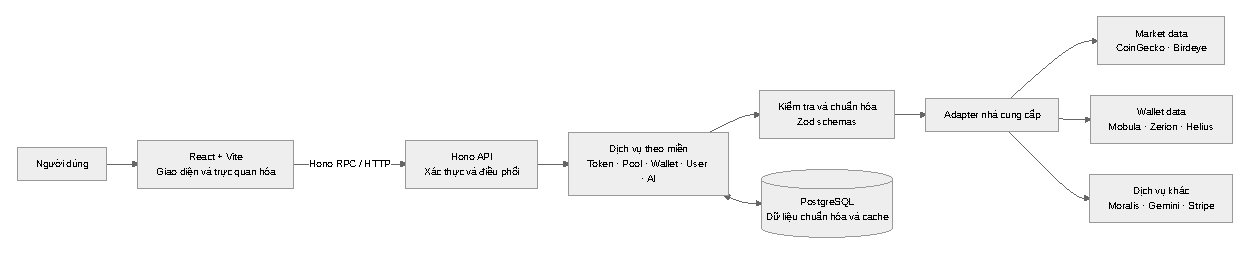
\includegraphics[width=\textwidth]{Chapter4/system-architecture.pdf}
    \caption{Kiến trúc tổng thể của hệ thống Yoca}
    \label{fig:system-architecture}
\end{figure}

Giao diện không gọi trực tiếp API của các nhà cung cấp. Mọi yêu cầu đi qua backend để xác thực, kiểm tra dữ liệu đã lưu, gọi nguồn bên ngoài khi cần và chuyển phản hồi về mô hình nội bộ. Ranh giới này đặc biệt quan trọng vì các provider không chỉ khác tên trường mà còn khác cách biểu diễn token, thời gian, giá trị rỗng và phạm vi lịch sử. Nếu để từng màn hình tự xử lý những khác biệt đó, thay đổi từ một provider sẽ lan sang nhiều thành phần giao diện.

Đây là kiến trúc phân lớp theo trách nhiệm, không phải sự phân tách tuyệt đối. Trong mã nguồn còn tồn tại cả cấu trúc \texttt{routes/services} cũ và một số module mới được gom theo miền. Nhóm chúng em xem đây là kết quả của cách nâng cấp tăng dần: chức năng mới được hoàn thiện và thay thế luồng cũ, sau đó phần không còn được sử dụng mới được loại bỏ. Cách làm này giúp hệ thống tiếp tục hoạt động trong lúc dữ liệu và yêu cầu thay đổi, nhưng cũng tạo ra khoản nợ cần tiếp tục đồng nhất hóa sau đồ án.

\section{Hợp đồng dữ liệu từ giao diện đến nhà cung cấp}

Ứng dụng dùng TypeScript ở cả client và server. Backend xuất kiểu của toàn bộ cây route Hono, còn client khởi tạo RPC client từ chính kiểu đó. Nhờ vậy, đường dẫn, tham số và kiểu phản hồi được kiểm tra ngay trong quá trình phát triển thay vì phải duy trì thêm một bộ khai báo API viết tay. Đây là lý do nhóm chọn Hono: với quy mô hiện tại, Hono RPC tạo được hợp đồng end-to-end mà không cần sinh mã từ một đặc tả trung gian \cite{hono}.

Kiểu TypeScript chỉ tồn tại trong lúc phát triển nên không thể bảo đảm dữ liệu trả về từ Internet là đúng. Trước khi đưa phản hồi của provider vào nghiệp vụ hoặc cơ sở dữ liệu, các service quan trọng sử dụng Zod để kiểm tra cấu trúc ở runtime. Khi một trường sai kiểu, thiếu ngoài dự kiến hoặc mang hình dạng khác tài liệu, hệ thống dừng tại biên tích hợp và trả lỗi thay vì tiếp tục tính toán bằng dữ liệu mơ hồ. Nhóm chúng em chủ ý chọn cách \textit{fail-fast} này vì một kết quả PnL trông hợp lý nhưng được tính từ dữ liệu sai nguy hiểm hơn một yêu cầu thất bại có thể truy vết.

Zod cho phép định nghĩa schema và kiểm tra dữ liệu không đáng tin cậy ngay khi chương trình đang chạy, phù hợp với vai trò bảo vệ biên tích hợp của Yoca \cite{zod}.

Việc kiểm tra chặt cũng làm lộ ra một khó khăn thực tế: tài liệu của provider không phải lúc nào cũng nói rõ trường nào có thể rỗng. Chẳng hạn, địa chỉ token là định danh chắc chắn hơn tên hoặc ký hiệu; các chỉ số biến động giá cũng có thể không tồn tại với token mới hay ít thanh khoản. Lược đồ nội bộ vì vậy không sao chép nguyên xi một phản hồi mẫu, mà chấp nhận giá trị thiếu ở nơi dữ liệu thực tế đòi hỏi và giữ ràng buộc chặt cho các định danh cốt lõi.

Một contract đại diện là API lịch sử cảnh báo. Client gọi \texttt{GET /api/alerts/history} với \texttt{page} và \texttt{limit}; server lấy \texttt{userId} từ phiên xác thực thay vì nhận từ query, nhờ đó người dùng không thể yêu cầu lịch sử của tài khoản khác. Phản hồi gồm danh sách theo thứ tự mới nhất, tổng số bản ghi và số chưa đọc. Mỗi item giữ nguồn cảnh báo, message, severity, trạng thái email/Discord, thời điểm gửi và \texttt{readAt}. Khi cập nhật \texttt{PATCH /api/alerts/history/:id/read}, điều kiện truy vấn đồng thời dùng history ID và user ID; bản ghi không thuộc tài khoản được trả như không tồn tại.

\begin{table}[H]
\centering
\caption{Contract đại diện của API Alert History}
\label{tab:alert-history-contract}
\renewcommand{\arraystretch}{1.15}
\small
\begin{tabularx}{\textwidth}{|p{3.2cm}|X|X|}
\hline
\textbf{Thành phần} & \textbf{Dữ liệu hợp lệ} & \textbf{Hành vi khi không hợp lệ/không đầy đủ} \\
\hline
List history & \texttt{page >= 1}, \texttt{1 <= limit <= 100}; user lấy từ JWT & Query sai trả lỗi validation; lỗi database trả 500; không có dữ liệu trả danh sách rỗng cùng tổng bằng 0 \\
\hline
Read state & UUID history và boolean \texttt{read}; update được scope bởi user & UUID sai trả 400; ID không tồn tại hoặc thuộc user khác trả 404 \\
\hline
Delivery snapshot & Ít nhất một kênh gửi thành công; lưu attempted/succeeded riêng cho email và Discord & Partial delivery vẫn được lưu đúng trạng thái từng kênh; không kênh nào thành công thì không tạo history \\
\hline
Idempotency & Khóa logic từ user, transaction signature, scope và rule/ví & Webhook retry cùng sự kiện không tạo bản ghi thứ hai \\
\hline
\end{tabularx}
\end{table}

\section{Luồng truy xuất, chuẩn hóa và lưu đệm}

Mẫu truy xuất phổ biến trong backend gồm hai lớp hàm. Hàm \texttt{get*} là điểm vào của route: nó tìm dữ liệu trong cơ sở dữ liệu và đánh giá độ mới. Nếu dữ liệu còn hợp lệ, kết quả được trả ngay; nếu thiếu hoặc đã cũ, hàm gọi luồng \texttt{fetch*}. Luồng thứ hai chịu trách nhiệm truy cập provider, kiểm tra phản hồi, cập nhật cơ sở dữ liệu rồi trả về cùng kiểu dữ liệu nội bộ. Không phải mọi service đều tuân theo đúng tên gọi này, nhưng đây là nguyên tắc chủ đạo đối với dữ liệu thị trường và dữ liệu ví.

Nhóm chúng em không áp dụng fallback nhiều provider một cách mặc định. Mỗi provider được chọn theo phần dữ liệu mà họ có thế mạnh và theo hạn mức còn khả dụng. Token metadata là một trong những nơi cần nhiều nguồn bổ sung, trong khi PnL và lịch sử giao dịch ví hiện dựa chủ yếu vào Mobula; lịch sử tổng tài sản ưu tiên Mobula, còn chuỗi số dư theo từng token tiếp tục dùng Zerion. Helius vẫn giữ vai trò đối với giao dịch on-chain và webhook. Sự phân công theo miền làm giảm số nhánh khó kiểm soát, dù đồng nghĩa hệ thống vẫn phụ thuộc đáng kể vào chất lượng của từng nguồn.

Cơ sở dữ liệu vừa lưu dữ liệu nghiệp vụ, vừa là lớp cache bền vững. Thiết kế bảng không chỉ theo mục tiêu chuẩn hóa mà còn cân nhắc số lần gọi API để hoàn thiện một bản ghi. Nếu một hàng yêu cầu hai hoặc ba endpoint khác nhau nhưng các phần dữ liệu có chu kỳ cập nhật khác nhau, việc tách chúng thành các bảng nhỏ giúp chỉ làm mới phần đã cũ. Khi provider trả kèm thông tin hữu ích, service có thể cập nhật thêm bảng liên quan để tận dụng dữ liệu đã trả phí truy vấn, song việc cập nhật chéo phải đi qua khóa và ràng buộc nhất quán.

\section{Thiết kế cơ sở dữ liệu}
\label{sec:thiet_ke_csdl}

\subsection{Mục tiêu và đặc điểm dữ liệu}
\label{subsec:db_muc_tieu}

Cơ sở dữ liệu PostgreSQL của Yoca được thiết kế theo hai lớp có mục đích khác nhau. Lớp thứ nhất là dữ liệu nền tương đối chuẩn hóa, gồm tài khoản, phương thức xác thực, watchlist, nhãn ví, cảnh báo, subscription và thanh toán. Đây là dữ liệu do người dùng hoặc hệ thống sở hữu, cần khóa ngoại và quy tắc xóa rõ ràng. Lớp thứ hai là các read model và cache bền vững cho token, pool, ví, giao dịch và kết quả phân tích. Lớp này ưu tiên khả năng đọc nhanh, tái sử dụng dữ liệu provider và làm mới từng phần hơn là loại bỏ mọi sự lặp dữ liệu.

Dữ liệu trong Yoca có hai đặc điểm. Dữ liệu tài khoản và thanh toán cần quan hệ rõ ràng, ràng buộc khóa ngoại và quy tắc xóa nhất quán. Ngược lại, phần lớn dữ liệu blockchain là dữ liệu công khai được định danh bằng token address, wallet address hoặc transaction signature. Các bảng này thường không phụ thuộc vào một bảng gốc duy nhất mà được liên kết theo khóa nghiệp vụ.

Schema được định nghĩa bằng Drizzle ORM. Kiểu dữ liệu, primary key, unique constraint và foreign key được đặt trong mã TypeScript, giúp truy vấn backend và cấu trúc PostgreSQL dùng chung một định nghĩa. Tuy nhiên, schema vật lý không phải lúc nào cũng trùng với mô hình khái niệm: wallet address, token address và signature thường là khóa nghiệp vụ liên kết nhiều bảng nhưng không bị buộc phải tham chiếu đến một bảng cha.

\subsection{Phân nhóm dữ liệu theo miền nghiệp vụ}
\label{subsec:db_phan_nhom}

Cấu trúc lưu trữ được chia theo các miền identity/payment, token/market, wallet/analysis, transaction, alert và content/AI. Hình~\ref{fig:db_overview} chỉ thể hiện quan hệ khái niệm giữa các miền; các ERD phía sau mới phân biệt foreign key vật lý với liên hệ bằng address hoặc signature.

\begin{figure}[H]
    \centering
    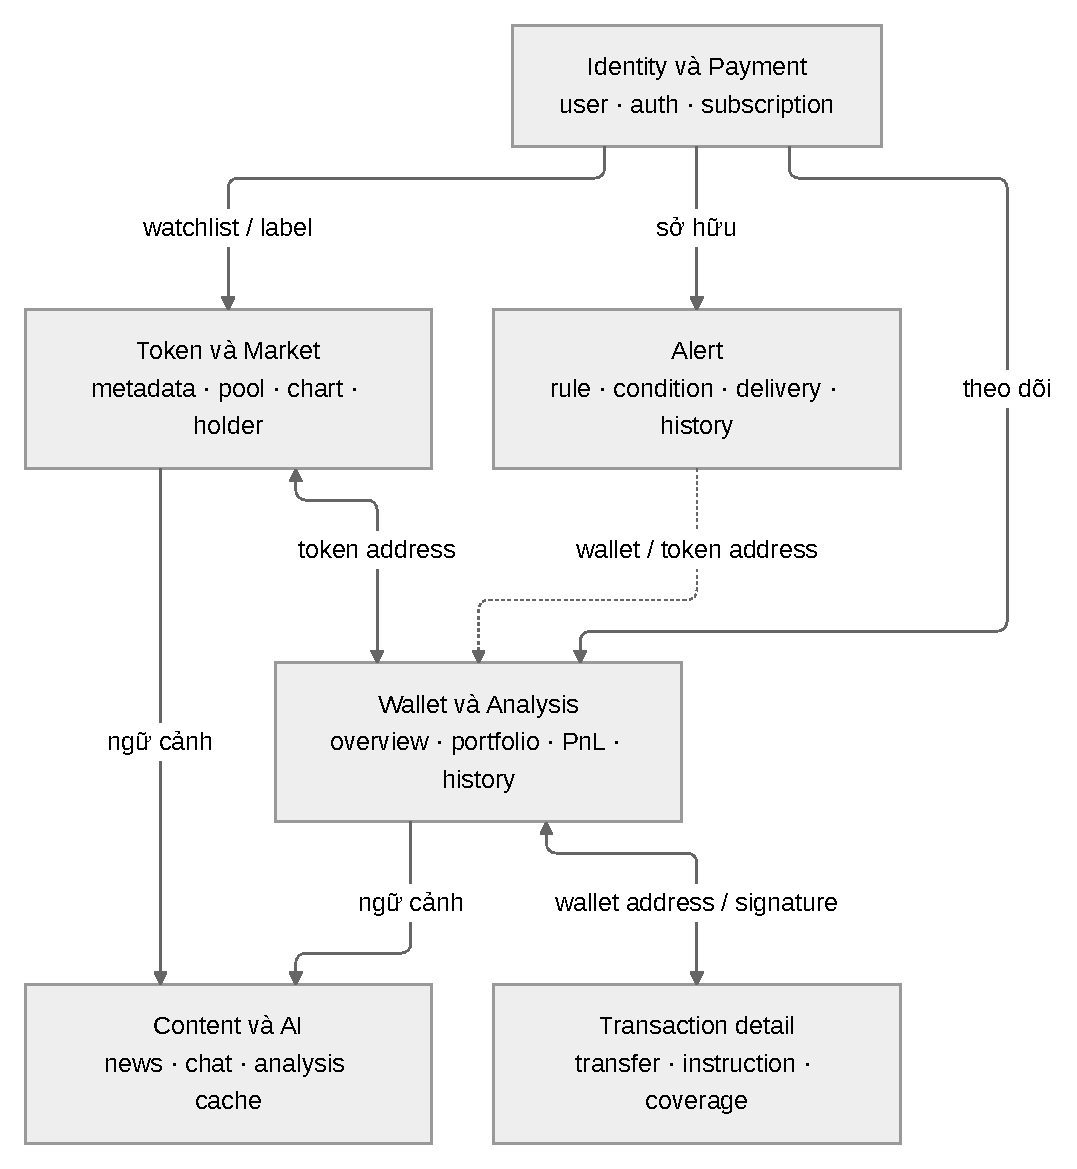
\includegraphics[width=0.9\textwidth,height=0.68\textheight,keepaspectratio]{Chapter3/diagrams/database-overview.pdf}
    \caption{Các miền dữ liệu chính và quan hệ khái niệm}
    \label{fig:db_overview}
\end{figure}

Các nhóm trên phục vụ nhu cầu truy vấn khác nhau. Vì vậy, dữ liệu có thể giao nhau về wallet address, token address hoặc transaction signature nhưng không đồng nghĩa các bảng có thể thay thế trực tiếp cho nhau. Cách phân nhóm cũng giúp ERD tổng thể không biến thành một hình quá dài theo chiều ngang và phải thu nhỏ đến mức không đọc được.

\subsection{Sơ đồ thực thể mối quan hệ}
\label{subsec:db_erd}

Schema có nhiều bảng cache nên một ERD duy nhất sẽ khó đọc trên khổ A4. Phần này chia ERD theo miền nghiệp vụ và chỉ giữ primary key, foreign key cùng các cột chính. Đường liền biểu diễn foreign key được khai báo trong PostgreSQL. Đường nét đứt biểu diễn liên hệ logic thông qua address, mint hoặc signature; các liên hệ này được kiểm soát tại service thay vì bằng foreign key.

\begin{figure}[H]
    \centering
    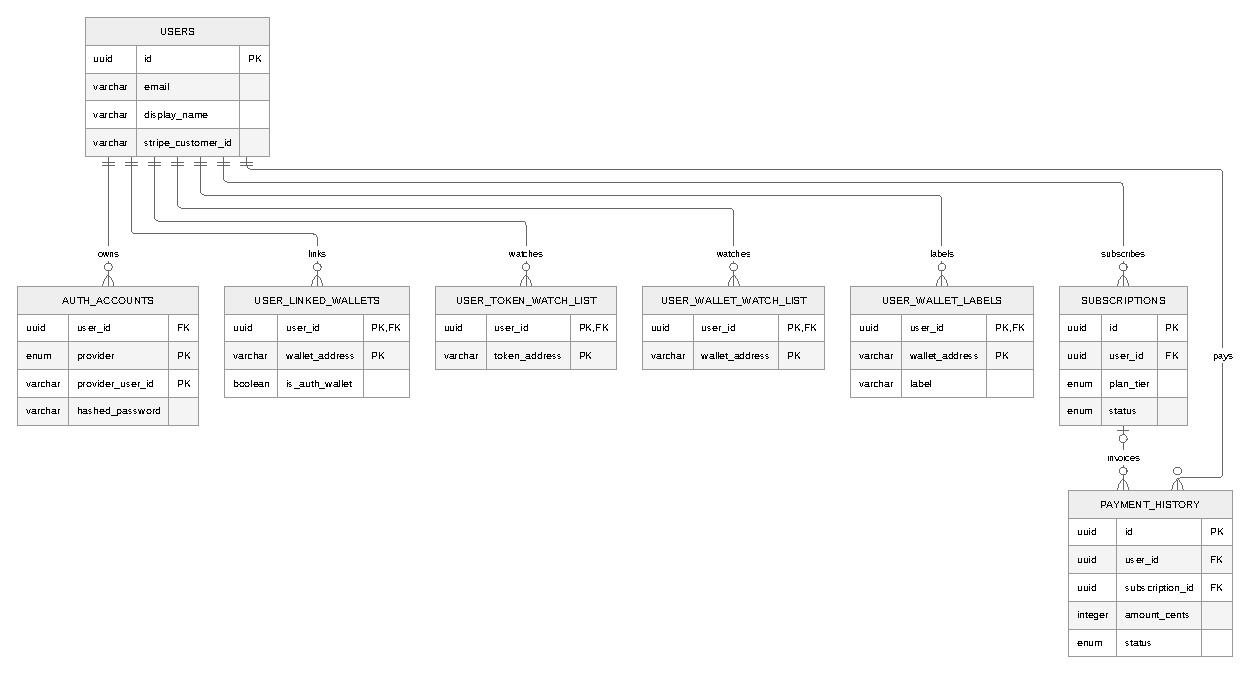
\includegraphics[width=\textwidth,height=0.78\textheight,keepaspectratio]{Chapter3/diagrams/identity-payment.pdf}
    \caption{ERD nhóm tài khoản và thanh toán}
    \label{fig:db_identity_payment}
\end{figure}

Hình~\ref{fig:db_identity_payment} thể hiện dữ liệu có tính sở hữu. Bảng \texttt{users} là gốc của dữ liệu xác thực, cấu hình cá nhân và thanh toán. Các bản ghi phụ thuộc người dùng được xóa theo quan hệ cascade; lịch sử thanh toán giữ được bản ghi khi subscription không còn tồn tại.

\begin{figure}[H]
    \centering
    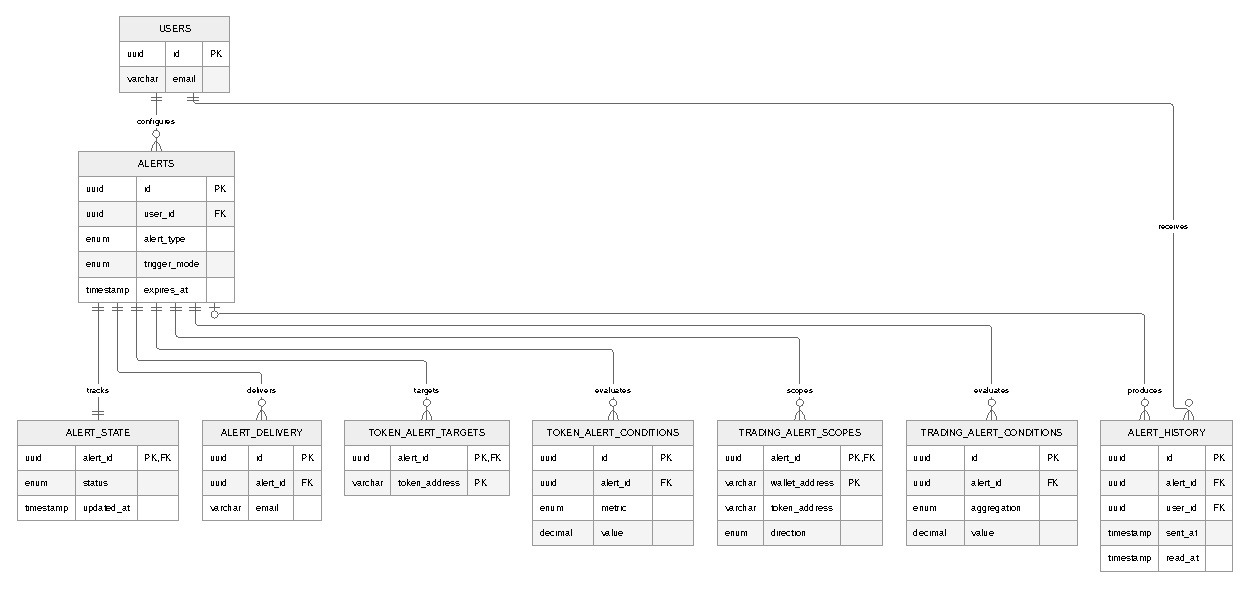
\includegraphics[width=\textwidth,height=0.78\textheight,keepaspectratio]{Chapter3/diagrams/alert-history.pdf}
    \caption{ERD nhóm cảnh báo và lịch sử cảnh báo}
    \label{fig:db_alert_history}
\end{figure}

Hình~\ref{fig:db_alert_history} tách định nghĩa cảnh báo khỏi trạng thái, delivery target và điều kiện kích hoạt. \texttt{alert\_history} lưu sự kiện đã phát sinh để hỗ trợ hiển thị lịch sử và trạng thái đã đọc.

\begin{figure}[H]
    \centering
    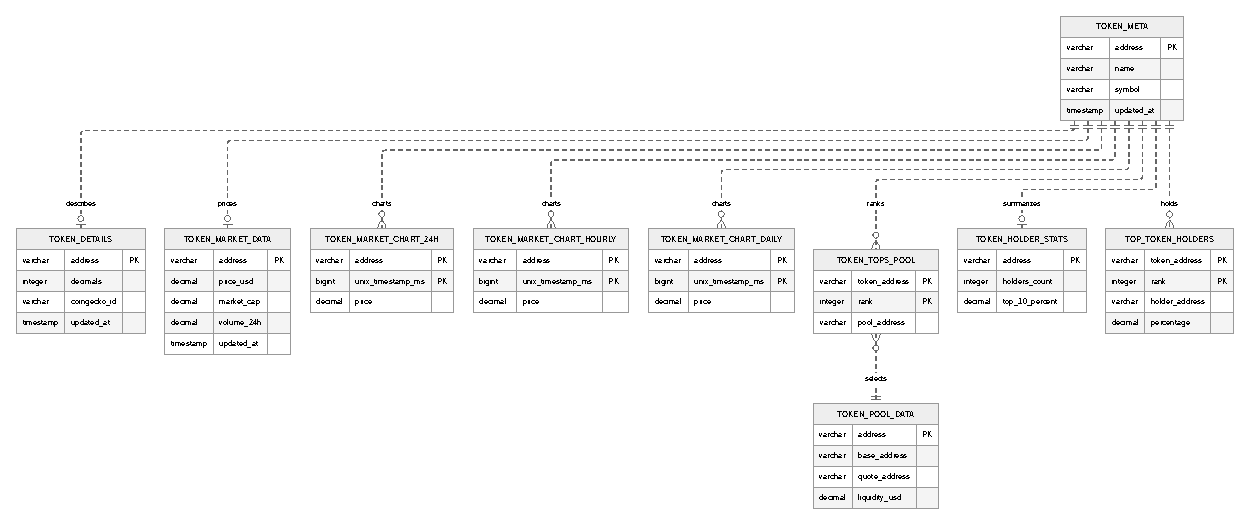
\includegraphics[width=\textwidth,height=0.78\textheight,keepaspectratio]{Chapter3/diagrams/token-market.pdf}
    \caption{ERD nhóm token và dữ liệu thị trường}
    \label{fig:db_token_market}
\end{figure}

Hình~\ref{fig:db_token_market} sử dụng \texttt{token\_meta} như điểm tham chiếu logic. Market snapshot và chart được cập nhật theo address và mốc thời gian. Pool và holder là các read model riêng, chỉ liên kết logic với token.

\begin{figure}[H]
    \centering
    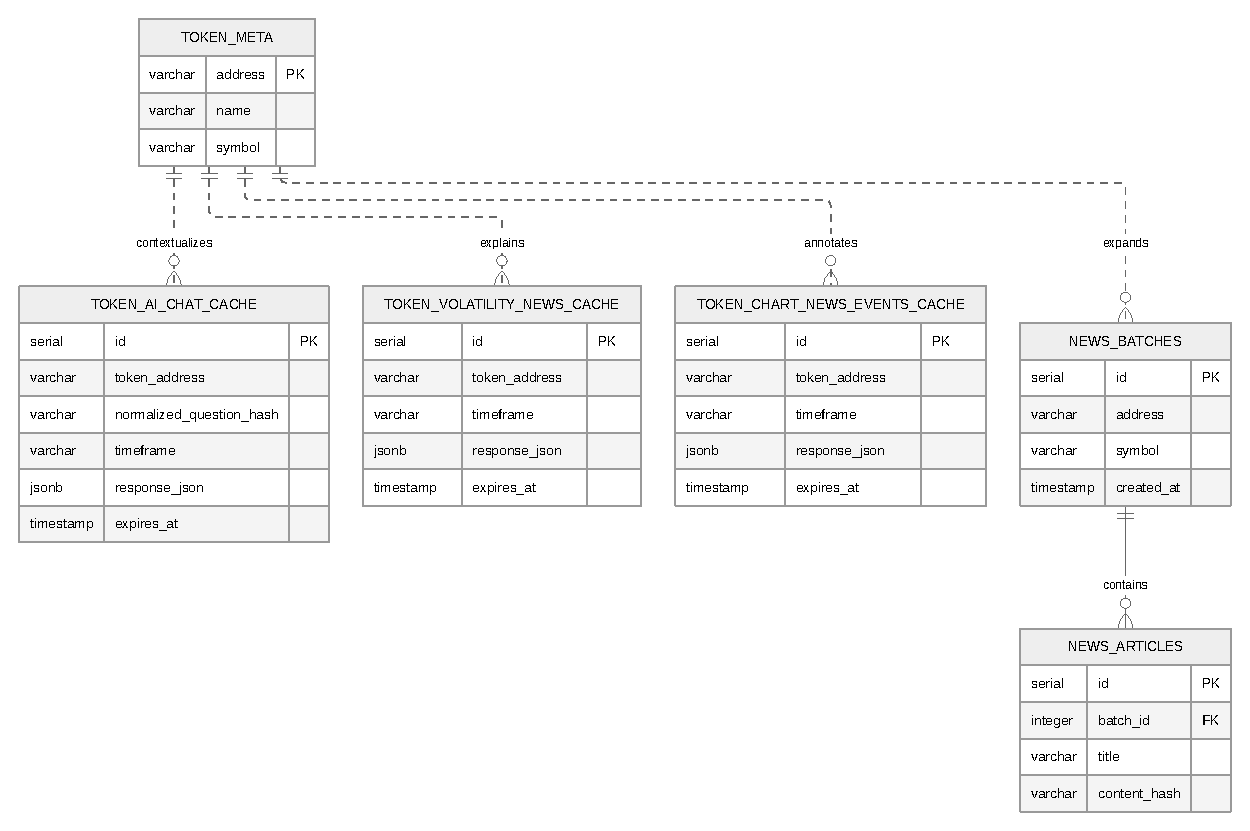
\includegraphics[width=\textwidth,height=0.78\textheight,keepaspectratio]{Chapter3/diagrams/token-content.pdf}
    \caption{ERD nhóm nội dung và AI cache theo token}
    \label{fig:db_token_content}
\end{figure}

Hình~\ref{fig:db_token_content} mô tả các cache phục vụ AI, news event và phần giải thích biến động. News batch có quan hệ khóa ngoại trực tiếp với article; các cache còn lại được ghép với token theo address.

\begin{figure}[H]
    \centering
    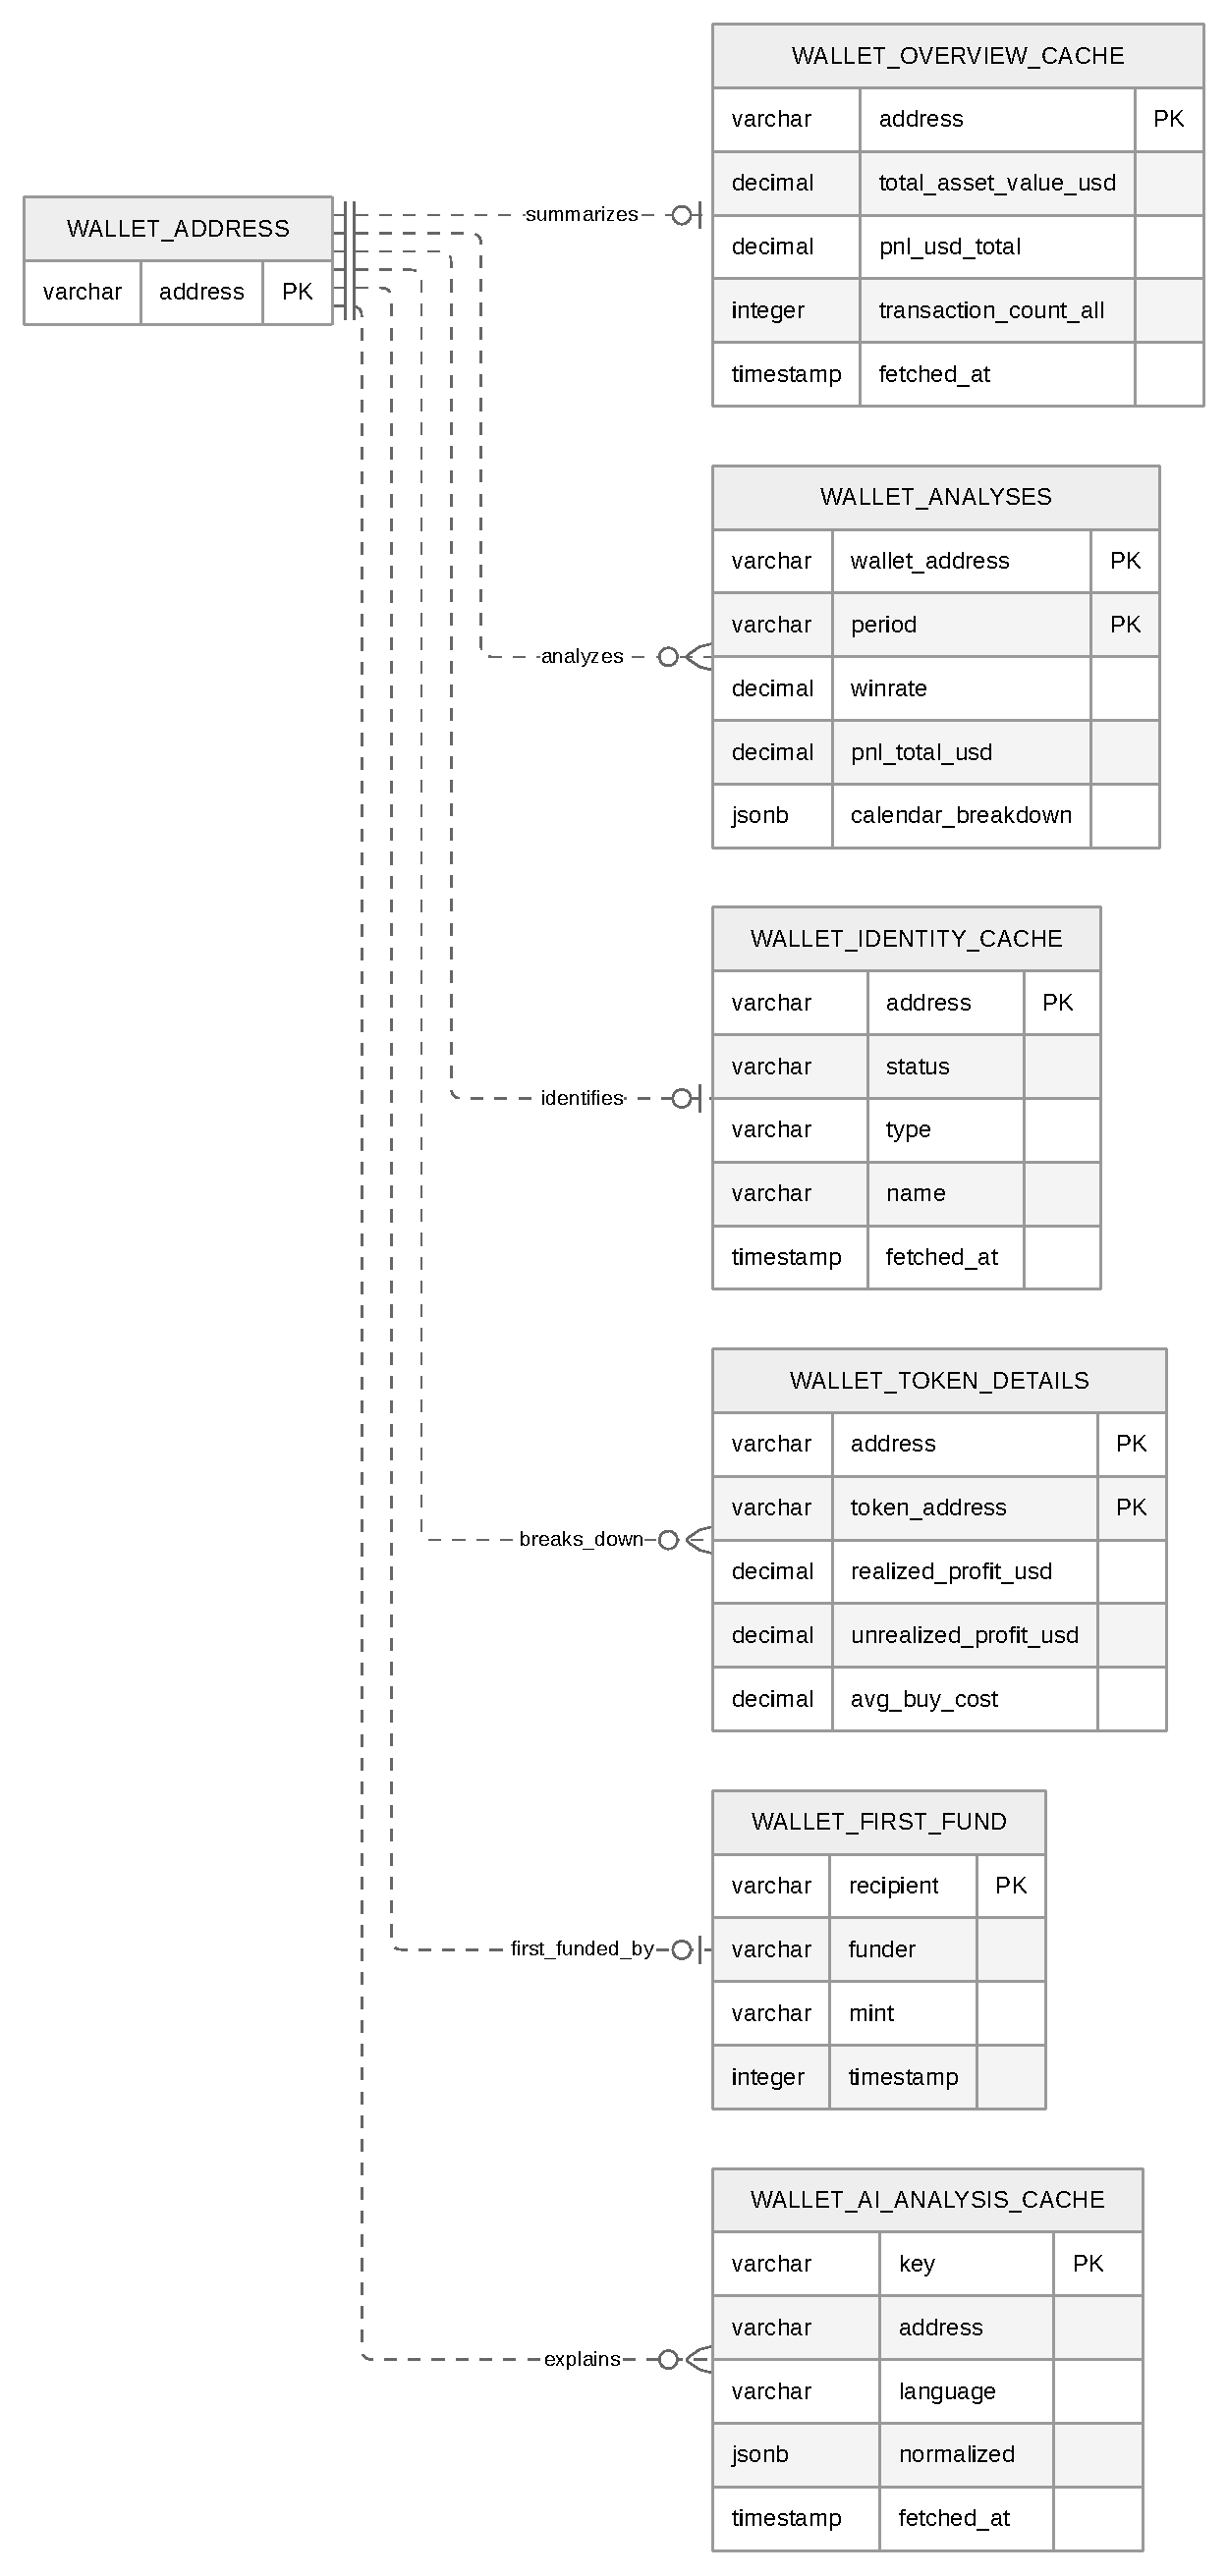
\includegraphics[width=\textwidth,height=0.78\textheight,keepaspectratio]{Chapter3/diagrams/wallet-analytics.pdf}
    \caption{ERD nhóm tổng quan và phân tích ví}
    \label{fig:db_wallet_analytics}
\end{figure}

Hình~\ref{fig:db_wallet_analytics} dùng \texttt{WALLET\_ADDRESS} như một thực thể logic, không phải bảng vật lý. \texttt{wallet\_overview\_cache} cung cấp bản tổng hợp cho trang overview. \texttt{wallet\_analyses} lưu kết quả Mobula theo ví và kỳ phân tích.

\begin{figure}[H]
    \centering
    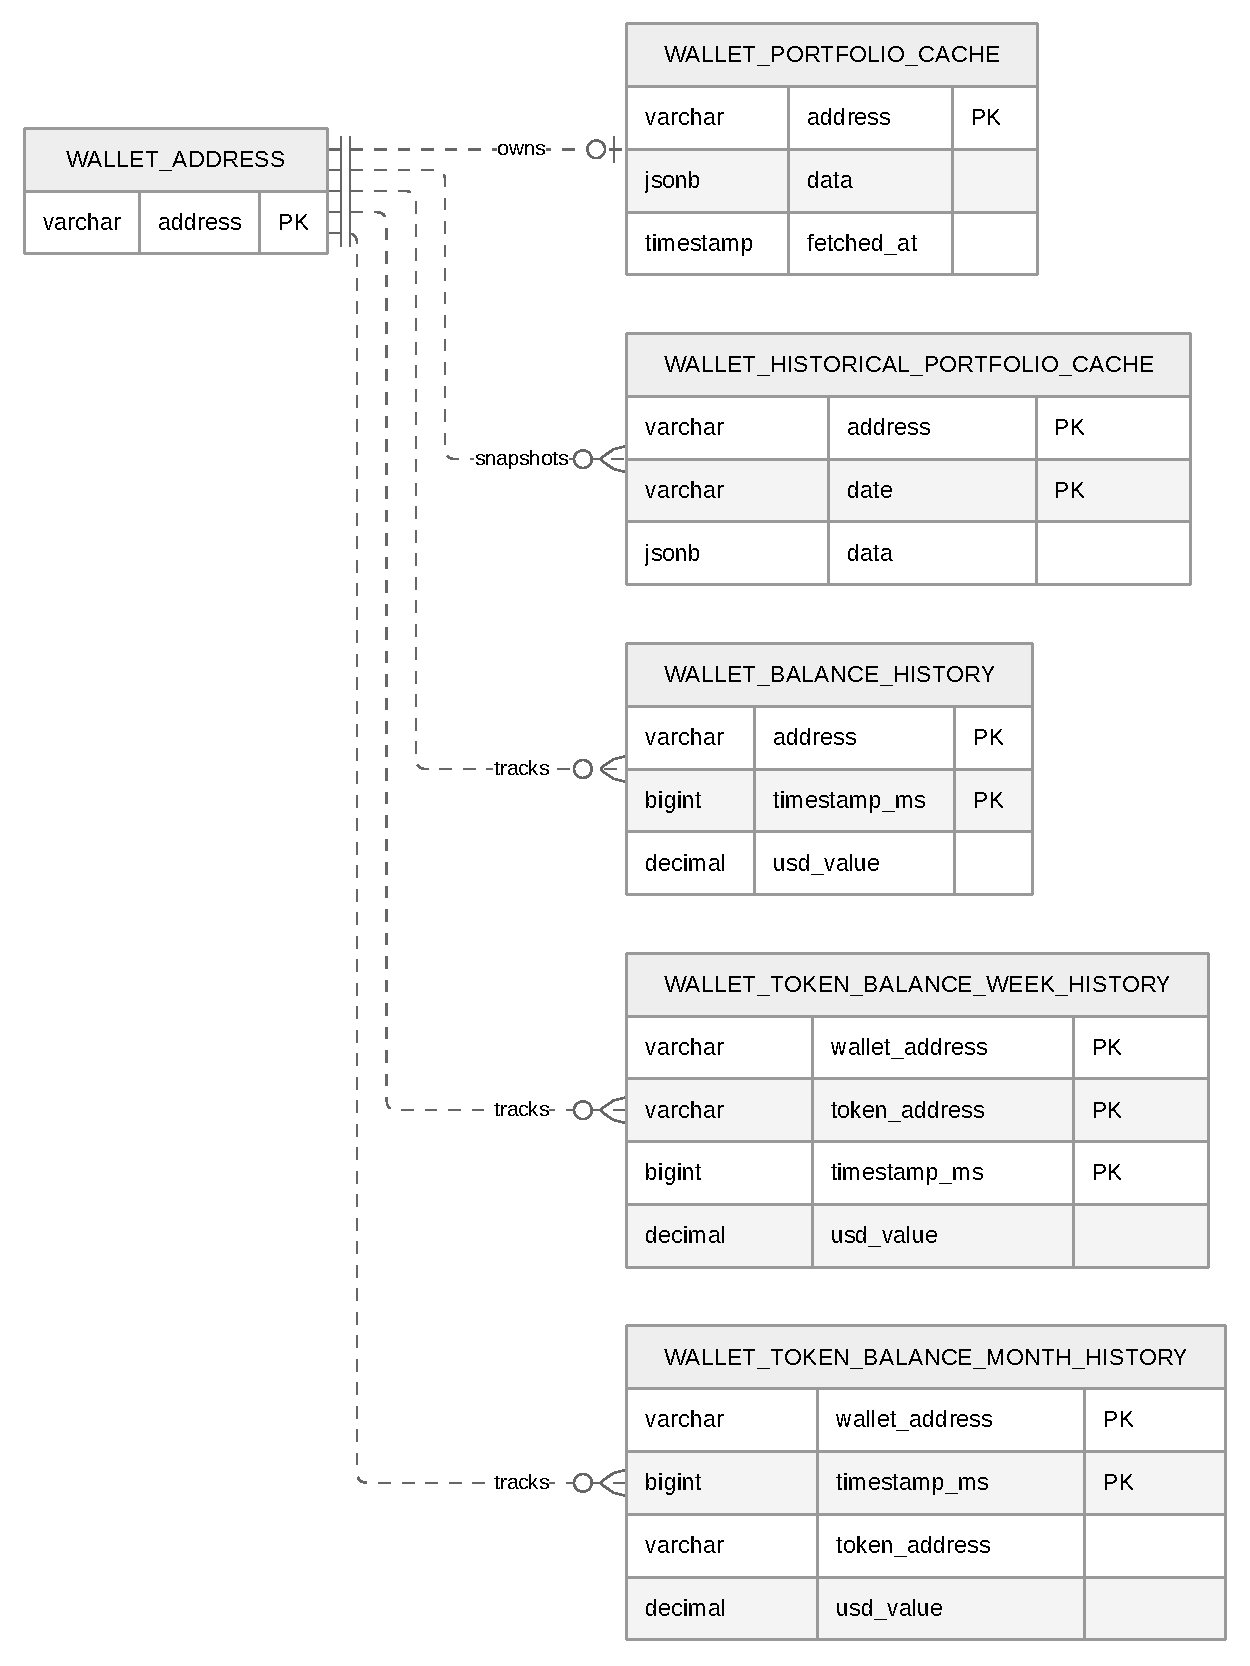
\includegraphics[width=\textwidth,height=0.78\textheight,keepaspectratio]{Chapter3/diagrams/wallet-portfolio-balance.pdf}
    \caption{ERD nhóm portfolio và lịch sử số dư}
    \label{fig:db_wallet_portfolio_balance}
\end{figure}

Hình~\ref{fig:db_wallet_portfolio_balance} phân biệt portfolio hiện tại, snapshot theo ngày, tổng giá trị ví theo thời gian và lịch sử số dư ở cấp token. Các bảng được ghép theo wallet address nhưng không phụ thuộc một bảng wallet vật lý.

\begin{figure}[H]
    \centering
    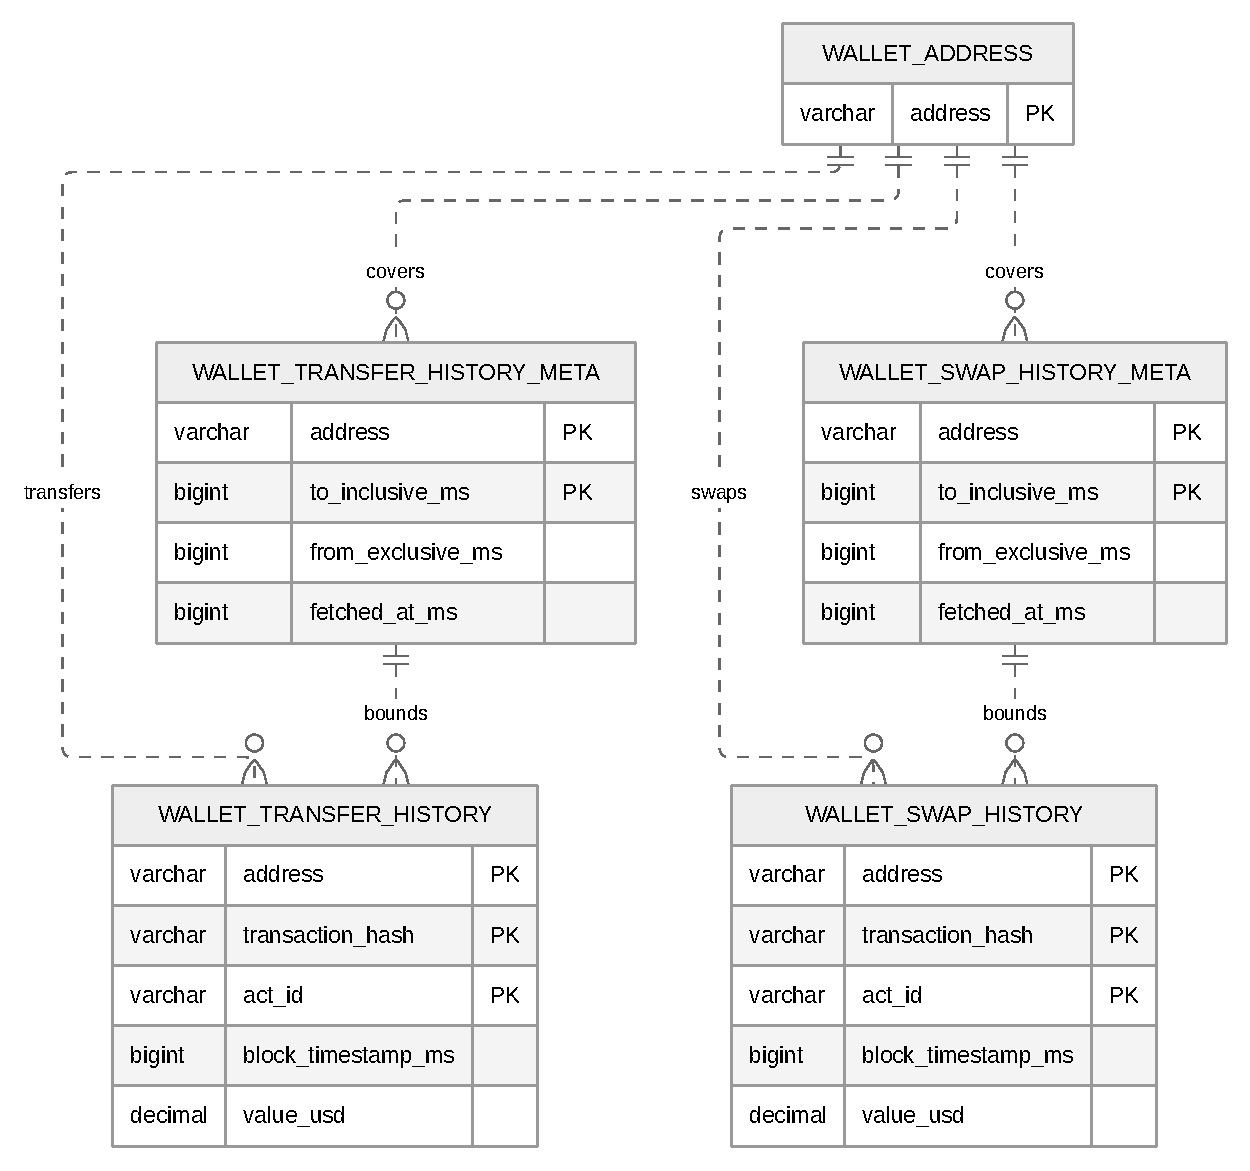
\includegraphics[width=\textwidth,height=0.78\textheight,keepaspectratio]{Chapter3/diagrams/wallet-history.pdf}
    \caption{ERD nhóm lịch sử transfer và swap}
    \label{fig:db_wallet_history}
\end{figure}

Hình~\ref{fig:db_wallet_history} tách dữ liệu lịch sử đã chuẩn hóa khỏi metadata coverage. Các bảng này phục vụ truy vấn phân trang và chỉ tải bổ sung những khoảng thời gian còn thiếu.

\begin{figure}[H]
    \centering
    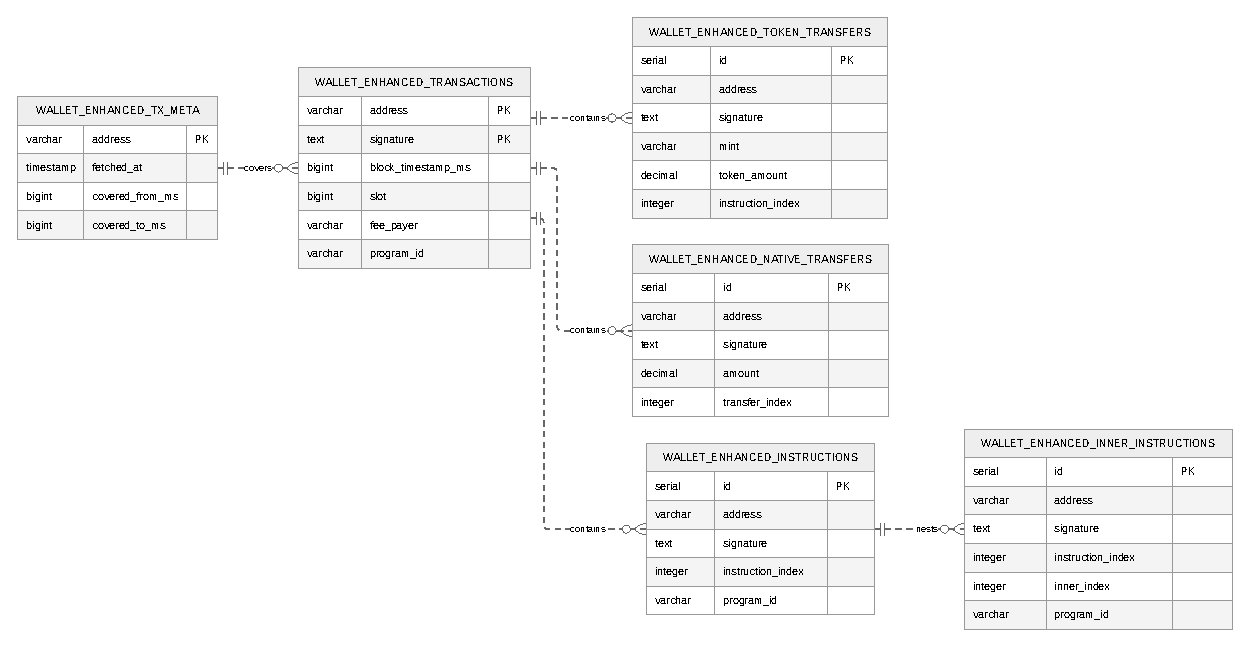
\includegraphics[width=\textwidth,height=0.78\textheight,keepaspectratio]{Chapter3/diagrams/enhanced-transaction-detail.pdf}
    \caption{ERD nhóm chi tiết giao dịch Helius}
    \label{fig:db_enhanced_transaction_detail}
\end{figure}

Hình~\ref{fig:db_enhanced_transaction_detail} mô tả read model chi tiết giao dịch. Bảng transaction cha được ghép với token transfer, native transfer và instruction bằng address cùng signature. Nhóm này phục vụ day activity, transaction detail và wallet analysis; nó không bị thay thế bởi transfer/swap history.

\subsection{Các bảng trọng tâm}
\label{subsec:db_bang_trong_tam}

Bảng~\ref{tab:db_core_tables} tóm tắt các bảng đại diện cho từng miền. Các bảng cache phụ có cùng cách tổ chức không được liệt kê lại để tránh lặp nội dung.

\begin{longtable}{|L{0.27\textwidth}|L{0.25\textwidth}|L{0.38\textwidth}|}
\caption{Các bảng dữ liệu trọng tâm của Yoca}
\label{tab:db_core_tables}\\
\hline
\textbf{Bảng} & \textbf{Khóa chính} & \textbf{Vai trò} \\
\hline
\endfirsthead
\hline
\textbf{Bảng} & \textbf{Khóa chính} & \textbf{Vai trò} \\
\hline
\endhead
\texttt{users} & \texttt{id} & Thông tin tài khoản, cấu hình nhận cảnh báo và Stripe customer. \\
\hline
\texttt{auth\_accounts} & \texttt{provider, provider\_user\_id} & Danh tính đăng nhập bằng password, OAuth hoặc ví Solana. \\
\hline
\texttt{subscriptions} & \texttt{id} & Trạng thái gói dịch vụ và chu kỳ thanh toán. \\
\hline
\texttt{alerts} & \texttt{id} & Định nghĩa cảnh báo, loại cảnh báo, chế độ kích hoạt và thời hạn. \\
\hline
\texttt{alert\_history} & \texttt{id} & Lịch sử cảnh báo đã phát sinh và trạng thái đã đọc. \\
\hline
\texttt{token\_meta} & \texttt{address} & Tên, symbol và hình ảnh cơ bản của token. \\
\hline
\texttt{token\_market\_data} & \texttt{address} & Market snapshot gần nhất, gồm giá, vốn hóa và volume. \\
\hline
\texttt{token\_market\_chart\_*} & \texttt{address, timestamp} & Chuỗi giá 24 giờ, hourly và daily cho biểu đồ. \\
\hline
\texttt{wallet\_overview\_cache} & \texttt{address} & Read model tổng hợp tài sản, volume, PnL và hoạt động của ví. \\
\hline
\texttt{wallet\_analyses} & \texttt{wallet\_address, period} & Kết quả Mobula gồm win rate, PnL, phân phối giao dịch và calendar breakdown. \\
\hline
\texttt{wallet\_transfer\_history} & \texttt{address, transaction\_hash, act\_id} & Lịch sử chuyển token đã chuẩn hóa và hỗ trợ phân trang. \\
\hline
\texttt{wallet\_swap\_history} & \texttt{address, transaction\_hash, act\_id} & Lịch sử swap đã chuẩn hóa theo ví. \\
\hline
\texttt{wallet\_enhanced\_transactions} & \texttt{address, signature} & Transaction cha cho dữ liệu chi tiết từ Helius. \\
\hline
\texttt{chat\_sessions} & \texttt{id} & Phiên chat, context ví và danh sách message. \\
\hline
\texttt{news\_batches} & \texttt{id} & Nhóm bài viết thu thập theo token và thời điểm. \\
\hline
\end{longtable}

\texttt{wallet\_analyses} là read model có kích thước tương đối lớn do lưu cả chỉ số tổng hợp và hai cấu trúc JSONB là \texttt{period\_timeframes} và \texttt{calendar\_breakdown}. Mỗi ví chỉ có một bản ghi cho mỗi kỳ phân tích, nhờ đó dữ liệu Mobula có thể được dùng lại trong thời gian TTL mà không cần gọi provider cho mọi request.

Các bảng \texttt{wallet\_enhanced\_*} lưu chi tiết giao dịch ở mức thấp hơn transfer/swap history. Instruction, inner instruction, fee payer, program ID và native transfer cần thiết cho transaction detail và phân tích hành vi, trong khi history tables ưu tiên danh sách đã chuẩn hóa và phân trang.

\subsection{Cache và quản lý độ mới}
\label{subsec:db_cache}

Cache được kiểm soát bằng ba cơ chế. Cơ chế thứ nhất là TTL dựa trên thời điểm cập nhật. Dữ liệu overview, market hoặc kết quả phân tích được trả trực tiếp khi vẫn còn mới; khi hết TTL, service gọi provider và cập nhật lại bản ghi.

Cơ chế thứ hai là coverage metadata. Với lịch sử ví và enhanced transaction, metadata lưu khoảng thời gian đã đồng bộ. Service so sánh khoảng yêu cầu với khoảng đã có, chỉ tải phần còn thiếu rồi hợp nhất coverage. Cách này tránh tải lại toàn bộ lịch sử của ví.

Cơ chế thứ ba là upsert. Market snapshot, chart point và các cache theo khóa nghiệp vụ sử dụng insert kết hợp conflict handling. Bản ghi mới được thêm khi khóa chưa tồn tại; dữ liệu cũ được cập nhật khi cùng address, timestamp hoặc signature.

\subsection{Toàn vẹn và bảo mật dữ liệu}
\label{subsec:db_toan_ven}

Primary key tổng hợp được dùng cho dữ liệu chuỗi thời gian và lịch sử, ví dụ address kết hợp timestamp hoặc transaction hash. Unique constraint ngăn một transaction detail hoặc chart point bị ghi nhiều lần. Foreign key với quy tắc cascade áp dụng cho dữ liệu thuộc người dùng như auth account, watchlist, alert và subscription.

Không phải mọi liên hệ logic đều được chuyển thành foreign key. Wallet address và token address đến từ blockchain, có thể xuất hiện trước khi metadata tương ứng được tải. Việc bắt buộc foreign key trong trường hợp này sẽ làm gián đoạn luồng đồng bộ. Service chịu trách nhiệm chuẩn hóa address và giữ quy tắc ghép dữ liệu nhất quán.

Dữ liệu công khai từ blockchain được tách khỏi dữ liệu cá nhân. Các truy vấn profile, watchlist, cảnh báo, chat và thanh toán phải được giới hạn theo user ID đã xác thực. Password chỉ được lưu dưới dạng hash; API key và secret của provider không được lưu trong các bảng nghiệp vụ.

% TODO(runtime): Hoàn thiện ghi alert_history sau khi delivery thành công.
% TODO(runtime): Bổ sung API lấy lịch sử, đánh dấu đã đọc và chống gửi trùng.

\subsection{Tổng kết thiết kế cơ sở dữ liệu}
\label{subsec:db_tong_ket}

Thiết kế cơ sở dữ liệu kết hợp dữ liệu quan hệ với các read model cache theo miền nghiệp vụ. Các bảng user, payment và alert ưu tiên ràng buộc quan hệ. Các bảng token và wallet ưu tiên khả năng đồng bộ, truy vấn theo address và tái sử dụng dữ liệu provider. Việc tách overview, history, analysis và transaction detail giúp mỗi endpoint đọc đúng cấu trúc cần thiết thay vì phụ thuộc vào một bảng giao dịch chung.



\section{Lựa chọn công nghệ và giới hạn của thiết kế}

React được chọn vì mô hình thành phần phù hợp với giao diện có nhiều bảng, biểu đồ và trạng thái tương tác dùng lại; Vite cung cấp máy chủ phát triển và cơ chế cập nhật mô-đun nhanh \cite{react,vite}. ECharts đảm nhiệm phần lớn biểu đồ tài chính \cite{echarts}, trong khi các cấu trúc quan hệ giao dịch cần một thành phần đồ thị tương tác riêng. Ở backend, Drizzle được chọn vì cách khai báo lược đồ gần với SQL và cho phép nhóm kiểm soát trực tiếp truy vấn, điều quan trọng khi cache và dữ liệu lịch sử cần các thao tác upsert hoặc truy vấn theo khoảng \cite{drizzle}.

Những lựa chọn trên ưu tiên tốc độ phát triển và khả năng nhìn thấy lỗi sớm, nhưng không tự động tạo ra một hệ thống hoàn toàn nhất quán. Hono RPC chỉ bảo vệ hợp đồng giữa client và server; Zod bảo vệ dữ liệu ở runtime; ràng buộc cơ sở dữ liệu bảo vệ trạng thái đã lưu; còn kiểm thử vẫn cần thiết để xác nhận hành vi kết hợp giữa các lớp. Việc phân biệt các lớp bảo vệ này giúp nhóm không xem ``strongly typed'' như một sự thay thế cho kiểm thử.

Ở phía giao diện, Carbon Design System từng được chọn làm nền tảng chung, nhưng việc hiện thực không được duy trì đồng đều trong suốt quá trình phát triển. Một số màn hình mới kết hợp thành phần tự xây dựng, SCSS và utility class, trong khi một số bảng cũ vẫn giữ cấu trúc Carbon. Nhóm chúng em chấp nhận trình bày đây là hạn chế về tính nhất quán và khả năng bảo trì, thay vì mô tả giao diện như một design system đã hoàn thiện. Trong đợt hoàn thiện cuối, nhóm ưu tiên đồng nhất các luồng chính; những bảng cũ chưa chuyển đổi hoàn toàn được ghi nhận rõ như một giới hạn của phiên bản hiện tại.

Localization được tổ chức thành một lớp dùng chung độc lập với từng trang. Locale tiếng Anh đóng vai trò cấu trúc gốc; locale tiếng Việt phải giữ cùng hệ thống key và biến nội suy. Kiểu TypeScript được dùng để phát hiện key thiếu, key sai và biến interpolation không tương thích trong lúc phát triển. Hook \texttt{useLocalization} cung cấp đồng thời hàm dịch và formatter cho số, phần trăm, token unit, ngày giờ và tiền tệ. Các formatter nhận giá trị tài chính gốc bằng USD; với locale Việt Nam, lớp hiển thị áp dụng tỷ giá USD--VND rồi định dạng theo quy ước VND. Cách tách này giữ phép tính và API ở một đơn vị thống nhất, đồng thời tránh mỗi component tự quy đổi theo một công thức khác nhau.

\section{Kết chương}

Chương 4 đã xác định Yoca là một monolith phân lớp theo miền, có hợp đồng kiểu xuyên suốt giữa client và server, biên kiểm tra runtime cho dữ liệu bên ngoài, cùng cơ chế lưu trữ ưu tiên tái sử dụng dữ liệu đã đồng bộ. Kiến trúc này phản ánh sự cân bằng giữa lược đồ chuẩn hóa, hạn mức API và khả năng phát triển của nhóm. Trên nền thiết kế đó, Chương 5 trình bày kết quả triển khai, những khó khăn đã gặp và mức độ đáp ứng của hệ thống.


\chapter{Triển khai thực nghiệm và Đánh giá}
\label{Chapter4}
Chương này trình bày quá trình triển khai thực nghiệm hệ thống Yoca dựa trên kiến trúc và các luồng nghiệp vụ đã được thiết kế ở Chương 3, bao gồm môi trường triển khai, kết quả hiện thực các chức năng cốt lõi, những thách thức kỹ thuật và giải pháp được áp dụng. Đồng thời, chương trình bày kết quả kiểm thử và đánh giá hệ thống về khả năng vận hành, hiệu năng, độ ổn định và mức độ đáp ứng các yêu cầu đã đặt ra.

\section{Môi trường và công cụ triển khai}
\label{sec:moi_truong_trien_khai}
% Cấu hình các biến môi trường (ENV), quản lý API Key (CoinGecko, Helius, Moralis).

\subsection{Tổ chức môi trường triển khai}

Yoca được triển khai theo mô hình ứng dụng web full-stack, gồm phần giao diện và máy chủ API được tổ chức trong cùng một monorepo. Hai thành phần cùng sử dụng TypeScript và chia sẻ các kiểu dữ liệu cần thiết, qua đó duy trì sự thống nhất trong quá trình trao đổi dữ liệu và phát triển chức năng.

Phần giao diện được xây dựng bằng React 19 và Vite 7, đảm nhiệm việc trình bày dữ liệu và xử lý tương tác của người dùng. Phần máy chủ vận hành trên Node.js với Hono, chịu trách nhiệm xác thực, xử lý nghiệp vụ, chuẩn hóa dữ liệu và kết nối với các dịch vụ bên ngoài. PostgreSQL được sử dụng làm cơ sở dữ liệu chính, kết hợp với Drizzle ORM để quản lý lược đồ và truy vấn dữ liệu. Redis được sử dụng cho các trường hợp cần lưu trữ đệm và tái sử dụng kết quả truy vấn.

Các thành phần trực quan hóa được xây dựng chủ yếu bằng ECharts; riêng dữ liệu có cấu trúc mạng lưới như luồng giao dịch và quan hệ giữa các ví được biểu diễn dưới dạng đồ thị tương tác. Hệ thống cũng hỗ trợ kết xuất dữ liệu và kết quả phân tích thành PDF, bảng tính và hình ảnh để phục vụ việc lưu trữ, đối chiếu và lập báo cáo.

\subsection{Tích hợp nguồn dữ liệu}
\label{subsec:tich_hop_nguon_du_lieu}
Yoca tổng hợp dữ liệu từ nhiều nhà cung cấp chuyên biệt theo từng miền nghiệp vụ, thay vì phụ thuộc vào một nguồn duy nhất.
\begin{itemize}
    \item Dữ liệu thị trường và token: CoinGecko và GeckoTerminal cung cấp giá, vốn hóa, khối lượng, lịch sử giá và thông tin tokenomics. Birdeye bổ sung dữ liệu portfolio, snapshot lịch sử danh mục ví và dữ liệu holder. Moralis và Mobula cung cấp dữ liệu pool, nhà đầu tư và phân phối holder theo phân lớp.
    \item Dữ liệu on-chain: Helius Enhanced API và Solana RPC được sử dụng để truy xuất lịch sử giao dịch, theo dõi webhook và xác minh giao dịch on-chain. Helius cung cấp dạng giao dịch đã được phân tích sẵn (enhanced transactions), giúp giảm đáng kể khối lượng phân tích thủ công.
    \item Tin tức và nội dung: Tin tức liên quan đến token được tổng hợp từ nhiều luồng RSS và kết quả tìm kiếm web, sau đó được chuẩn hóa và loại trùng theo địa chỉ URL trước khi lưu trữ.
    \item AI và thanh toán: Gemini (Google GenAI) được tích hợp trong các chức năng giải thích dữ liệu bằng ngôn ngữ tự nhiên, bao gồm tóm tắt hành vi ví, diễn giải wash trading và hỗ trợ hội thoại. Stripe xử lý thanh toán thẻ, trong khi giao dịch thanh toán bằng Solana được xác minh độc lập phía máy chủ thông qua Helius RPC trước khi ghi nhận quyền sử dụng.
\end{itemize}

Cấu hình hệ thống được tách thành hai nhóm rõ ràng. Các giá trị công khai như địa chỉ máy chủ API, khóa công khai Stripe và cấu hình mạng Solana được cung cấp cho giao diện thông qua biến môi trường Vite (tiền tố \texttt{VITE\_}). Các giá trị nhạy cảm như khóa API nhà cung cấp, chuỗi kết nối cơ sở dữ liệu, khóa ký phiên đăng nhập và khóa bí mật Stripe chỉ được nạp ở phía máy chủ và không bao giờ được gửi về giao diện.

\section{Quy trình tích hợp và triển khai hệ thống}
\label{sec:quy_trinh_trien_khai}

\subsection{Quản lý mã nguồn và môi trường}
Mã nguồn client và server được quản lý trong cùng một Git repository dưới dạng npm workspace. Cấu trúc này cho phép nhóm phát triển hai phần độc lập nhưng vẫn dùng chung phiên bản TypeScript và hợp đồng kiểu Hono. Các thay đổi về route hoặc schema thường cần được đối chiếu với consumer tương ứng trước khi tích hợp, đặc biệt ở các miền Wallet và Payment có nhiều phụ thuộc.

Cấu hình runtime được truyền qua biến môi trường. Client chỉ nhận các giá trị có tiền tố \texttt{VITE\_} và được phép xuất hiện trong browser; khóa provider, chuỗi kết nối PostgreSQL, JWT secret và Stripe secret chỉ thuộc server. Repository cung cấp script riêng cho dev, test, lint, build và đồng bộ schema Drizzle. Trong phạm vi báo cáo, nhóm không đưa nội dung tệp \texttt{.env} hoặc giá trị secret vào phụ lục hay ảnh minh họa.

\subsection{Tích hợp liên tục bằng GitHub Actions}

Workflow CI được đặt tại \texttt{.github/workflows/ci.yml} và chạy khi có thay đổi được đẩy lên nhánh \texttt{main}, \texttt{dev} hoặc khi pull request hướng vào \texttt{main}. Pipeline gồm sáu job kiểm tra độc lập: typecheck, lint, test server, test client, build server và build client. Mỗi job checkout cùng revision, cài dependency theo npm workspace rồi thực hiện script tương ứng. Cách tách này giúp nhóm nhìn rõ lỗi thuộc hợp đồng kiểu, quy tắc mã nguồn, regression test hay production build, thay vì gộp mọi bước vào một lệnh khó chẩn đoán.

Các job test chạy Vitest trong từng workspace; build client tạo static artifact bằng Vite, còn build server biên dịch TypeScript và xử lý path alias trước khi Node khởi động. Concurrency được cấu hình theo Git reference để một lần chạy mới có thể hủy lần chạy cũ trên cùng nhánh. Secret provider và deploy hook không được ghi trực tiếp vào workflow; chúng được quản lý bằng GitHub Actions Secrets và biến môi trường của nền tảng triển khai.

Một job thứ bảy, \texttt{deploy}, phụ thuộc vào cả sáu job trên (\texttt{needs}) và chỉ chạy khi sự kiện là \texttt{push} trên nhánh \texttt{main}. Job này gọi hai \texttt{curl POST} tới deploy hook của Render (một cho Static Site, một cho Web Service) được lưu trong GitHub Actions Secrets, tức bước liên kết CI với Render đã được hiện thực chứ không còn là kiến trúc dự kiến.

\subsection{Triển khai và kiểm tra sau triển khai}

Mã nguồn vẫn được giữ trong một monorepo nhưng được triển khai thành hai đơn vị độc lập trên Render. Client là một Static Site: Render checkout source, chạy \texttt{npm install} và \texttt{npm run client:build}, sau đó phân phối thư mục \texttt{client/build} do Vite tạo ra. Vì vậy production không sử dụng Vite development server. Server là một Web Service: Render chạy \texttt{npm run server:build} rồi khởi động \texttt{node server/build/main.js}. Cách tổ chức này giữ lợi ích chia sẻ kiểu của monorepo nhưng cho phép client và server có vòng đời build, biến môi trường và khả năng triển khai riêng.

\begin{figure}[H]
    \centering
    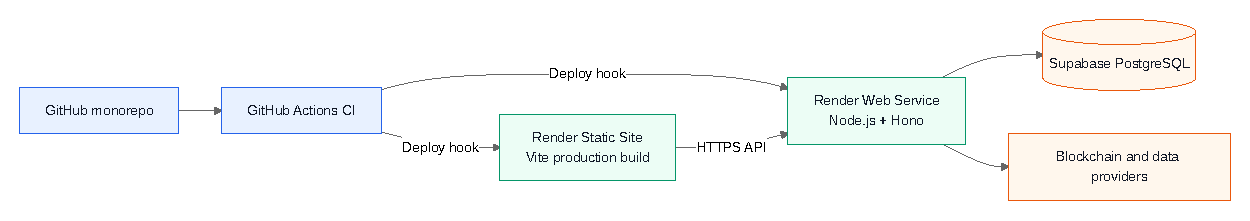
\includegraphics[width=0.9\textwidth]{Chapter4/deployment-architecture.pdf}
    \caption{Kiến trúc tích hợp và triển khai của Yoca}
    \label{fig:deployment-architecture}
\end{figure}

Sau khi các cổng CI đạt, hai deploy hook bí mật được dùng để yêu cầu Render build revision mới cho Static Site và Web Service. Client chỉ nhận các biến \texttt{VITE\_} công khai tại build time; API key, JWT/Stripe secret và chuỗi kết nối database chỉ được cấu hình cho Web Service. PostgreSQL được lưu trên Supabase Free; trong môi trường demo có thể tạo lại, schema Drizzle được đồng bộ bằng quy trình \texttt{db:reset} thay vì duy trì dữ liệu cũ qua migration. Thao tác này không được dùng trên database cần bảo toàn dữ liệu.

Sau triển khai, nhóm kiểm tra endpoint \texttt{/api}, CORS giữa hai domain, SPA rewrite của Static Site và hành trình Market Overview -- Token Pool -- Token Overview -- Wallet -- User -- AI. Free tier có thể tạo cold start hoặc giới hạn tài nguyên, nên báo cáo không xem thời gian phản hồi của lần gọi đầu tiên là một SLA ổn định và không tuyên bố có rollback hay monitoring tự động ngoài phạm vi Render cung cấp sẵn.

\begin{figure}[H]
    \centering
    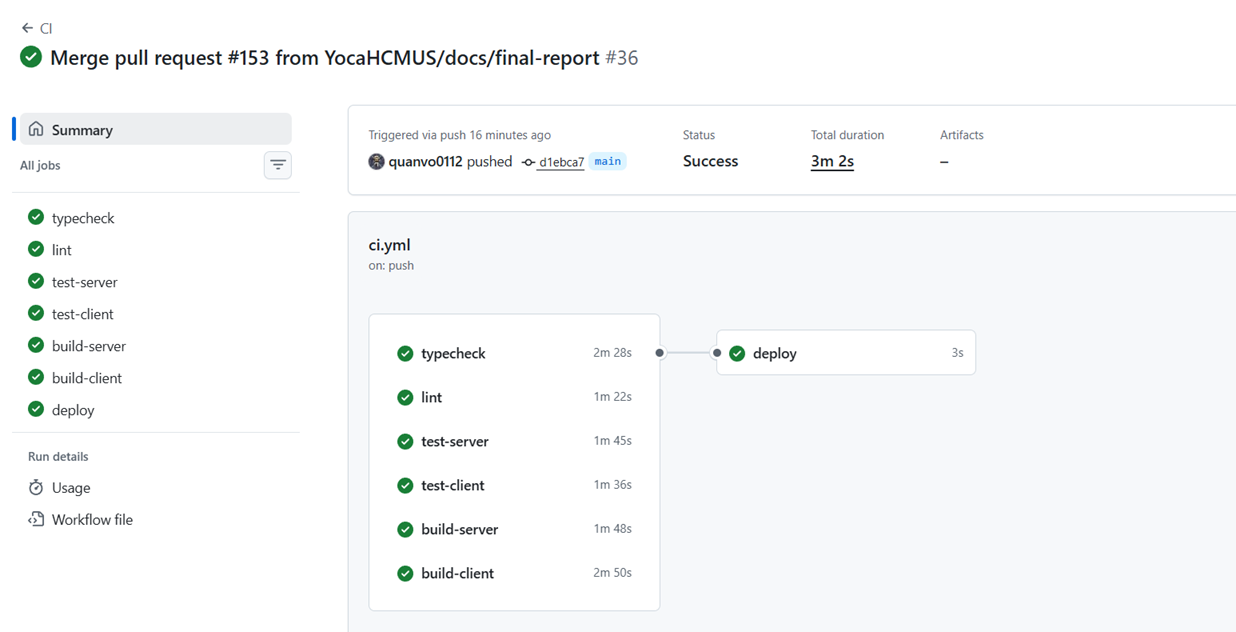
\includegraphics[width=0.95\textwidth]{images/chapter5/github-actions-ci.png}
    \caption{Một lần chạy GitHub Actions thành công trên \texttt{main}: bảy job typecheck, lint, test server/client, build server/client và \texttt{deploy} đều đạt, tổng thời gian 3m2s}
    \label{fig:github-actions-ci}
\end{figure}

Job \texttt{deploy} gọi hai deploy hook của Render; Hình~\ref{fig:render-deployment-frontend} và Hình~\ref{fig:render-deployment-backend} xác nhận cả hai service đã build xong và đang ở trạng thái Live. Yoca hiện chạy thật trên tên miền \texttt{yoca.id.vn}: Static Site \texttt{yoca-frontend} phục vụ giao diện tại địa chỉ này, Web Service \texttt{yoca-backend} phục vụ API tại \texttt{yoca-backend.onrender.com} và đã ghi nhận các request \texttt{GET /api} trả về 200 trong log thời gian thực.

\begin{figure}[H]
    \centering
    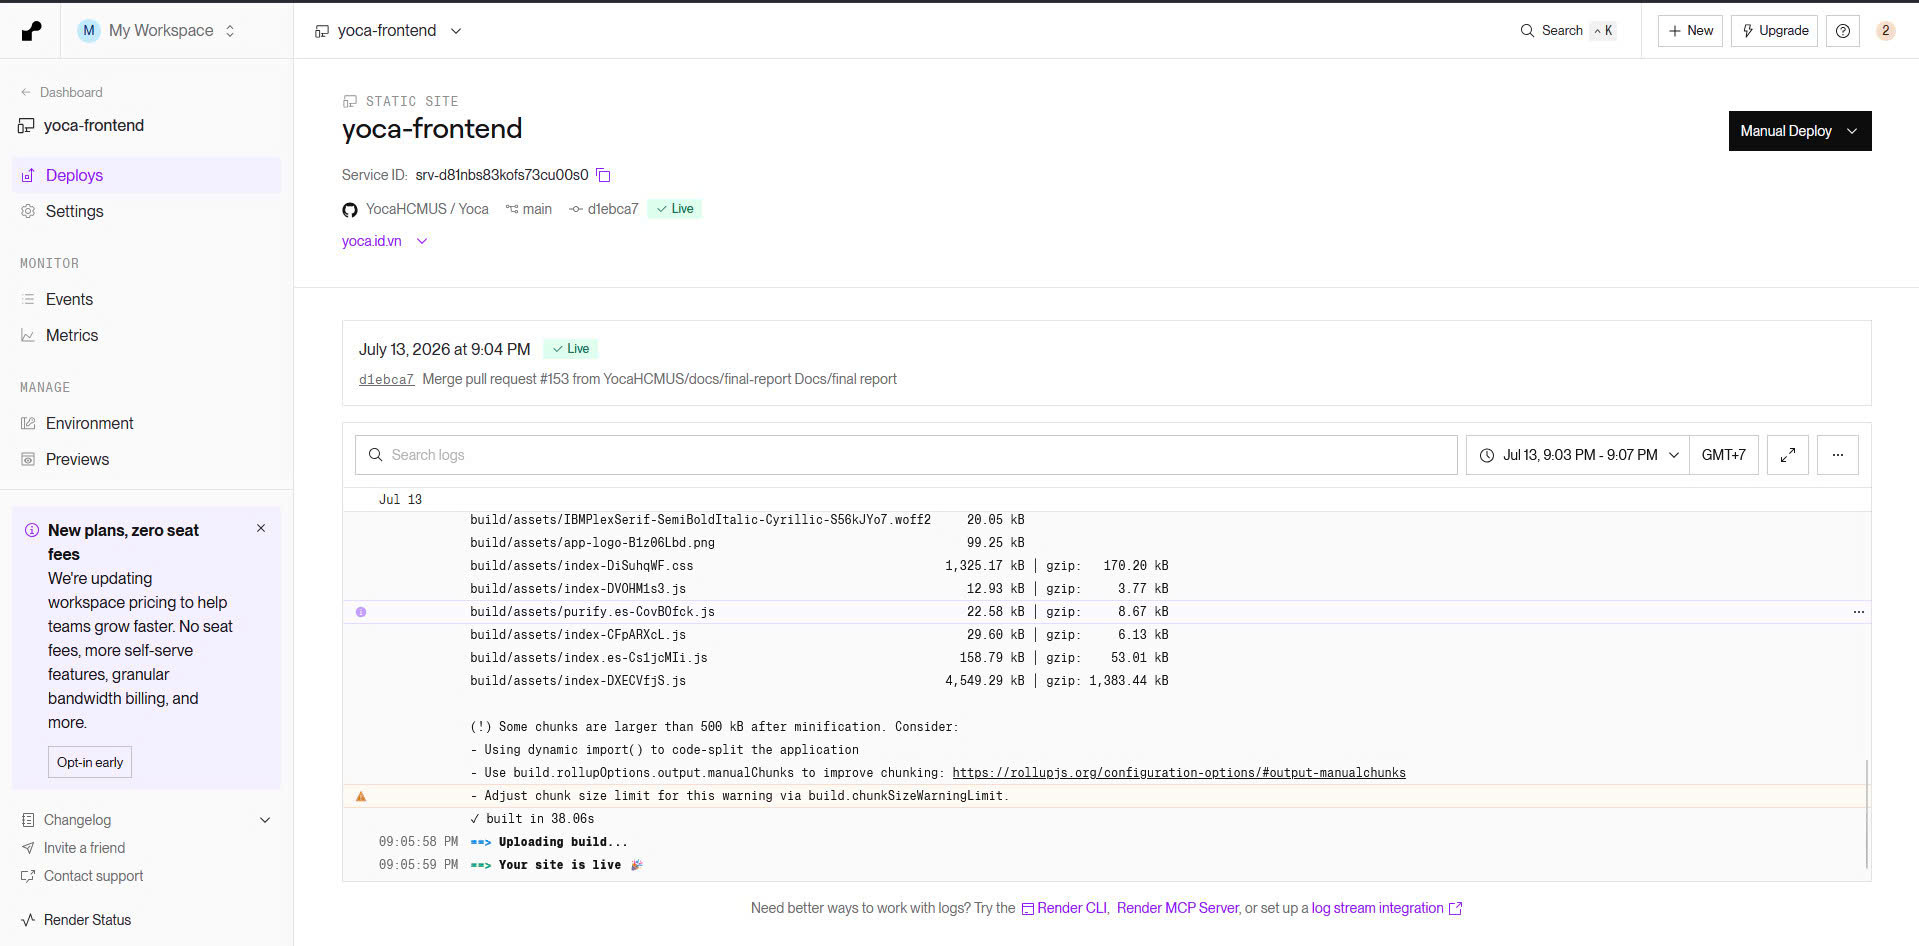
\includegraphics[width=0.95\textwidth]{images/chapter5/render-deployment-frontend.jpg}
    \caption{Render Static Site \texttt{yoca-frontend} ở trạng thái Live, phục vụ tại tên miền \texttt{yoca.id.vn}}
    \label{fig:render-deployment-frontend}
\end{figure}

\begin{figure}[H]
    \centering
    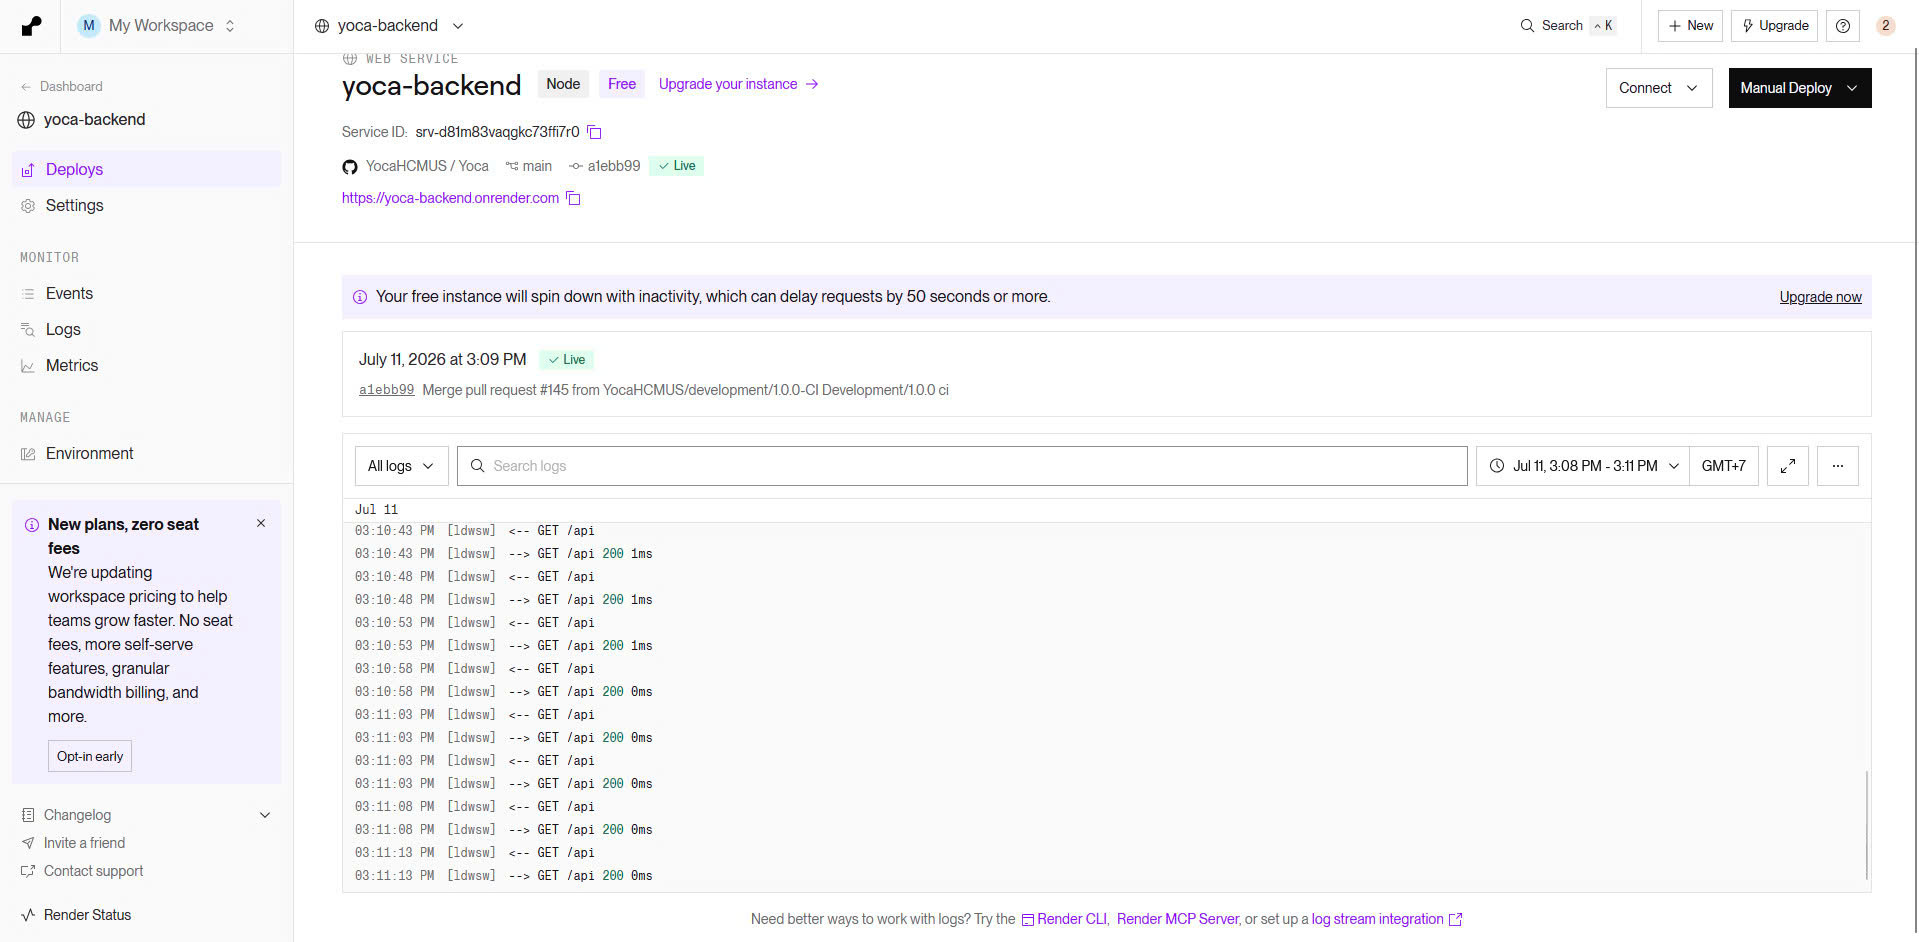
\includegraphics[width=0.95\textwidth]{images/chapter5/render-deployment-backend.jpg}
    \caption{Render Web Service \texttt{yoca-backend} ở trạng thái Live tại \texttt{yoca-backend.onrender.com}, log cho thấy các request \texttt{GET /api} thật trả về 200}
    \label{fig:render-deployment-backend}
\end{figure}


\section{Kết quả triển khai các chức năng cốt lõi}
\label{sec:ket_qua_trien_khai}
Các chức năng cốt lõi của Yoca đã được kết nối thành một chuỗi sử dụng liên tục. Người dùng có thể bắt đầu từ tìm kiếm hoặc tổng quan thị trường, đi sâu vào token và pool, phân tích ví và giao dịch, sau đó lưu đối tượng quan tâm hoặc thiết lập cảnh báo.

\subsection{Xác thực tài khoản}

Yoca hỗ trợ ba phương thức xác thực gồm đăng nhập bằng email, đăng nhập bằng Google và xác thực thông qua ví Solana, đáp ứng nhu cầu của nhiều nhóm người dùng trong hệ sinh thái blockchain.

Với phương thức email, người dùng có thể đăng ký tài khoản và đăng nhập bằng địa chỉ email cùng mật khẩu. Hệ thống cũng hỗ trợ luồng quên mật khẩu, cho phép người dùng đặt lại mật khẩu thông qua mã xác nhận được gửi qua email.

Đối với đăng nhập bằng Google, người dùng có thể xác thực nhanh mà không cần tạo tài khoản riêng.

Với xác thực bằng ví Solana, người dùng ký một thông điệp xác thực để chứng minh quyền sở hữu ví. Quá trình này không thực hiện giao dịch trên blockchain và chỉ được sử dụng để thiết lập phiên đăng nhập.

Giao diện xác thực được thiết kế dưới dạng hộp thoại, cho phép chuyển đổi linh hoạt giữa đăng nhập và đăng ký, đồng thời hỗ trợ hiển thị thông báo lỗi và tương thích với cả giao diện sáng và tối.

% CHÈN HÌNH: Modal xác thực với các phương thức đăng nhập bằng email, Google và ví Solana.

\subsection{Trang tổng quan thị trường}
\label{subsec:tong_quan_thi_truong}
Trang tổng quan thị trường của Yoca được thiết kế xoay quanh hoạt động giao dịch thực tế thay vì chỉ xếp hạng token theo vốn hóa, nhằm phản ánh trung thực hơn những gì đang diễn ra trên các sàn giao dịch phi tập trung.
Giao diện tổ chức dữ liệu thành sáu nhóm có thể chuyển đổi độc lập:
\begin{itemize}
    \item Trending: Token hoặc pool đang thu hút sự chú ý theo lượng tìm kiếm và hoạt động giao dịch.
    \item Top Volume/Transactions: Nhóm dẫn đầu theo khối lượng giao dịch hoặc số lần giao dịch.
    \item Gainers/Losers: Nhóm tăng hoặc giảm giá đáng chú ý trong khoảng thời gian quan sát.
    \item New Pairs: Các cặp giao dịch mới xuất hiện gần đây trên các sàn phi tập trung.
    \item Profitable Traders: Những nhà giao dịch đạt lợi nhuận hoặc chịu thua lỗ lớn nhất.
\end{itemize}

Bộ lọc thời gian cho phép người dùng quan sát dữ liệu Trending theo các cửa sổ 5 phút, 1 giờ, 6 giờ và 24 giờ. Nhóm Profitable Traders hỗ trợ khoảng quan sát 1 ngày, 7 ngày, 30 ngày và 90 ngày. Mỗi dòng dữ liệu hiển thị đầy đủ: tên token hoặc cặp giao dịch, vốn hóa thị trường, định giá pha loãng hoàn toàn (FDV), giá hiện tại, tuổi của pool, số giao dịch 24 giờ, khối lượng 24 giờ, biến động theo 5 phút, 1 giờ, 6 giờ và 24 giờ, cùng thanh khoản hiện có.

Người dùng có thể sắp xếp bảng theo bất kỳ cột nào và áp dụng bộ lọc theo khoảng thanh khoản, vốn hóa, khối lượng, số giao dịch, tuổi pool hoặc mức biến động. Việc chọn một token, pool hoặc địa chỉ nhà giao dịch từ danh sách sẽ điều hướng đến trang phân tích tương ứng, đảm bảo trang tổng quan không chỉ là nơi quan sát mà còn là điểm khởi đầu của quá trình nghiên cứu sâu hơn.
% CHÈN HÌNH: Trang tổng quan thị trường với các nhóm Trending, Top Volume/Transactions, Gainers/Losers, New Pairs và Profitable Traders.

\subsection{Tìm kiếm}
\label{subsec:tim_kiem}

Thanh tìm kiếm toàn cục là công cụ điều hướng trung tâm của hệ thống, hỗ trợ tra cứu đồng thời ba loại đối tượng: token, pool giao dịch và địa chỉ ví.

Mỗi kết quả kèm theo thông tin cơ bản tương ứng với từng loại đối tượng: token hiển thị ký hiệu, giá, biến động 24 giờ, vốn hóa thị trường, khối lượng và biểu đồ sparkline 7 ngày; pool hiển thị tên cặp, sàn giao dịch và các chỉ số thanh khoản; ví hiển thị địa chỉ và thông tin nhận diện. Người dùng có thể xem thông tin này ngay trong giao diện tìm kiếm mà không cần mở trang riêng.

Người dùng có thể điều khiển danh sách kết quả bằng bàn phím hoặc chuột. Khi lựa chọn một kết quả, hệ thống tự động điều hướng đến trang tổng quan token, trang chi tiết pool hoặc trang phân tích ví tương ứng.

% CHÈN HÌNH: Thanh tìm kiếm toàn cục với kết quả token, pool và ví kèm thông tin cơ bản.

\subsection{Trang tổng quan token}
\label{subsec:tong_quan_token}

Trang tổng quan token cung cấp bức tranh toàn diện về một token, bao gồm thông tin nhận diện, thống kê thị trường, biểu đồ giá và các phân tích chuyên sâu theo nhiều chiều dữ liệu.

Phần đầu trang hiển thị tên, ký hiệu, địa chỉ hợp đồng, ảnh đại diện và các liên kết chính thức khi có. Khu vực thống kê nhanh trình bày giá và biến động, giá cao/thấp trong 24 giờ, thứ hạng vốn hóa, vốn hóa thị trường, FDV, khối lượng giao dịch 24 giờ, ATH và ATL lịch sử.

Biểu đồ hỗ trợ ba chế độ: đường giá, đường vốn hóa và nến. Hai chế độ đường hỗ trợ các khoảng 24 giờ, 7 ngày, 30 ngày, 90 ngày và 1 năm. Biểu đồ nến sử dụng pool ưu tiên của token để phản ánh diễn biến giao dịch thực tế. Các sự kiện tin tức được đánh dấu trực tiếp trên trục thời gian; khi chọn một sự kiện, phần tóm lược và danh sách bài viết liên quan hiện ngay phía dưới mà không cần rời khỏi ngữ cảnh biến động giá.

Phần nội dung chuyên sâu được tổ chức thành nhiều thẻ:
\begin{itemize}
    \item Overview: giải thích các chỉ số về khối lượng, biến động, vốn hóa, nguồn cung lưu hành, FDV và khoảng cách hiện tại so với ATH/ATL.
    \item Holders: hiển thị danh sách địa chỉ nắm giữ lớn và biểu đồ phân bố nguồn cung theo bốn lớp: 10 ví lớn nhất, nhóm ví từ vị trí 11 đến 25, nhóm từ vị trí 26 đến 50, và phần còn lại. Cách phân lớp này giúp người dùng đánh giá mức độ tập trung nguồn cung một cách trực quan mà không cần đọc từng địa chỉ riêng lẻ.
    \item Tokenomics: trình bày cơ cấu phân bổ token, tỷ trọng từng nhóm, lượng token mở khóa tích lũy theo thời gian và các đợt mở khóa sắp tới.
    \item Investors: liệt kê các tổ chức hoặc cá nhân hậu thuẫn token, bao gồm vai trò, loại hình, quốc gia và mô tả.
    \item Markets: liệt kê các pool nổi bật theo sàn giao dịch, cặp, giá, biến động 24 giờ, khối lượng và thanh khoản. Lựa chọn một pool sẽ chuyển đến trang chi tiết pool tương ứng.
    \item News: tổng hợp bài viết từ nhiều nguồn RSS và kết quả tìm kiếm, phân biệt giữa tin tức chính thức và nội dung chỉ đề cập đến token trên web.
\end{itemize}

Khu vực quy đổi tỷ giá cho phép nhập một giá trị và xem ngay kết quả quy đổi sang nhiều đơn vị tiền tệ khác. Trợ lý AI được tích hợp trực tiếp trong trang, nhận bối cảnh token hiện tại làm đầu vào để hỗ trợ người dùng đặt câu hỏi phân tích.

Ngoài ra, trang token cũng cung cấp mục dữ liệu lịch sử, nơi giá đóng cửa, vốn hóa và khối lượng giao dịch được trình bày theo ngày dưới dạng bảng, sắp xếp mới nhất lên đầu. Người dùng chọn khoảng quan sát từ 7 ngày đến 1 năm và có thể tải thêm dữ liệu theo từng trang, phù hợp khi cần tra cứu giá trị tại một thời điểm cụ thể hoặc lấy số liệu thô cho phân tích bên ngoài.

% CHÈN HÌNH: Trang tổng quan token với biểu đồ giá/vốn hóa/nến và các thẻ Holders, Tokenomics, Investors.

\subsection{Trang chi tiết pool}

Trang chi tiết pool phục vụ việc phân tích token trong bối cảnh một cặp thanh khoản cụ thể. Trang này được tách biệt với trang tổng quan token nhằm phân biệt các chỉ số của toàn bộ token với các chỉ số chỉ áp dụng cho một pool giao dịch.

Người dùng có thể chuyển giữa các pool nổi bật của cùng một token thông qua bộ chọn pool. Mỗi lựa chọn hiển thị sàn giao dịch (DEX), tên cặp, địa chỉ pool, thanh khoản và khối lượng giao dịch trong 24 giờ, giúp việc so sánh giữa các pool trở nên thuận tiện.

Sau khi lựa chọn pool, hệ thống hiển thị khu vực thống kê với các chỉ số quan trọng như giá token, thanh khoản, vốn hóa, FDV, biến động giá, khối lượng mua và bán, tỷ lệ mua--bán, số lượng giao dịch, số nhà giao dịch, tỷ lệ nắm giữ của các holder lớn và nguồn cung.

Biểu đồ nến phản ánh diễn biến của cặp giao dịch đang được chọn. Đồng thời, khối tín hiệu biến động tổng hợp các thay đổi đáng chú ý trong dữ liệu gần đây, hỗ trợ người dùng nhanh chóng nhận biết các biến động nổi bật của thị trường.

Ngoài thông tin tổng quan, hệ thống còn cung cấp bảng giao dịch gần đây với các lệnh mua và bán, kèm theo số lượng token, giá, giá trị giao dịch, địa chỉ ví và mã giao dịch. Từ mỗi giao dịch, người dùng có thể mở phần chi tiết để theo dõi luồng chuyển tài sản trên blockchain.

Bên cạnh lịch sử giao dịch, tab Bubblemaps hiển thị biểu đồ phân bố holder, giúp trực quan hóa mối quan hệ giữa các ví nắm giữ token mà không cần rời khỏi trang. Điều này cho phép người dùng kết hợp quan sát hoạt động giao dịch với cấu trúc phân bố holder trong cùng một ngữ cảnh.

Cuối cùng, trang tiếp tục tích hợp tin tức liên quan, dữ liệu holder và trợ lý AI, giúp người dùng phân tích hoạt động của pool trong bối cảnh tổng thể của token.

% CHÈN HÌNH: Trang chi tiết pool với bộ chọn pool, thống kê thị trường và bảng giao dịch gần đây.

\subsection{Trang phân tích ví}
\label{subsec:phan_tich_vi}

Trang phân tích ví là một trong những chức năng trọng tâm của Yoca, cung cấp cái nhìn toàn diện về tài sản và hoạt động của một địa chỉ ví Solana. Phần đầu trang hiển thị thông tin ví cùng các thao tác như theo dõi, so sánh, chia sẻ, xuất dữ liệu và phân tích bằng AI.

Người dùng có thể lựa chọn khoảng thời gian 7, 30 hoặc 90 ngày để theo dõi các chỉ số tổng quan như tổng giá trị tài sản, số token đang nắm giữ hoặc đã giao dịch, tổng lãi/lỗ, lãi/lỗ đã thực hiện, lãi/lỗ chưa thực hiện, khối lượng giao dịch cùng số lần mua và bán.

Tiếp theo, hệ thống trực quan hóa dữ liệu thông qua biểu đồ số dư và biểu đồ PnL, giúp người dùng theo dõi sự thay đổi giá trị danh mục cũng như hiệu quả giao dịch theo từng giai đoạn.

Bên cạnh các biểu đồ, bảng danh mục tài sản liệt kê những token đang được nắm giữ cùng số dư, giá hiện tại và giá trị quy đổi. Từ đây, người dùng có thể chuyển trực tiếp đến trang tổng quan của từng token để tiếp tục phân tích.

Ngoài thông tin tổng quan, hệ thống còn cung cấp phần phân tích chi tiết cho từng vị thế token, bao gồm số dư hiện tại, lãi/lỗ, khối lượng mua và bán, giá trị ròng, số lần giao dịch cùng giá mua và giá bán trung bình. Lịch sử của từng token cũng có thể được xem theo nhiều khoảng thời gian khác nhau.

Hoạt động của ví được chia thành hai nhóm gồm các giao dịch swap và chuyển tài sản. Mỗi giao dịch đều hiển thị đầy đủ thông tin về tài sản, giá trị, thời gian, địa chỉ ví liên quan và mã giao dịch, đồng thời cho phép mở xem chi tiết mà không làm mất trạng thái hiện tại của trang.

Ngoài việc cung cấp dữ liệu giao dịch, hệ thống còn hỗ trợ gán nhãn ví, nhận diện tự động một số đặc trưng hành vi và tích hợp trợ lý AI để diễn giải hoạt động của ví dựa trên dữ liệu đang hiển thị. Kết quả AI đóng vai trò hỗ trợ phân tích và luôn được đặt cạnh các bảng hoặc biểu đồ tương ứng để người dùng dễ dàng đối chiếu với dữ liệu gốc.

Người dùng cũng có thể xuất dữ liệu của ví dưới nhiều định dạng khác nhau nhằm phục vụ nhu cầu lưu trữ hoặc phân tích bên ngoài.

% CHÈN HÌNH: Trang phân tích ví với tổng quan tài sản, biểu đồ số dư/PnL, danh mục và lịch sử hoạt động.

\subsection{Trang so sánh nhiều ví}
 
Trang so sánh cho phép quan sát từ hai đến nhiều địa chỉ ví trong cùng một hệ quy chiếu thời gian và thước đo, giúp nhận diện sự khác biệt về chiến lược, hiệu quả và mức độ rủi ro giữa các ví.

Người dùng thêm ví bằng cách nhập địa chỉ hoặc chọn từ danh sách ví đã theo dõi. Các biểu đồ được tổ chức thành ba nhóm chức năng:
\begin{itemize}
    \item Nhóm tổng quát: Xu hướng số dư nhiều ví theo thời gian, khối lượng giao dịch tổng, phân bố khối lượng và khối lượng trung bình trên mỗi giao dịch.
    \item Nhóm tài sản: Phân bố danh mục tài sản theo ví và tỷ lệ stablecoin của từng ví.
    \item Nhóm rủi ro và hiệu quả: PnL theo cửa sổ thời gian, tỷ lệ giao dịch có lãi và mức suy giảm tài sản tối đa (drawdown).
\end{itemize}

Mỗi biểu đồ có thể được đưa vào ngữ cảnh của trợ lý AI để đặt câu hỏi trực tiếp về dữ liệu đang hiển thị. Người dùng cũng có thể mở lại trang phân tích riêng của từng ví hoặc xuất toàn bộ phần so sánh sang định dạng PDF.

\subsection{Trang cảnh báo và theo dõi ví}

Trang cảnh báo yêu cầu người dùng đăng nhập và cung cấp cơ chế theo dõi ví theo thời gian thực thông qua tích hợp webhook Helius.

Quản lý danh sách ví theo dõi: Người dùng thêm địa chỉ ví cần theo dõi và đặt nhãn phân biệt. Khi một ví được thêm hoặc xóa khỏi danh sách, hệ thống tự động đồng bộ cấu hình với Helius Webhook: các địa chỉ được phân phối vào các nhóm webhook (shards) theo giới hạn 25 địa chỉ mỗi shard. Quá trình đồng bộ tạo, cập nhật hoặc xóa shard phù hợp để luôn phản ánh đúng danh sách hiện tại mà không yêu cầu người dùng thao tác thủ công.

Mỗi quy tắc cảnh báo được tạo qua hai bước rõ ràng. Ở bước đầu (cấu hình điều kiện), người dùng chỉ định:
\begin{itemize}
    \item Ví cần áp dụng quy tắc;
    \item Loại hoạt động kích hoạt: swap, chuyển tài sản hoặc tất cả;
    \item Khoảng giá trị tối thiểu và tối đa;
    \item Đơn vị giá trị: USD hoặc SOL;
    \item Kiểu kích hoạt: một lần (one-shot) hoặc lặp lại (recurring);
    \item Thời điểm hết hạn của quy tắc.
\end{itemize}

Ở bước thứ hai (cấu hình thông báo), người dùng chọn kênh nhận thông báo. Theo mặc định, thông báo được gửi đến email đã đăng ký. Người dùng có thể chỉ định email riêng hoặc URL Discord webhook cho từng quy tắc. Ngoài ra, người dùng đặt tên quy tắc và xem trước nội dung thông báo sẽ nhận được.

\begin{figure}[H]
    \centering
    \begin{minipage}{0.47\textwidth}
        \centering
        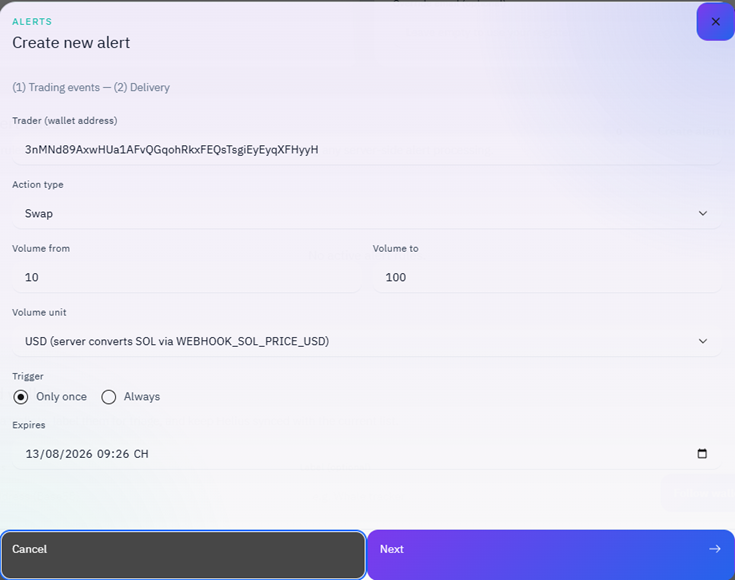
\includegraphics[width=\textwidth]{images/chapter5/alert-config-1.png}\\[3pt]
        {\small (a) Bước 1: điều kiện kích hoạt}
    \end{minipage}
    \hfill
    \begin{minipage}{0.47\textwidth}
        \centering
        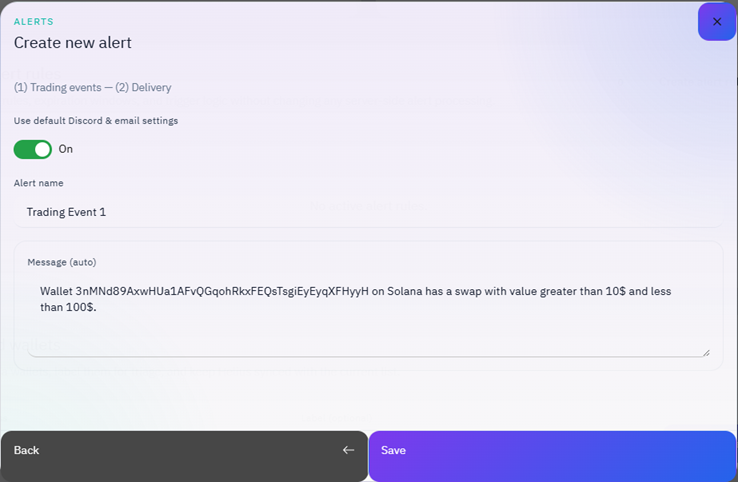
\includegraphics[width=\textwidth]{images/chapter5/alert-config-2.png}\\[3pt]
        {\small (b) Bước 2: kênh nhận và xem trước nội dung}
    \end{minipage}
    \caption{Tạo một alert rule thật: theo dõi swap của một ví trong khoảng giá trị 10--100 USD}
    \label{fig:alert-config}
\end{figure}

Danh sách quy tắc hiển thị ví, loại hoạt động, khoảng giá trị, kiểu kích hoạt và thời hạn; từ đó người dùng có thể tắt hoặc xóa quy tắc bất kỳ lúc nào.

Sau khi ít nhất một kênh gửi thành công, hệ thống ghi Alert History theo đúng tài khoản. Mỗi bản ghi giữ nội dung, mức độ, transaction signature, ví liên quan, thời điểm và kết quả email/Discord. Người dùng có thể xem lịch sử theo thứ tự mới nhất, đánh dấu đã đọc/chưa đọc hoặc đánh dấu toàn bộ; khóa idempotency ngăn webhook retry tạo thông báo trùng.

\begin{figure}[H]
    \centering
    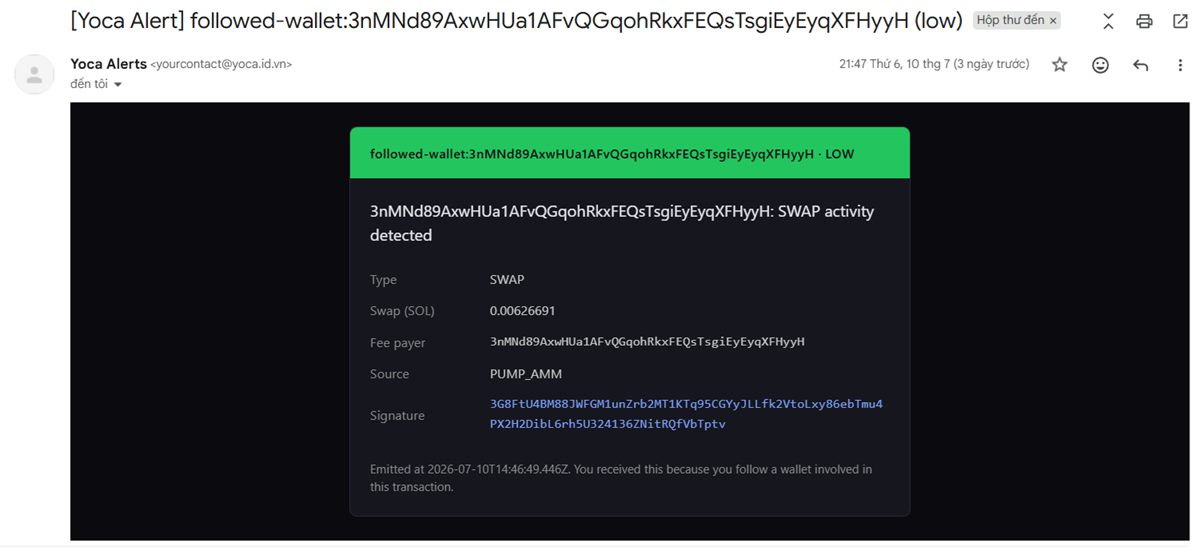
\includegraphics[width=0.85\textwidth]{images/chapter5/alert-delivery-email.png}
    \caption{Email cảnh báo nhận được thật sau khi rule ở Hình~\ref{fig:alert-config} kích hoạt: sự kiện SWAP trên ví theo dõi, kèm nguồn, số lượng và transaction signature}
    \label{fig:alert-delivery-email}
\end{figure}

Hai hình trên xác nhận luồng end-to-end (tạo rule -- Helius phát sinh sự kiện -- gửi thành công) đã chạy được trên môi trường thật. % TODO(SCREENSHOT-OPTIONAL): nếu có, bổ sung thêm ảnh giao diện Alert History (danh sách, trạng thái đã đọc/chưa đọc) để minh họa phần lưu trữ phía trong ứng dụng; không bắt buộc vì email đã là bằng chứng delivery độc lập.

\subsection{Trang hồ sơ cá nhân}

Trang hồ sơ cá nhân là trung tâm quản lý tài sản và tùy chỉnh trải nghiệm, được tổ chức thành các thẻ chức năng liên kết chặt chẽ với nhau.

Bắt đầu từ thẻ Portfolio (Overview), người dùng thiết lập danh sách các ví cần theo dõi. Thẻ này cung cấp cái nhìn nhanh về tổng giá trị của từng ví, cho phép thêm mới hoặc gỡ bỏ các ví không còn nhu cầu giám sát. 

Thẻ Dashboard là nơi tổng hợp toàn bộ dữ liệu từ các ví của người dùng thành một bảng điều khiển trung tâm duy nhất. Chức năng này cung cấp bức tranh toàn cảnh về sức khỏe tài chính thông qua các biểu đồ phân tích chuyên sâu được tạo sẵn, như phân bố khối lượng giao dịch, ma trận cơ cấu tài sản, và đối sánh lãi/lỗ (PnL). Nhờ đó, người dùng nắm bắt được hiệu suất của toàn bộ danh mục đầu tư mà không cần thao tác thiết lập phức tạp.

Bên cạnh tài sản cá nhân, người dùng có thể theo dõi thị trường thông qua thẻ Watchlist. Thẻ này hoạt động như một sổ tay lưu trữ các token và ví tiềm năng đang trong tầm ngắm, giúp dễ dàng mở nhanh để xem biến động hoặc chỉnh sửa nhãn phân loại.

Tiếp theo là thẻ Subscriptions, thẻ này giúp quản lý gói dịch vụ và lịch sử thanh toán minh bạch. Hệ thống hỗ trợ thanh toán qua thẻ ngân hàng hoặc bằng tiền mã hóa. Khi thanh toán bằng Solana, giao dịch chuyển tiền từ ví người dùng sẽ được máy chủ tự động truy xuất và xác minh nghiêm ngặt trên chuỗi khối (địa chỉ nhận, số tiền, trạng thái) trước khi cấp quyền dịch vụ.

Cuối cùng, mọi thiết lập định danh và bảo mật được quản lý tập trung tại thẻ Settings. Tại đây, người dùng có thể tùy chỉnh tên hiển thị, theo dõi và liên kết các phương thức đăng nhập đa dạng (như Email, tài khoản Google hoặc ví Solana). Thẻ này cũng cho phép thay đổi mật khẩu định kỳ hoặc thực hiện quy trình xóa tài khoản an toàn với bước xác nhận bổ sung, đảm bảo người dùng luôn có toàn quyền kiểm soát dữ liệu cá nhân của mình.

\subsection{Mô-đun phát hiện dấu hiệu wash trading}

Mô-đun phát hiện dấu hiệu wash trading hỗ trợ nhận diện các mẫu giao dịch có khả năng tạo khối lượng giả thông qua phân tích quan hệ giữa các ví trên blockchain. Đây là chức năng bổ sung cho các chỉ số thị trường truyền thống, giúp người dùng quan sát hành vi giao dịch ở mức độ sâu hơn.

Người dùng nhập địa chỉ mint của token, ký hiệu token và lựa chọn khoảng thời gian phân tích 24 giờ, 7 ngày hoặc 30 ngày. Từ dữ liệu giao dịch thu thập được, hệ thống xây dựng đồ thị ví--giao dịch và tính toán điểm rủi ro dựa trên nhiều đặc trưng, bao gồm:

\begin{itemize}
    \item Chu trình giao dịch (circular patterns);
    \item Tính đều đặn về thời gian (time regularity);
    \item Mức tương đồng về số lượng giao dịch (amount similarity);
    \item Giao dịch tự quay lại (self-loop);
    \item Vai trò của ví trung tâm (hubness);
    \item Tín hiệu bất thường về khối lượng (volume anomaly).
\end{itemize}

Sau khi phân tích hoàn tất, hệ thống hiển thị các chỉ số tổng hợp như tổng số giao dịch, số lượng ví tham gia, khối lượng wash trading ước tính, số ví đáng ngờ, số cụm giao dịch vòng và độ tin cậy của kết quả phân tích.

Bên cạnh các chỉ số thống kê, đồ thị ví--giao dịch được sử dụng để trực quan hóa mối quan hệ giữa các ví. Người dùng có thể phóng to, thu nhỏ, di chuyển đồ thị hoặc lựa chọn từng ví để xem các đặc trưng nổi bật và điểm rủi ro tương ứng. Giao diện cũng hỗ trợ chuyển đổi giữa các cấu hình thuật toán GCN, GAT và GraphSAGE nhằm so sánh kết quả phân tích theo các mô hình khác nhau.

Ngoài kết quả phân tích, hệ thống tích hợp trợ lý AI để diễn giải các dấu hiệu được phát hiện dựa trên bối cảnh của đồ thị và các chỉ số đã tính toán. Phần giải thích luôn được hiển thị cùng với dữ liệu nguồn, giúp người dùng dễ dàng đối chiếu và sử dụng kết quả như một tín hiệu hỗ trợ đánh giá, thay vì kết luận độc lập về hành vi gian lận.

% CHÈN HÌNH: Mô-đun wash trading với đồ thị ví-giao dịch, chỉ số tổng hợp và phần giải thích rủi ro.

\section{Giải quyết các thách thức kỹ thuật}
\label{sec:giai_quyet_thach_thuc}

\subsection{Xử lý giới hạn truy vấn và điều phối khóa truy cập}
Các nhà cung cấp dữ liệu đều áp dụng giới hạn về số lượng yêu cầu trong một khoảng thời gian nhất định. Trong khi đó, một thao tác như mở trang phân tích ví có thể đồng thời yêu cầu nhiều dữ liệu từ nhiều endpoint và nhiều nhà cung cấp khác nhau, dễ dẫn đến lỗi HTTP 429 và làm gián đoạn quá trình tải dữ liệu. 

Để giải quyết vấn đề này, Yoca xây dựng lớp điều phối \texttt{ThrottledQueue} riêng cho từng nhà cung cấp nhằm giới hạn số lượng yêu cầu đồng thời, thực hiện thử lại với khoảng chờ tăng dần khi gặp lỗi tạm thời và tuân theo thời gian chờ do nhà cung cấp trả về. Bên cạnh đó, cơ chế gộp yêu cầu (request coalescing) hợp nhất các yêu cầu giống nhau phát sinh đồng thời thành một lần gọi duy nhất, giúp giảm số lượng truy vấn không cần thiết. 

Đối với các dịch vụ sử dụng nhiều khóa API, hệ thống luân phiên sử dụng các khóa để phân tán tải và hạn chế vượt quá giới hạn của từng khóa. Đồng thời, các loại lỗi như giới hạn truy vấn, lỗi mạng và lỗi dữ liệu được xử lý theo các chiến lược khác nhau nhằm duy trì khả năng cung cấp dữ liệu ngay cả khi một số nguồn gặp sự cố. 

Nhờ đó, hệ thống duy trì được khả năng phản hồi ổn định, giảm đáng kể số lượng lỗi do vượt quá giới hạn truy vấn và tối ưu việc sử dụng tài nguyên của các nhà cung cấp dữ liệu.

\subsection{Tái sử dụng bộ đệm theo khoảng thời gian}

Dữ liệu lịch sử ví thường được truy vấn theo các khoảng thời gian chồng lấn. Nếu mỗi lần thay đổi khoảng thời gian đều tải lại toàn bộ dữ liệu, hệ thống sẽ phát sinh nhiều truy vấn lặp, làm tăng thời gian phản hồi và tiêu tốn tài nguyên. 

Để khắc phục vấn đề này, Yoca áp dụng cơ chế \textit{partial-range cache reuse}, trong đó dữ liệu giao dịch và phạm vi thời gian đã đồng bộ được lưu đồng thời trong bộ đệm. Khi nhận yêu cầu mới, hệ thống chỉ xác định và truy xuất phần dữ liệu còn thiếu, sau đó hợp nhất với dữ liệu hiện có dựa trên chữ ký giao dịch để loại bỏ các bản ghi trùng lặp. 

Cơ chế này cũng được áp dụng cho dữ liệu biểu đồ token. Nhờ chỉ đồng bộ phần dữ liệu còn thiếu, hệ thống giảm đáng kể số lần gọi đến nhà cung cấp, đồng thời cải thiện tốc độ phản hồi khi người dùng chuyển đổi giữa các khoảng thời gian. 

Qua đó, dữ liệu được tái sử dụng hiệu quả hơn, góp phần nâng cao hiệu năng của hệ thống và giảm tải cho các dịch vụ bên ngoài.

\subsection{Định giá USD lịch sử cho danh mục ví}
Việc xác định giá trị danh mục tại một thời điểm trong quá khứ không thể sử dụng giá hiện tại của token, vì điều này có thể tạo ra sai lệch lớn so với giá trị thực tế. 

Để giải quyết bài toán này, Yoca trước hết dựng lại số dư của từng token tại thời điểm cần quan sát từ lịch sử các giao dịch chuyển và giao dịch swap. Sau đó, hệ thống tra cứu mức giá lịch sử gần nhất của từng token để tính giá trị quy đổi sang USD. 

Trong trường hợp không có dữ liệu giá lịch sử, hệ thống sử dụng giá hiện tại khi dữ liệu thị trường vẫn đáng tin cậy. Nếu vẫn không thể xác định được mức giá phù hợp, token sẽ không được cộng vào tổng giá trị USD nhưng vẫn được giữ trong danh mục, tránh đưa ra các giá trị suy đoán có thể gây hiểu nhầm. 

Cách tiếp cận này giúp kết quả định giá phản ánh sát hơn giá trị danh mục tại từng thời điểm, đồng thời đảm bảo tính nhất quán và độ tin cậy của các chỉ số tài chính trong hệ thống.

\subsection{Chuẩn hóa dữ liệu từ nhiều nguồn}

Các nhà cung cấp dữ liệu thường sử dụng những định dạng và cấu trúc khác nhau để biểu diễn cùng một loại thông tin. Nếu xử lý trực tiếp dữ liệu thô, các chức năng phía trên sẽ phải phụ thuộc vào từng nhà cung cấp và khó đảm bảo tính nhất quán. 

Để khắc phục điều này, Yoca thực hiện chuẩn hóa dữ liệu trước khi lưu trữ và trước khi hiển thị. Các giao dịch được quy về các hành động chuẩn như swap, gửi và nhận; trong khi dữ liệu thị trường và tin tức cũng được chuyển về một mô hình thống nhất trước khi sử dụng. 

Nhờ đó, toàn bộ các mô-đun trong hệ thống có thể xử lý dữ liệu theo cùng một cấu trúc, giảm sự phụ thuộc vào từng nhà cung cấp và tạo thuận lợi cho việc mở rộng hệ thống trong tương lai.

\subsection{Duy trì tính giải thích của kết quả AI}

Các mô hình AI khó khai thác hiệu quả dữ liệu blockchain ở dạng thô, đồng thời kết quả sinh ra cần có khả năng đối chiếu với dữ liệu nguồn để đảm bảo tính minh bạch. 

Để giải quyết vấn đề này, trước khi gửi yêu cầu đến mô hình AI, Yoca xây dựng một bối cảnh có cấu trúc gồm các chỉ số tổng hợp, giao dịch tiêu biểu, khoảng thời gian phân tích và các bằng chứng liên quan. Việc này giúp mô hình tập trung vào những thông tin quan trọng thay vì xử lý toàn bộ dữ liệu blockchain.

Sau khi AI tạo kết quả, phần diễn giải luôn được hiển thị cùng với bảng dữ liệu hoặc biểu đồ tương ứng để người dùng dễ dàng đối chiếu. Đối với mô-đun wash trading, kết quả được liên kết trực tiếp với các đặc trưng và các ví đáng ngờ; trong khi ở các trang phân tích ví và token, AI chỉ diễn giải dữ liệu của đối tượng đang được quan sát. 

Qua đó, hệ thống vừa tận dụng được khả năng diễn giải của AI, vừa đảm bảo người dùng luôn có thể kiểm chứng các nhận định dựa trên dữ liệu gốc, giúp tăng tính minh bạch và độ tin cậy của kết quả phân tích.

\section{Kết quả kiểm thử và đánh giá hệ thống}
\label{sec:kiem_thu_danh_gia}

Hoạt động kiểm thử được thực hiện nhằm xác nhận các chức năng của Yoca vận hành đúng theo yêu cầu, các thành phần có thể phối hợp ổn định và dữ liệu hiển thị duy trì được tính nhất quán. Bên cạnh kiểm thử chức năng, quá trình đánh giá tập trung vào hiệu quả của cơ chế bộ đệm, khả năng xử lý lỗi từ nhà cung cấp, độ trễ cảnh báo và thời gian phân tích đồ thị giao dịch.

\subsection{Môi trường và dữ liệu kiểm thử}

\subsection{Kết quả kiểm thử chức năng}

\subsection{Kết quả kiểm thử tích hợp}

\subsection{Đánh giá hiệu năng và hiệu quả bộ đệm}

\subsection{Kết quả chạy test và vấn đề còn tồn tại}

Ngày 12/07/2026, nhóm chạy hai lệnh \texttt{npm test -w client -- --run} và \texttt{npm test -w server} trên source hiện tại. Kết quả được trình bày trong Bảng~\ref{tab:test_results}; đây là số liệu của đúng lần chạy này, không phải coverage hay tỷ lệ ổn định dài hạn.

\begin{table}[H]
\centering
\small
\begin{tabularx}{\textwidth}{|L{2.5cm}|C{2.2cm}|C{2.2cm}|X|}
\hline
\textbf{Suite} & \textbf{Test file} & \textbf{Test case} & \textbf{Kết quả} \\
\hline
Client & 16/16 đạt & 178/178 đạt & Các test component, payment, profile, chart interaction, utility và Alert History API đều đạt trong lần chạy ngày 12/07/2026. \\
\hline
Server & 29/29 đạt & 204/204 đạt & Các test auth/entitlement, payment, alert/webhook/history, AI guardrail và prompt injection, Wallet, provider mapping, pagination cùng route/service đều đạt trong lần chạy ngày 12/07/2026. \\
\hline
\end{tabularx}
\caption{Kết quả chạy test trên source hiện tại}
\label{tab:test_results}
\end{table}

Kết quả cho thấy repository đã có nền tảng kiểm thử đáng kể và hai suite hiện đều ở trạng thái xanh. Trong đợt rà cuối, nhóm chúng em sửa các expectation đã lỗi thời sau thay đổi localization/theme, thống nhất contract lỗi upstream và bổ sung test cho Alert History, provider mapper cùng cursor/offset pagination. Kết quả này đủ để dùng test làm một cổng kiểm tra trong CI, nhưng chưa thay thế E2E trên môi trường triển khai hay đánh giá tải thực tế.

\subsection{Đánh giá và phạm vi kiểm thử còn thiếu}

Các test hiện tại chưa đo đầy đủ cache hit/miss trên môi trường có PostgreSQL thật, chưa gọi provider thật theo contract regression và chưa chạy toàn bộ user journey trong browser. Repository cũng chưa cung cấp load test, benchmark có thể lặp lại, staging ổn định hay số liệu về độ trễ cảnh báo. Vì vậy, chương này không đưa ra con số cải thiện hiệu năng hoặc khẳng định độ ổn định toàn hệ thống.

Phạm vi hoàn thiện vừa đủ gồm bốn lớp: unit test cho normalizer và phép tính; provider contract test bằng response fixture đã ẩn dữ liệu nhạy cảm; route/service test cho fresh/stale/error và các status 200, 400, 429, 500, 502, invalid JSON, schema mismatch; cuối cùng là smoke test cho hành trình demo. Suite tự động hiện đã xanh; phần còn lại trước bản nộp là chạy smoke test trên database và môi trường deploy thật, đặc biệt với delivery và lịch sử cảnh báo.

\section{Tổng kết chương}
\label{sec:tong_ket_ch4}

Chương 4 đã trình bày quá trình triển khai thực nghiệm hệ thống Yoca, bao gồm môi trường vận hành, tích hợp các nguồn dữ liệu, quy trình tích hợp và triển khai mã nguồn, cùng kết quả hiện thực các nhóm chức năng cốt lõi. Các chức năng được tổ chức thành luồng sử dụng thống nhất, từ khám phá thị trường, phân tích token và pool đến theo dõi ví, giao dịch, cảnh báo và hỗ trợ diễn giải bằng AI.

Chương cũng làm rõ những giải pháp được áp dụng để xử lý các thách thức của dữ liệu blockchain, gồm giới hạn truy vấn, dữ liệu lịch sử chồng lấn, định giá danh mục trong quá khứ và sự khác biệt giữa các nhà cung cấp. Trong đó, mô-đun phát hiện dấu hiệu wash trading thể hiện khả năng kết hợp phân tích đồ thị, chấm điểm rủi ro, trực quan hóa quan hệ giữa các ví và giải thích kết quả dựa trên dữ liệu nguồn.

Kết quả kiểm thử cho thấy các thành phần chính phối hợp đúng theo luồng nghiệp vụ, dữ liệu được chuẩn hóa nhất quán và hệ thống duy trì khả năng vận hành trong các kịch bản được đánh giá. Những kết quả này là cơ sở để Chương 5 tổng kết các đóng góp của đề tài, phân tích những giới hạn khách quan và đề xuất các hướng phát triển tiếp theo cho Yoca.

\chapter{Kết luận và hướng phát triển}
\label{Chapter6}

Chương này tổng kết những gì Yoca đã đạt được sau quá trình phát triển, đồng thời nhìn nhận các giới hạn còn tồn tại. Thay vì lặp lại danh sách chức năng của Chương 5, nội dung tập trung vào giá trị của luồng phân tích, các quyết định kỹ thuật có khả năng tái sử dụng và những công việc cần ưu tiên nếu hệ thống tiếp tục được hoàn thiện.

\section{Kết quả và đóng góp chính}

Yoca đã hình thành một luồng phân tích liên tục từ Market Overview đến Token Pool, Token Overview, Wallet, User và các chức năng AI. Điểm quan trọng của luồng này không nằm ở số lượng trang, mà ở việc người dùng có thể đi từ biến động thị trường đến pool cụ thể, quan sát ví tham gia, kiểm tra giao dịch và quay lại dữ liệu nguồn mà không phải tự ghép nhiều công cụ rời rạc. Các chức năng tài khoản, watchlist, nhãn ví, subscription và cảnh báo bổ sung lớp cá nhân hóa cho quá trình sử dụng.

Đóng góp kỹ thuật đầu tiên là lớp dữ liệu nhiều provider được đặt sau một hợp đồng nội bộ. CoinGecko, Birdeye, Helius, Mobula, Zerion và Moralis được chọn theo miền thay vì tạo fallback tràn lan. Response bên ngoài được kiểm tra bằng Zod trước khi đi vào nghiệp vụ; Hono RPC và TypeScript giữ hợp đồng giữa client với server; PostgreSQL và Drizzle quản lý dữ liệu nền cùng các read model cache. Cách tổ chức này không loại bỏ sự phụ thuộc provider, nhưng giới hạn nơi sự khác biệt về schema và semantics lan vào hệ thống.

Đóng góp thứ hai là cách xem cache như một phần của thiết kế dữ liệu. Snapshot có thể dùng TTL, còn lịch sử transfer, swap và transaction cần coverage metadata để xác định khoảng đã tải. Các bảng được tách theo nguồn và nhịp cập nhật nhằm tránh việc một hàng chỉ hoàn chỉnh sau nhiều lần gọi API. Quá trình migration Wallet cũng cho thấy khả năng thay thế tăng dần: Mobula hiện cung cấp các chỉ số phân tích và lịch sử tổng tài sản, Zerion giữ lịch sử theo token, còn Helius tiếp tục phục vụ portfolio, webhook và transaction detail.

Đối với phân tích ví, nhóm chúng em đã đi từ thử nghiệm tự giải mã Enhanced Transactions và heuristic balance change đến một phạm vi thực tế hơn. PnL tổng hợp được đọc từ dữ liệu Mobula đã kiểm tra và cache; đường PnL theo ngày được phân biệt rõ với realized PnL, dựa trên biến động tổng tài sản sau khi trừ dòng tiền ròng. Việc ghi rõ nguồn, kỳ phân tích và độ phủ giúp kết quả có thể được diễn giải đúng giới hạn thay vì được xem như sổ cái kế toán tuyệt đối.

Yoca còn kết hợp dữ liệu định lượng với lớp diễn giải AI. Dữ liệu token, ví và giao dịch được chuẩn bị thành ngữ cảnh có cấu trúc trước khi gửi đến mô hình. Kết quả được đặt cạnh bảng, biểu đồ hoặc giao dịch liên quan để người dùng có cơ sở đối chiếu. Mô-đun wash trading mở rộng cách quan sát từ từng bản ghi sang quan hệ đồ thị và các tín hiệu như chu trình, hubness, mức tương đồng và bất thường khối lượng; đây là tín hiệu hỗ trợ đánh giá, không phải kết luận gian lận tự động.

Về khả năng tiếp cận, lớp localization dùng chung hỗ trợ tiếng Anh, tiếng Việt, định dạng số/ngày giờ và quy đổi USD sang VND tại lớp trình bày. Cấu trúc translation key và biến nội suy được kiểm tra trong lúc phát triển. Đây là phần đóng góp gắn trực tiếp với mục tiêu giúp người dùng Việt Nam tiếp cận dữ liệu blockchain quen thuộc hơn, dù một số component cũ vẫn chưa được bản địa hóa hoàn toàn.

\section{Giới hạn còn tồn tại}

Giới hạn lớn nhất của hệ thống là chất lượng và tính liên tục của dữ liệu vẫn phụ thuộc vào provider. Quota, giá gói, phạm vi lịch sử, trường nullable và cách phân loại token có thể thay đổi. Kinh nghiệm chuyển từ Birdeye sang Mobula--Zerion cho thấy thay provider không chỉ sửa endpoint mà còn ảnh hưởng adapter, cache, schema và cách giải thích chỉ số. Một số read model, đặc biệt \texttt{wallet\_analyses}, vẫn mang hình dạng gần với provider vì được xây dựng trong giai đoạn migration gấp.

Kết quả phân tích tài chính cũng có giới hạn về độ phủ. Token mới hoặc ít thanh khoản có thể thiếu giá lịch sử; transaction phức tạp có thể không được lớp Enhanced Transactions mô tả đầy đủ; PnL theo balance phụ thuộc vào giá trị tổng tài sản và transfer có giá USD. Nhãn ví, AI và tín hiệu wash trading đều cần được xem cùng dữ liệu nguồn, không nên sử dụng như nhận định chắc chắn về chủ thể hay hành vi.

Giao diện hiện chưa có một design system được áp dụng trọn vẹn. Carbon, SCSS module, utility class và component tự xây vẫn cùng tồn tại. Landing, Market và Wallet đã được đổi mới nhiều hơn, trong khi một số component Token/Pool còn style và behavior cũ. Localization cũng còn chuỗi hard-code. Vấn đề này liên quan đến component contract, accessibility và trạng thái loading/error/empty, không chỉ là màu sắc.

Phạm vi kiểm thử và vận hành chưa đủ để khẳng định hệ thống ổn định ở quy mô lớn. Lần chạy gần nhất còn 17 client test và 8 server test thất bại; chưa có E2E đầy đủ, load test, benchmark cache trên PostgreSQL thật hoặc staging ổn định. CI/CD đang được phát triển ở nhánh khác và chưa được xem là kết quả hoàn thành. Alert History mới có schema và thiết kế dự kiến; luồng ghi sau delivery, ownership API, read state và chống trùng vẫn là hạng mục bắt buộc phải triển khai.

\section{Hướng phát triển}

Ưu tiên đầu tiên là khép lại các contract đang không thống nhất. Nhóm cần quyết định rõ cách biểu diễn lỗi provider, sửa đường Zerion balance để phân biệt response rỗng, malformed JSON và upstream failure, sau đó đưa các fixture này vào contract regression test. Test suite phải trở về trạng thái xanh trước khi CI trở thành cổng merge. Bước tiếp theo là bổ sung smoke test cho user journey chính và E2E chọn lọc cho auth, Wallet, payment và alert; số liệu hiệu năng chỉ được đưa ra sau khi có benchmark lặp lại được.

Ở lớp tích hợp, hệ thống cần bổ sung observability cho thời gian phản hồi, tỷ lệ lỗi, retry, quota và cache hit/miss theo provider. Retry phải có giới hạn; circuit breaker và stale-data policy cần được định nghĩa cho những endpoint quan trọng. Adapter nội bộ và read model nên tiếp tục giảm coupling với response provider, đặc biệt ở Wallet, nhưng không nên refactor đồng loạt khi consumer cũ vẫn hoạt động.

Ở giao diện, hướng phát triển phù hợp là thống nhất design token, quy định component contract và trạng thái dữ liệu, sau đó migration theo màn hình ưu tiên thay vì thay toàn bộ thư viện một lần nữa. Cùng lúc đó, nhóm cần loại bỏ chuỗi hard-code, bổ sung kiểm tra parity locale và hoàn thiện bộ ảnh chức năng bằng dữ liệu demo ổn định.

Alert History cần được hoàn thiện end-to-end: ghi sự kiện sau delivery, giới hạn theo user, đánh dấu đã đọc và chống duplicate khi webhook retry. Khi nhánh CI/CD hoàn tất, báo cáo và quy trình vận hành phải được cập nhật bằng workflow thật, bao gồm quản lý secret, migration và smoke check sau deployment.

Về dài hạn, mô-đun wash trading có thể được đánh giá trên tập dữ liệu đã kiểm chứng và kết hợp thêm biến động giá, thanh khoản cùng hành vi qua nhiều pool. AI có thể tăng khả năng dẫn chứng bằng cách liên kết từng nhận định với giao dịch hoặc vùng biểu đồ cụ thể. Những mở rộng này chỉ có ý nghĩa khi nền tảng dữ liệu, kiểm thử và quan sát vận hành đã đủ tin cậy.

Nhìn chung, Yoca đã tạo được nền tảng cho một sản phẩm phân tích Solana có luồng sử dụng rõ ràng và có chủ đích đối với người dùng Việt Nam. Kết quả quan trọng nhất của đề tài là kinh nghiệm tổ chức dữ liệu nhiều nguồn, nhận diện giới hạn của việc tự giải mã, điều chỉnh kiến trúc khi provider thay đổi và giữ cho kết quả phân tích có thể đối chiếu. Các giới hạn còn lại được xem là điểm xuất phát cụ thể cho giai đoạn hoàn thiện tiếp theo, thay vì được che khuất bằng những khẳng định chưa có bằng chứng.


% Công trình của tác giả (nếu không có thì comment 02 dòng dưới)
% \addcontentsline{toc}{chapter}{Danh mục công trình của tác giả}
% \include{Appendix/publish}

% In tài liệu tham khảo
\addcontentsline{toc}{chapter}{Tài liệu tham khảo}

\DeclareNameAlias{sortname}{family-given}
\DeclareNameAlias{default}{family-given}

\printbibliography[title={Tài liệu tham khảo}]
% ================================================================================ %
% CHÚ Ý: hiện tại references.bib chưa có tài liệu nào gắn keyword=Viet, nên danh   %
% mục được in thành một danh sách liên tục, đánh số từ 1. Nếu sau này bổ sung tài  %
% liệu tiếng Việt (thêm keyword = {Viet} vào entry trong .bib), có thể khôi phục   %
% cách chia 2 mục bằng đoạn sau, nhớ luôn đặt resetnumbers = (số tài liệu Việt) + 1 %
% cho mục Tiếng Anh để không bị lệch số:                                          %
%                                                                                  %
% \printbibheading[title={Tài liệu tham khảo}]                                    %
% \printbibliography[heading=subbibliography, title={Tiếng Việt},                 %
%   keyword=Viet, resetnumbers=true]                                              %
% \printbibliography[heading=subbibliography, title={Tiếng Anh},                  %
%   notkeyword=Viet, resetnumbers=<số tài liệu Việt + 1>]                         %
% ================================================================================ %

% Phần phụ lục
\appendix

\chapter{Phân tích chi phí vận hành và mô hình kinh doanh}
\label{AppendixBusinessModel}

Phụ lục này trình bày cách nhóm đưa pricing của Yoca về sát với chi phí vận hành thật và chuẩn bị cho các mốc mở rộng quy mô tiếp theo, thay vì giữ một mức giá cố định từ đầu dự án. Pricing được thiết kế lại với lựa chọn tháng/năm, các gói chỉ ghi phần khác biệt so với gói liền trước, và toàn bộ chi phí/lợi nhuận giả định được suy ra trực tiếp từ source code (cache, TTL, giới hạn truy vấn từng provider) cùng giá/hạn mức công khai tại thời điểm khảo sát 13/07/2026, để nhóm có căn cứ điều chỉnh giá khi lưu lượng thật tăng lên. Phần chưa có số đo thật (lưu lượng truy cập, tỷ lệ trả phí) được ghi rõ là giả định minh họa.

\section{Bản đồ chi phí dữ liệu hiện tại}

Mọi yêu cầu đi qua backend, được kiểm tra so với dữ liệu đã lưu trong PostgreSQL trước khi gọi provider. Cache theo mô hình cache-aside, khóa theo TTL cấu hình trong \texttt{constants.ts}. Cache được khóa theo địa chỉ token/ví, không theo người dùng: nhiều người cùng xem một token phổ biến trong TTL chỉ tốn một lần gọi provider; dữ liệu ví thì gần với cache một-đổi-một hơn, vì mỗi người dùng thường chỉ theo dõi một tập nhỏ ví họ quan tâm.

Rà lại luồng gọi provider theo từng trang cho thấy tải nặng nhất thật sự đến từ CoinGecko (metadata, market data, chart, tìm kiếm) và Mobula (lịch sử swap/transfer, PnL, token nắm giữ trong ví); Birdeye chỉ còn xuất hiện ở vài điểm hẹp (widget thị trường dùng cache chung, tab gainers, chart tổng tài sản ví, fallback giá swap) — thấp hơn nhiều so với giả định ban đầu dựa theo lịch sử migration Birdeye--Mobula--Zerion ở Chương~\ref{Chapter5}.

\section{Điều chỉnh TTL và đòn bẩy phía nhà cung cấp}

Phần lớn TTL hiện tại đã hợp lý, không cần đại tu. Một khoảng trống chi phí được phát hiện và đã vá: mô-đun wash trading gọi Gemini sinh kết luận nhưng không có TTL, khác mọi tính năng AI còn lại (đều cache 3--24 giờ); đã bổ sung cache theo cặp token và khung thời gian phân tích.

Mỗi provider đều hỗ trợ xoay nhiều khóa API miễn phí để tăng giới hạn truy vấn hiệu dụng, trừ Zerion (một khóa) và Gemini (tính theo token, không theo khóa). Lịch sử hoạt động ví qua Mobula dùng phân trang offset, hiện chạy tuần tự do giới hạn 1 request/giây của gói miễn phí; nâng lên gói trả phí thấp nhất cho phép tải song song, rút thời gian tải một ví từ khoảng mười giây xuống dưới một giây.

Bảng~\ref{tab:provider-leverage} tóm tắt giới hạn miễn phí và gói trả phí gần nhất, theo nguyên tắc chỉ nâng gói để tăng giới hạn trên đúng endpoint đang dùng, không đổi endpoint để tránh chi phí migrate.

\begin{table}[H]
\centering
\small
\caption{Giới hạn miễn phí và gói trả phí gần nhất theo provider}
\label{tab:provider-leverage}
\begin{tabularx}{\textwidth}{|p{2.2cm}|X|X|}
\hline
\textbf{Provider} & \textbf{Giới hạn miễn phí (đo trong code)} & \textbf{Gói trả phí gần nhất} \\
\hline
Helius & 2 request/giây & Developer, 49 USD/tháng, 10 request/giây \cite{helius-pricing} \\
\hline
Birdeye & 1 request/giây (đã sửa cấu hình limiter cho đúng) & Không cần nâng gói ở các mốc đã khảo sát \cite{birdeye-pricing, birdeye-data-accessibility} \\
\hline
Moralis & 5 request đồng thời, 1,2 triệu compute unit/tháng & Starter, 49 USD/tháng, 2 triệu compute unit/tháng \cite{moralis-pricing} \\
\hline
Zerion & 1 request/giây, một khóa duy nhất & Builder, 149 USD/tháng, 50 request/giây \cite{zerion-api} \\
\hline
Mobula & 1 request/giây, một khóa duy nhất & Start-up, 50 USD/tháng, 30 request/giây \cite{mobula-pricing} \\
\hline
CoinGecko & 1 request/1,2 giây & Basic, 35 USD/tháng, 300 request/phút \cite{coingecko-pricing} \\
\hline
Google Gemini & Trả theo token, không có bậc miễn phí/trả phí cố định & Xem Bảng~\ref{tab:gemini-pricing} \cite{gemini-pricing} \\
\hline
\end{tabularx}
\end{table}

\section{Kịch bản chi phí theo quy mô người dùng}

Ba mốc MAU giả định (300 / 3.000 / 30.000, cách nhau mười lần) minh họa công thức suy luận chi phí: request/tháng = MAU × phiên/tháng × tỷ lệ vào trang × tỷ lệ cache-miss × số lệnh gọi provider/lượt xem. Các hệ số đầu vào là giả định, chưa có analytics thật từ hệ thống.

\begin{table}[H]
\centering
\caption{Chi phí dữ liệu và AI ước tính theo mốc quy mô người dùng}
\label{tab:cost-by-scale}
\begin{tabularx}{\textwidth}{|c|X|X|X|}
\hline
\textbf{Mốc MAU} & \textbf{Chi phí dữ liệu ngoài} & \textbf{Chi phí Gemini AI} & \textbf{Tổng/tháng} \\
\hline
300 & 0 USD (giới hạn miễn phí đủ dùng) & \textasciitilde 3 USD & \textbf{\textasciitilde 3 USD} \\
\hline
3.000 & \textasciitilde 85 USD (Mobula 50 + CoinGecko 35) & \textasciitilde 27 USD & \textbf{\textasciitilde 112 USD} \\
\hline
30.000 & \textasciitilde 228 USD (Helius 49 + Mobula 50 + CoinGecko 129) & \textasciitilde 270 USD & \textbf{\textasciitilde 498 USD} \\
\hline
\end{tabularx}
\end{table}

Bảng chỉ tính chi phí dữ liệu và AI; chưa gồm hạ tầng máy chủ, cơ sở dữ liệu, nhân sự và marketing.

\section{Giả thuyết chuyển sang mô hình AI tự vận hành}

Đây là giả thuyết cho định hướng dài hạn, không phải cam kết migrate.

\begin{table}[H]
\centering
\small
\caption{Giá Gemini API theo token (USD/1 triệu token) \cite{gemini-pricing}}
\label{tab:gemini-pricing}
\begin{tabularx}{\textwidth}{|X|c|c|c|}
\hline
\textbf{Model} & \textbf{Input} & \textbf{Output} & \textbf{Cached input} \\
\hline
gemini-2.5-flash & 0,30 & 2,50 & 0,03 + phí lưu trữ \\
\hline
gemini-2.5-flash-lite & 0,10 & 0,40 & 0,01 + phí lưu trữ \\
\hline
gemini-3.1-flash-lite & 0,25 & 1,50 & 0,025 + phí lưu trữ \\
\hline
\end{tabularx}
\end{table}

Ba ứng viên mã nguồn mở phù hợp quy mô hiện tại: Qwen3-8B/Qwen3.5-9B (Apache 2.0, năng lực tương đương Gemini Flash-Lite), DeepSeek-R1-Distill Qwen 14B/32B (MIT, hợp cho audit cần suy luận nhiều bước), Llama-3.3-70B-Instruct (chất lượng cao hơn nhưng cần hạ tầng GPU lớn). Ở mức 50.000--200.000 lượt gọi/tháng, dịch vụ suy luận trả theo token trên hạ tầng dùng chung (Together AI, Groq) tốn 4--52 USD/tháng, cùng bậc với Gemini Flash-Lite; thuê GPU riêng (RunPod L4 24GB) tốn khoảng 285 USD/tháng cố định, chỉ hợp lý ở lưu lượng lớn hơn nhiều \cite{together-ai-pricing, groq-pricing, runpod-pricing, aws-g5-instance}.

Điểm hòa vốn ước tính giữa thuê GPU riêng và trả theo token rơi vào khoảng 1,3--4,5 triệu lượt gọi/tháng, cao hơn 15--50 lần so với mốc 30.000 MAU. Ở quy mô hiện tại, dùng Gemini theo token vẫn kinh tế hơn; tự vận hành AI mã nguồn mở chỉ hợp lý khi lưu lượng tăng thêm một đến hai bậc, hoặc khi ưu tiên kiểm soát dữ liệu hơn tối ưu chi phí.

\section{Mô hình giá và dòng tiền giả định}

\subsection{Bảng giá theo gói, chỉ ghi phần khác biệt}

Bảng giá đã được áp dụng trực tiếp vào trang giá của sản phẩm, chỉ ghi phần thay đổi so với gói liền trước.

\begin{table}[H]
\centering
\small
\caption{Bảng giá theo gói, chỉ ghi phần khác biệt so với gói liền trước}
\label{tab:pricing-tiers}
\begin{tabularx}{\textwidth}{|p{2.6cm}|X|X|X|X|}
\hline
 & \textbf{Free} & \textbf{Lite} -- thêm so với Free & \textbf{Plus} -- thêm so với Lite & \textbf{Pro} -- thêm so với Plus \\
\hline
Giá/tháng & 0 & 39 USD & 79 USD & 149 USD \\
\hline
Giá/năm & 0 & 390 USD/năm & 790 USD/năm & 1.490 USD/năm \\
\hline
Lượt hỏi AI/ngày & 5 / 5 / 10 / 5 & 20 / 20 / 25 / 20 & 50 / 50 / 50 / 50 & 100 / 100 / 100 / 100 \\
\hline
AI ví và wash trading & Khóa & Khóa (không đổi) & Mở khóa, 50/ngày & 100/ngày \\
\hline
\end{tabularx}
\end{table}

Giá năm = 10× giá tháng (tương đương hai tháng miễn phí), chọn qua nút chuyển đổi trên trang giá, gắn với Stripe Price đúng chu kỳ. Giá Plus/Pro được điều chỉnh từ 199/499 USD (cũ, ngoài dải giá thị trường) xuống 79/149 USD, đối chiếu theo mặt bằng các sản phẩm phân tích ví/on-chain cá nhân cùng phân khúc (Nansen Pro, Dune Pro: 30--100 USD/tháng) \cite{nansenai, dune}.

\subsection{Dòng tiền giả định theo quy mô}

Giả định 8\% người dùng trả phí (5\%/2\%/1\% cho Lite/Plus/Pro), tỷ giá tham khảo 26.000 VND/USD.

\begin{table}[H]
\centering
\small
\caption{Doanh thu và lợi nhuận gộp giả định theo mốc quy mô (chỉ tính chi phí dữ liệu/AI)}
\label{tab:pnl-by-scale}
\begin{tabularx}{\textwidth}{|c|X|X|X|}
\hline
\textbf{Mốc MAU} & \textbf{Doanh thu/tháng} & \textbf{Chi phí dữ liệu + AI} & \textbf{Lợi nhuận gộp} \\
\hline
300 & \textasciitilde 1.496 USD & \textasciitilde 3 USD & \textasciitilde 1.493 USD \\
\hline
3.000 & \textasciitilde 14.960 USD & \textasciitilde 112 USD & \textasciitilde 14.848 USD \\
\hline
30.000 & \textasciitilde 149.596 USD & \textasciitilde 498 USD & \textasciitilde 149.098 USD \\
\hline
\end{tabularx}
\end{table}

Đây là lợi nhuận gộp chỉ tính chi phí dữ liệu/AI, chưa trừ hạ tầng, nhân sự, marketing; lợi nhuận ròng thực tế thấp hơn đáng kể.

\subsection{Nguồn vốn}

Yoca hiện vận hành hoàn toàn bằng nguồn lực tự có của nhóm, không có tài trợ hay gọi vốn nào; hạ tầng và API đang chạy trên gói miễn phí hoặc chi phí cá nhân của thành viên.

\section{Phạm vi và giới hạn của mô hình}

Số liệu trong phụ lục chứng minh phương pháp suy luận chi phí có căn cứ, không phải dự báo tài chính. Lưu lượng/số người dùng và tỷ lệ trả phí (8\%) đều là giả định minh họa, chưa có số đo thật; lợi nhuận ở Bảng~\ref{tab:pnl-by-scale} chỉ giới hạn ở chi phí dữ liệu/AI. Khi có số liệu thật, các bảng có thể cập nhật bằng cách thay giá trị đầu vào, không cần đổi phương pháp.

%\include{Appendix/appendix1}
%\include{Appendix/appendix2}

\end{document} 
